\documentclass[a4paper,table]{article}
\usepackage[a4paper,top=2cm,bottom=2.5cm,left=1.5cm,right=1.5cm,marginparwidth=1.75cm]{geometry}
%% Language and font encodings
\usepackage[english]{babel}
\usepackage[UTF8]{ctex}
\usepackage[utf8x]{inputenc}
\usepackage{listings}

%% Sets page size and margins

\usepackage{float}
%% Useful packages
\usepackage{amsmath}
\usepackage[colorinlistoftodos]{todonotes}
\usepackage[colorlinks=true, allcolors=blue]{hyperref}
\usepackage{listings}
\usepackage{url}
\usepackage{graphicx}
\usepackage{algorithm,algorithmic}
\usepackage{subfigure}
\usepackage{amssymb}
\usepackage{amsmath}
\usepackage{bbold}

\usepackage{pdfpages}

% 表情可参考:https://gist.github.com/rxaviers/7360908
\usepackage{emoji}


\graphicspath{ {./images/} }
% \DeclareGraphicsExtensions{.pdf,.jpg,.png}
%\usepackage{biblatex}
%\addbibresource{references.bib}

%\usepackage{bibletext}
% 将参考文献加进目录中
\usepackage[nottoc]{tocbibind}

\hypersetup{
    colorlinks=true,
    linkcolor=blue,
    filecolor=blue,
    urlcolor=blue,
    citecolor=cyan,
}

%% defined colors
\definecolor{Blue}{rgb}{0,0,0.5}
\definecolor{Green}{rgb}{0,0.75,0.0}
\definecolor{LightGray}{rgb}{0.6,0.6,0.6}
\definecolor{DarkGray}{rgb}{0.3,0.3,0.3}

%\newcommand{\tred}[1]{ {\textcolor{red}{#1}} }
%\newcommand{\tbred}[1]{ {\textbf{\textcolor{red}{#1}} } }
%\newcommand{\tbc}[2]{ {\textbf{\textcolor{#1}{#2}} } }

\title{论文阅读笔记}
\author{
郭治焱 \\ 
zhiyanguo@hnu.edu.cn \href{www.gzyzq.site}{www.gzyzq.site} \\ 
% \\ \textbf{Group} 1234
}
\date{\today}

\begin{document}
\newcommand{\tred}[1]{ {\textcolor{red}{#1}} }
\newcommand{\tbred}[1]{ {\textbf{\textcolor{red}{#1}} } }
\newcommand{\tbc}[2]{ {\textbf{\textcolor{#1}{#2}} } }
\maketitle

\pdfbookmark[0]{目~~~~录}{mulu}
\tableofcontents
\listoffigures
\clearpage{\pagestyle{empty}\cleardoublepage}

\newboolean{chapter}
\setboolean{chapter}{true}
% 如果不需要哪一章,将对应的设置为false
\newboolean{surveys}
\setboolean{surveys}{true}
\newboolean{dlml}
\setboolean{dlml}{true}
\newboolean{gnntheory}
\setboolean{gnntheory}{true}
\newboolean{gnnapp}
\setboolean{gnnapp}{true}
\newboolean{gnnsim}
\setboolean{gnnsim}{true}
\newboolean{dynamicgnn}
\setboolean{dynamicgnn}{true}
\newboolean{cv}
\setboolean{cv}{true}
\newboolean{nlp}
\setboolean{nlp}{true}
\newboolean{recsys}
\setboolean{recsys}{true}
\newboolean{kt}
\setboolean{kt}{true}
\newboolean{others}
\setboolean{others}{true}



%\abstract{This is the template .}
\ifthenelse{\boolean{surveys}}{
\section{Surveys}
\subsection{A Comprehensive Survey on Graph Neural Network}
\begin{center}

  \begin{tabular}{rp{16cm}lp{20cm}}%{rl}

  % after \\: \hline or \cline{col1-col2} \cline{col3-col4} ...

  论文地址:& \href{https://ieeexplore.ieee.org/stamp/stamp.jsp?tp=\&arnumber=9046288}{https://ieeexplore.ieee.org/stamp/stamp.jsp?tp=\&arnumber=9046288} \\
  来源:& IEEE Transactions on Neural Networks and Learning Systems, 2020 \\
  作者:& Zonghan Wu, Shirui Pan et.al \\

  %源码:& \href{xxx}{xxx} \\

%  slides:& \href{http://yunshengb.com/wp-content/uploads/2017/03/nips_2018_r2l_workshop_talk.pdf}{{\footnotesize Convolutional Set Matching for Graph Similarity}}\\

  关键词:& \textbf{Deep Learning, graph neural networks, graph convolutional networks, graph representation learning, graph autoencoders} \\

  写于:& \date{2020-12-27}

  \end{tabular}

\end{center}

该论文\cite{9046288}对今年来图神经网络的发展和应用进行了全面的总结,包括对最近的GNNs进行分类、GNNs在不同领域内的应用、开源的代码和基准数据集、GNNs的模型评估以及GNN未来可能的发展方向。

\paragraph{GNNs分类}
该论文将GNNs分为四大类:recurrent gnns RecGNNs)、convolutional gnns(ConvGNNs)、graph autoencoders(GAEs)、spatial-temporal gnns(STGNNs)。

\subparagraph{RecGNNs}
大多是GNNs较为早期的工作,目的是通过循环的神经结构来学习结点/图的表征,结点间一轮一轮地交换信息就相当于循环地过程。\cite{li2015gated}就是其中的一种。RecGNN的结点表征更新如下:
$$
\boldsymbol{h}^{(t)}_v = \sum_{u \in N(v)} f(\boldsymbol{X}_v, \boldsymbol{X}^{\boldsymbol{e}}_{(v,u)}, \boldsymbol{h}^{(t-1)}_u)
$$
其中$f$是recurrent function,该函数应该是一个压缩映射(可以用NN来实现),能够将输入映射到一个更紧凑的空间中。本质上,RecGNNs是基于信息传播的模型的,通过一轮轮的传播来更新表征。

\subparagraph{ConvGNNs}
现在最常见的GNNs --- 图卷积神经网络。ConvGNNs和RecGNNs很像,但是有一个很明显的区别 --- ConvGNNs通过不同的层来完成结点之间信息的交换,且层所代表的映射可以不是压缩映射,且ConvGNNs的层一般都是不一样的,而RecGNNs中的$f$通常都是同一个函数。二者的对比如Fig.\ref{fig:recgnns_convgnns}所示。
\begin{figure}[h]
	\centering
	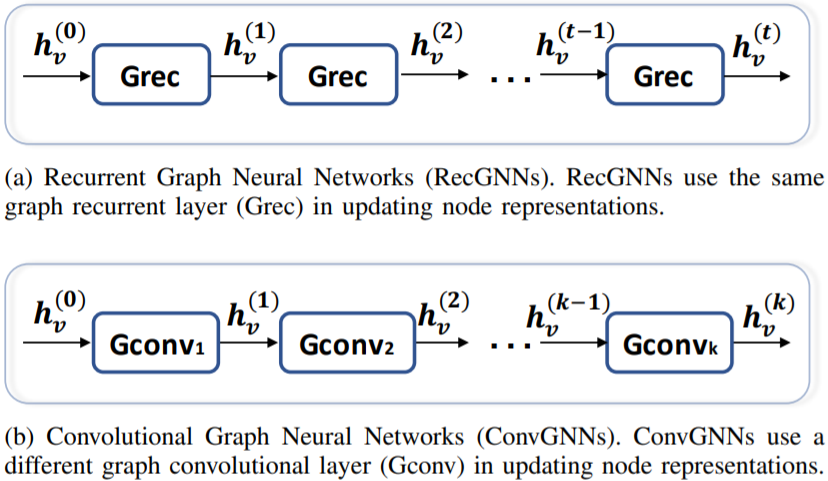
\includegraphics[width=.8\textwidth]{pics/recgnns_convgnns.png}
	\caption{RecGNNs v.s. ConvGNNs}
	\label{fig:recgnns_convgnns}
\end{figure}

在这四种GNNs中,ConvGNNs算是发展得最迅猛、相关工作最多的一类了。ConvGNNs又可以分为两类:Spectral-based ConvGNNs和Spatial-based ConvGNNs。

\textbf{Spectral-based}的方法从图信号处理的角度定义了图卷积。Spectral-based默认graph是无向的,spectral下的图卷积需要对图的Laplacian矩阵进行谱分解$\mathbf{L}=\mathbf{U} \Lambda \mathbf{U}^{T}$,对graph signal进行卷积需要进行\textit{graph Fourier transform},即$\mathscr{F}(\mathbf{x})=\mathbf{U}^{T} \mathbf{x}$,其中$\boldsymbol{x}$为输入的graph signal。图傅里叶变换能够将graph signal变换到由$\boldsymbol{U}$定义的正交空间中。那么给定一个filter(和图像处理领域的滤波器很像)$\boldsymbol{g}$,那么对一个graph signal的卷积定义如下:
$$
\begin{aligned}
	\mathbf{x} *_{G} \mathbf{g} &=\mathscr{F}^{-1}(\mathscr{F}(\mathbf{x}) \odot \mathscr{F}(\mathbf{g})) \\
	&=\mathbf{U}\left(\mathbf{U}^{T} \mathbf{x} \odot \mathbf{U}^{T} \mathbf{g}\right)
\end{aligned}
$$
那么Spectral CNN的定义如下,其中$\Theta_{i, j}^{(k)}$是需要学习的滤波器:
$$
\mathbf{H}_{:, j}^{(k)}=\sigma\left(\sum_{i=1}^{f_{k-1}} \mathbf{U} \Theta_{i, j}^{(k)} \mathbf{U}^{T} \mathbf{H}_{:, i}^{(k-1)}\right) \quad\left(j=1,2, \cdots, f_{k}\right)
$$
spectral-based的图卷积有很坚实的数学基础,但也存在一些局限性:
\begin{itemize}
	\item 不同的结点排列会产生不同的谱分解 --- 不是结点排列无关的
	\item 学习到的滤波器是领域相关的 --- 难以应用到其他领域
	\item 矩阵分解计算复杂 --- 难以应用到large scale graph上
\end{itemize}

\textbf{Spatial-based}即空域的图卷积,是目前的主流。空域的图卷积与图像中的CNN很像。过程:将邻居结点的信息汇聚后,再通过某个函数将结点自身的信息与汇聚后的邻居信息结合起来,与spectral-based的方法相比更直观。在空域卷积的基础上还诞生了图注意力网络 Graph Attention Network。与基础的空域卷积相比,结点与其邻居结点间的权重改由注意力替代。二者的比较如Fig.\ref{fig:gcn_gat}所示:
\begin{figure}[h]
	\centering
	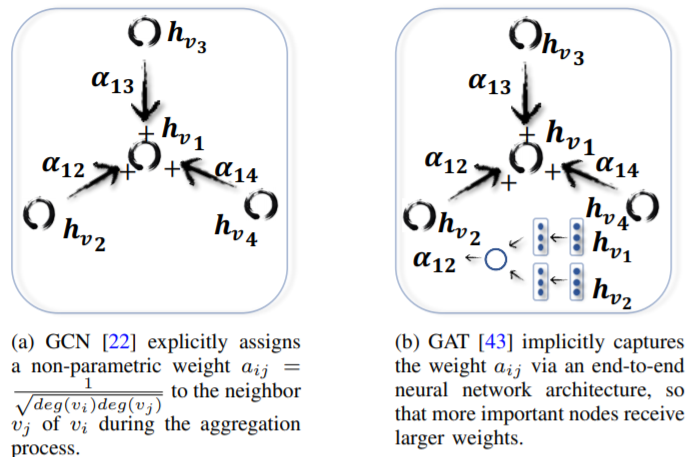
\includegraphics[width=.8\textwidth]{pics/gcn_gat.png}
	\caption{Difference between GCN and GAT}
	\label{fig:gcn_gat}
\end{figure}

除了GAT还出现了与图像领域中类似的操作,如Graph Pooling,功能也与图像领域的池化操作类似 --- 降低图的规模/从结点表征矩阵产生图表征(Readout)。

\subparagraph{GAEs}
图自编码器 --- encoder将graph的结点映射到隐空间中,decoder将隐空间中的图还原/重建。GAEs可以用来学习结点的表征以及生成图。一个现有的GAEs的一个统计表如Fig.\ref{fig:gaes}所示。
\begin{figure}[h]
	\centering
	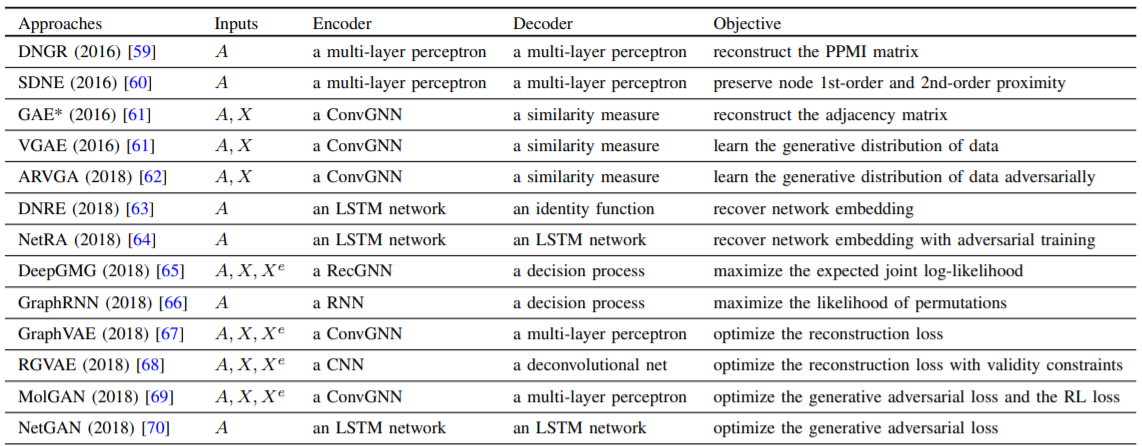
\includegraphics[width=.8\textwidth]{pics/gaes.png}
	\caption{ Main characteristics of selected GAEs}
	\label{fig:gaes}
\end{figure}
使用GAEs来生成图可以分为两类:Sequential --- 逐步地增减结点/边,Global --- 一次性生成整个graph。

\subparagraph{STGNNs}
时空地图神经网络,这种GNNs主要用在dynamic graphs上 --- 捕捉时间序列地特征/分布,序列与graph的联合/边缘分布,graph在时间、空间上的关系。STGNNs的任务可以是预测预测结点的值/标签或者graph的便签 --- 当然是结合时间的。常见的应用场景包括流式的图数据、交通数据(如交通中的流量、速度等数据)等。STGNNs目前主要由两个发展方向:RNN-based和CNN-based。

RNN-based方法会单独处理每一个时刻的图数据,并作为输入流入下一个时刻的处理步骤。有些方法会将结点和边分开来处理 --- 分别输入RNN-based处理单元中。CNN-based方法以非循环的方式来处理,RNN-based和CNN-based有点像RecGNNs和ConvGNNs,CNN-based方法通过堆叠多层网络来处理dynamic graph。

\paragraph{GNNs应用}
\subparagraph{Computer Vision}
包括场景图生成、点云数据分类、动作识别。在场景图中,GNNs可以帮助识别对象之间的语义关系,与之相反的是场景图的生成,将自然语言描述的场景生成为场景图。

\subparagraph{Natural Language Processing}
GNNs可以借助文本中句子/词之间的关系来对文本进行分类,除此之外,在NLP领域还有很多自然的grpah-like数据,如语法依存树。同时也可以基于语义图(semantic graph)来生成文本或者反过来。

\subparagraph{Traffic}
例如动态预测道路的可行驶速度、流量等,这通常与STGNNs联系起来。通常将交通网络看作时空图,其中的结点为安装在路上的传感器、边表示传感器之间的距离,这样每个结点在一定的时间区间内都有自己的流速。

\subparagraph{Recommender system}
Graph-based的推荐系统通常将用户、商品视作结点,通过利用结点之间的关系以及与相关的信息融合起来进行推荐。推荐系统的一个关键点:针对一个用户,给出每个商品对其的重要性排序/分数,这也可以转化为一个链接预测问题 --- 预测用户和商品之间的链接。

\subparagraph{Chemistry}
在生物/化学/生物信息领域,通常利用GNNs来研究分子/化合物/药物的结构 --- 这些东西也天然地具有graph结构。

\subparagraph{Others}
除了上述的几个主要的应用领域,还存在一些比较小众/还未广泛研究的领域,例如程序验证、程序推理、社会影响力预测、对抗攻击防御、异常检测、脑网络研究等。

\paragraph{GNNs模型评估}
在GNNs中有几个主要的任务:结点分类、图分类、链接预测(我自己补充的)。

\paragraph{常用数据集}
常见的数据如Fig.\ref{fig:benchmark}所示.
\begin{figure}[h]
	\centering
	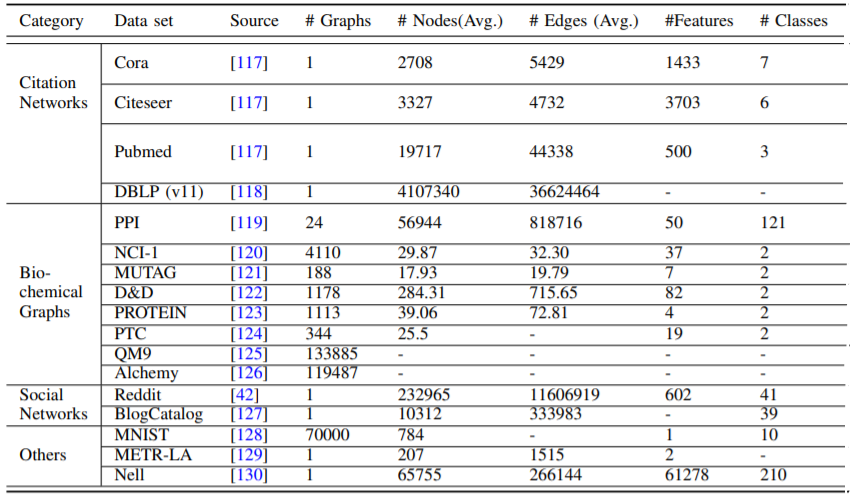
\includegraphics[width=.8\textwidth]{pics/benchmark_datasets.png}
	\caption{Summary of benchmark datasets}
	\label{fig:benchmark}
\end{figure}

\paragraph{未来发展方向}
\subparagraph{Model Depth}
就目前的情况来看,GNNs的模型都比较浅,与CNN模型动则数十层的模型相比,GNNs的模型层数都比较少。当GNN中层数较多时,基本上每个结点的信息都已经被传播到了图中其余的结点 --- 通常图的最短路径会在6跳左右/六度分隔,这也导致当层数一多,图中结点的表征就会趋于一致,这反而使得结点的表征不具有区分性。\tbc{red}{如何加深GNNs或者什么情况下需要深度的GNNs是一个很值得研究的问题}。

\subparagraph{Scalability trade-off}
伸缩性权衡。GNNs的可伸缩性是以破坏图的完整性为代价的。在现有的GNNs中,通常会有ZPooling和Coarsening操作来降低节点特征的维度或者图的规模,但是这些操作都或多或少的丢失了一部分信息。如何设计一个破坏图数据完整性的GNN或者如何权衡完整性和可行性是一个很值得研究的问题。

\subparagraph{Hetergenity}
GNNs在异质图数据上的应用。目前大多数的GNNs处理的是同质的图数据 --- 结点都为同一类型或者只有一种类型,边也只有一种类型,但是还有很多数据是异质的 --- 结点/边的类型是多样的,以及结点/边的输入形式都是不一样的,例如结点/边为文本/图像等,这可以视作现在的多模态融合问题,相当于以GNNs来进行多模态数据融合。

\subparagraph{Dynamicity}
虽然已经有STGNNs来处理随时间变化的图数据,但是大部分都没有dynamic spatioal relations(\textbf{这里我不太理解})。不过确实需要设计更好的处理动态的图数据、流式的图数据(\tbc{red}{流式的数据处理是一个很有意思的问题})。

这篇综述是2019年发表的,虽然在2020年已经出现了很多新的关于GNNs的工作,一些工作也与文中谈的一些问题重叠了,但是这篇综述依然是一片很全面、详细的对GNNs今年来的工作的总结,提出的问题也很具有参考性,是一篇非常棒的综述!






\subsection{The Emerging Field of Signal Processing on Graphs}
\begin{center}

  \begin{tabular}{rp{16cm}lp{20cm}}%{rl}

  % after \\: \hline or \cline{col1-col2} \cline{col3-col4} ...

  论文地址:& \href{https://ieeexplore.ieee.org/stamp/stamp.jsp?tp=&arnumber=6494675}{https://ieeexplore.ieee.org/stamp/stamp.jsp?tp=\&arnumber=6494675} \\
  来源:& IEEE Signal Processing Magazine, 2013 \\
  作者:& David I Shuman, Sunil K. Narang, Pascal Frossard et.al \\

  %源码:& \href{xxx}{xxx} \\

%  slides:& \href{http://yunshengb.com/wp-content/uploads/2017/03/nips_2018_r2l_workshop_talk.pdf}{{\footnotesize Convolutional Set Matching for Graph Similarity}}\\

  关键词:& \textbf{graph signal, signal processing, network analysis} \\

  写于:& \date{2021-01-15}

  \end{tabular}

\end{center}

该论文\cite{6494675}写于2013年,对当时兴起的图信号处理领域进行了总结,主要的内容包括:领域内的主要挑战、定义图谱(graph spectral)领域的不同方法、处理图信号时应用图的不规则结构的重要性、将一些信号处理领域的操作推广到图信号处理领域。

怎么写这篇论文的笔记呢?其实这篇论文我也看的不是很懂,里面涉及很多信号处理领域的理论,也需要较强的数学功底,特别是很多操作是在傅里叶变换的基础上定义的,具体的理论部分我只是浅尝辄止。

论文中首先介绍graph形式的数据在生活中的广泛,当然现在已经有更多的graph形式的数据被发现。既然是图上的信号处理,那能不能将现有的信号处理的方法应用到图信号上呢?当然是可以的,但是也不能生搬硬套,\tbc{red}{如何将现有的信号处理理论方法迁移到图信号上}就是一个挑战。

紧接着论文介绍了谱图领域。图信号可以用$\mathbb{R}^N$中的一个点来表示(n为图中结点数),并用图Laplacian矩阵定义了图信号的傅里叶变换。图信号可以在顶点域(vertex domain)和谱域(spectral domain)中定义,先前的定义是在顶点域上的定义。

最重要的部分就是将传统信号处理领域的理论和方法推广到图信号上了。推广的对信号的操作包括滤波(频率域和顶点域)、卷积、平移、调制和膨胀、图的粗化和下采样、readout等。


一些领域内开放的问题:
\begin{itemize}
	\item 如何使用Laplacian
	\item 图中结点距离的度量方式很多,该使用哪种
	\item 对于大图,很多矩阵分解的方法不再适用
	\item 如何将图信号的性质与图的性质联系起来
\end{itemize}

\subsection{Representation Learning: A Review and New Perspectives}
\begin{center}

  \begin{tabular}{rp{16cm}lp{20cm}}%{rl}

  % after \\: \hline or \cline{col1-col2} \cline{col3-col4} ...

  论文地址:& \href{https://ieeexplore.ieee.org/stamp/stamp.jsp?tp=&arnumber=6472238}{https://ieeexplore.ieee.org/stamp/stamp.jsp?tp=\&arnumber=6472238} \\
  来源:& IEEE TRANSACTIONS ON PATTERN ANALYSIS AND MACHINE INTELLIGENCE, 2013 \\
  作者:& Yoshua Bengio, Aaron Courville, and Pascal Vincent \\

 % 源码:& \href{xxx}{xxx} \\

%  slides:& \href{http://yunshengb.com/wp-content/uploads/2017/03/nips_2018_r2l_workshop_talk.pdf}{{\footnotesize Convolutional Set Matching for Graph Similarity}}\\

  关键词:& \textbf{deep learning, representation learning, feature learning} \\

  写于:& \date{2021-01-26}

  \end{tabular}

\end{center}

该论文\cite{6472238}写于2013年,虽然有一点久远了,但全文内容十分充实、全面,不愧是Bengio巨佬的论文。该文主要对无监督的表征学习进行了总结,内容涵盖了概率模型、自编码器、流形学习以及神经网络。

机器学习的效果严重依赖于输入的数据 --- 即特征工程,在机器学习相关的任务中大部分的时间其实都花在了处理数据、构建特征上。特征工程通常作为下游任务的输入,对于构建的特征,有一个很通用的标准:要有区分性。

\paragraph{表征学习的应用}
\subparagraph{语音识别与信号处理}
\subparagraph{目标识别}
\subparagraph{自然语言处理}
\subparagraph{多任务学习、迁移学习、领域适应}

\paragraph{表征学习中的Priors}
\subparagraph{Smothness}
输入空间中相近的数据点在表征空间中也应该是相近的。相近的概念要看各个空间中距离是如何定义的。这是最基本的一个prior,但可能会导致curse of dimensionality。通常输入空间中样本的分布是很复杂的,在表征空间中会对输入空间进行一定的压缩,这会导致在表征空间中产生一些wrinkles --- 可能有一些导数很大或者不可导的区域。为了在表征空间中尽量连续,则需要大量的数据来“抹平”这些wrinkles。当输入空间的维数增大时,为了“抹平”wrinkles所需的数据将呈指数形式增长 --- curse of dimensionality。

\subparagraph{Multiple explanatory factors}
输入的数据可能是由一些潜在的因素生成的 --- “有一双魔掌在控制着世间万物的生灭”。

\subparagraph{A hierarchical organization of explanatory factors}
潜在因素可以通过层次化的结构进行组织,即我们对数据的抽象是层次化的、逐步的。

\subparagraph{Semi-supervised learning}
当我们使用数据去预测目标时,控制输入数据的潜在因素同样也能控制目标。对$P(X)$有用的表征同样对$P(Y|X)$也是有用的。其实,我感觉这也可以从层次化的角度来看,目标可以看作输入的更深层次的抽象,输入和目标都是受潜在因素控制的,只不过二者的抽象程度不同。

\subparagraph{Shared factors across tasks}
不同的任务之间是会共享一些潜在因素的,这也是迁移学习有效果的原因之一。

\subparagraph{Manifold}
数据空间中,样本点并不是随机或者均匀分布的,而是呈现聚集的状态,数据会集中地占据空间的一部分。不同类型的数据之间数据点密度是较低的。

\subparagraph{Natural clustering}
同类的数据在输入/表征空间中应该是自然聚集的。

\subparagraph{Temporal and spatial coherence}
输入空间中的微小变化也对应着目标空间中的微小变化,与函数的连续性很相似。

\subparagraph{Sparsity}
给定一个样本点$x$,只有一部分因素与之相关,具体来看,表征向量大部分维上取值维0,既可以表示为表征向量对输入的微小变化是不敏感的。

\subparagraph{Simplicity of factor dependencies}
良好的表征,因素之间的关系应该是尽量简单的,如相互独立、线性关系等。

\paragraph{What makes a Representation Good?}
首先,当然应该包含上述的Priors。其次,还有以下因素:
\subparagraph{Distributed representation}
\subparagraph{Depth and Abstraction}
通常表征学习模型具有一定的深度 --- 在学习数据表征的过程中是有一定层次的,能够帮助产生逐步抽象的数据。抽象的数据表征对一些变化是具有不变性的,如平移、旋转、缩放等。

\subparagraph{Disentangling Factors of Variation}
潜在因素之间尽可能使独立的。

\subparagraph{Good Criteria for  Learning Representation?}

接下来论文对如何构建deep representation进行了介绍,比如通过逐层训练的方式来学习深度模型。

在表征学习中,主要可以分为两个流派:概率图模型、神经网络模型。可以简单的区分二者:隐藏单元是被视为隐变量还是可计算结点。接下来就是介绍各种模型了,其中概率模型一直没看懂,都是通过输入、表征的概率分布来建模的,一般是通过最大化似然概率来求解。

接下来是直接学习一个映射将数据从输入空间映射到表征空间,主要介绍了自编码器、regularized autoencoders。在去噪自编码器(从含噪声的样本中能够重建出无噪的样本)中,这需要借助一个假设:样本点使流形数据,数据点是聚集的。加入噪声后的数据会从一定程度上偏离流形,偏离到密度更低的区域。

其实,表征学习可以看作流形学习。有这么一个假设:真实世界中的数据所处的空间是非常大的,甚至是无限维的,数据可以用一个更低维的空间来表示。接下来论文就介绍了一些流形学习的方法。

接下来论文介绍了训练深度模型时的一些问题,如1)参数初始化的重要性;2)参数稀疏性的重要性,当大部分参数一起更新时,目标函数可能会在多个方向上移动,这使得收敛变得困难;3)数值计算的问题,如病态方程等;4)标记数据对模型的效果的提升。

这篇论文真的是非常厚重了,内容足足的,可惜还有不少内容我看不太懂,哎,巨佬就是巨佬啊,非一日之功啊!
}{}

\ifthenelse{\boolean{dlml}}{
\clearpage
\section{DL / ML theory}
\subsection{Auto-Encoding Variational Bayes}
\begin{center}

  \begin{tabular}{rp{16cm}lp{20cm}}%{rl}

  % after \\: \hline or \cline{col1-col2} \cline{col3-col4} ...

  论文地址:& \href{https://arxiv.org/abs/1312.6114}{https://arxiv.org/abs/1312.6114} \\
  来源:& CoRR, 2013 \\
  作者:& Diederik P Kingma, Max Welling \\
  %源码:& \href{xxx}{xxx} \\

%  slides:& \href{http://yunshengb.com/wp-content/uploads/2017/03/nips_2018_r2l_workshop_talk.pdf}{{\footnotesize Convolutional Set Matching for Graph Similarity}}\\

  关键词:& \textbf{Variational Bayes, Auto-Encoding, Bayes Inference, Probalistic Model} \\

  写于:& \date{220-11-09}

  \end{tabular}

\end{center}

论文\cite{kingma2014autoencoding}为bayes概率图模型难以求解的问题提供了一种有效的思路,利用auto-encoding方法结合variational lower bound求解bayes图模型隐变量的后验分布。

在推断和学习中,我们可以认为数据是根据某个隐变量生成的 --- 可以从数据得到隐变量,也能够根据隐变量得到数据 --- 就像一个编码、解码的过程。但是,通常隐变量的分布是未知的、复杂的,难以通过假定一个已知的分布来近似隐变量的真实分布。

简单谈一下个人对隐变量的理解:宽泛的讲,隐变量就像现实背后的某种神秘的、未知的因素,我们所见的现实背后蕴含着这种神秘的因素 --- 隐变量,但我们通常是看不到隐变量的,也无法对它进行直接的观测,比如直接描述它是什么、它的形式、它发生的概率等等。但当我们得知隐变量后我们就像获得了某种神奇的力量,知道隐变量发生后现实中会发生什么。从数据的角度来看,隐变量可以是数据背后的“真理” --- 特征、数据产生的原因。当我们能够描述隐变量后,我们就能够根据隐变量生成我们想要的数据。这就像一个编码-解码的过程,将原始数据编码为特征,再根据特征产生数据。

\begin{figure}[h]
	\centering
	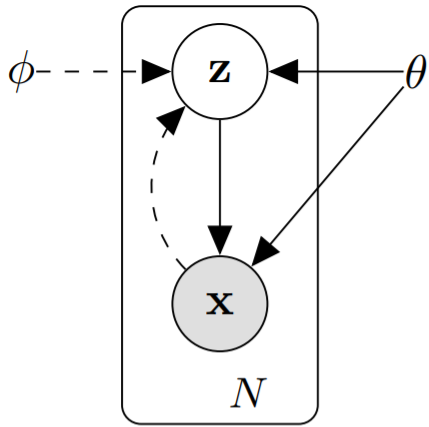
\includegraphics[width=.18\textwidth]{pics/AEVB.PNG}
	\caption{有向图模型}
	\label{fig:aevb}
\end{figure}

那么问题来了:\tbc{red}{如何得到隐变量呢?}

如图\ref{fig:aevb}所示,图中实线可以看作生成(即解码)过程 --- $p_{\theta}(\boldsymbol{z})p_{\theta}(\boldsymbol{x}|\boldsymbol{z})$,虚线可以看作编码过程 --- $q_{\phi}(\boldsymbol{z}|\boldsymbol{x})$。$\theta$表示真实的分布的参数,$\phi$表示近似ho后验分布的参数 --- 该近似分布用于近似真实的后验分布$p_{\theta}(\boldsymbol{z}|\boldsymbol{x})$。为了使近似分布$q_{\phi}(\boldsymbol{z}|\boldsymbol{x})$和真实分布$p_{\theta}(\boldsymbol{z}|\boldsymbol{x})$尽量相同,可以使用KL散度进行衡量。

\begin{equatiopn}%\nonumber
	\begin{align}
		KL(q_{\phi}(\boldsymbol{z}|\boldsymbol{x})||p_{\theta}(\boldsymbol{z}|\boldsymbol{x})) &= E_{q_{\phi}(\boldsymbol{z}|\boldsymbol{x})}[ \log \frac{q_{\phi}(\boldsymbol{z}|\boldsymbol{x})}{p_{\theta}(\boldsymbol{z}|\boldsymbol{x})} ] \notag \\
		&= E_{q_{\phi}(\boldsymbol{z}|\boldsymbol{x})}[ \log q_{\phi}(\boldsymbol{z}|\boldsymbol{x}) - \log {p_{\theta}(\boldsymbol{z}|\boldsymbol{x})} ] \notag \\
		&= E_{q_{\phi}(\boldsymbol{z}|\boldsymbol{x})}[ \log q_{\phi}(\boldsymbol{z}|\boldsymbol{x}) - \log \frac{p_{\theta}(\boldsymbol{z},\boldsymbol{x})} {p_{\theta}(\boldsymbol{x})} ] \notag \\
		&= E_{q_{\phi}(\boldsymbol{z}|\boldsymbol{x})}[ \log q_{\phi}(\boldsymbol{z}|\boldsymbol{x}) - \log p_{\theta}(\boldsymbol{z},\boldsymbol{x}) + \log p_{\theta}(\boldsymbol{x}) ] \notag \\
		&= E_{q_{\phi}(\boldsymbol{z}|\boldsymbol{x})}[ \log q_{\phi}(\boldsymbol{z}|\boldsymbol{x}) - \log p_{\theta}(\boldsymbol{z},\boldsymbol{x})] + \log p_{\theta}(\boldsymbol{x})   \label{eq:kl}
	\end{align}
\end{equatiopn}
由公式(\ref{eq:kl})可得,对于训练数据中的每一个样本有:
$$
\log p_{\theta}(\boldsymbol{x}^{(i)}) = KL(q_{\phi}(\boldsymbol{z}|\boldsymbol{x}^{(i)})||p_{\theta}(\boldsymbol{z}|\boldsymbol{x}^{(i)})) + \mathcal{L}(\theta, \phi; \boldsymbol{x}^{(i)})
$$
其中,
$$\mathcal{L}(\theta, \phi; \boldsymbol{x}^{(i)}) = E_{q_{\phi}(\boldsymbol{z}|\boldsymbol{x})}[ -\log q_{\phi}(\boldsymbol{z}|\boldsymbol{x}) + \log p_{\theta}(\boldsymbol{z},\boldsymbol{x})]
$$
因为KL是大于等于零的,那么显然有这样的关系:$\log p_{\theta}(\boldsymbol{x}^{(i)}) \ge \mathcal{L}(\theta, \phi; \boldsymbol{x}^{(i)})$。所以$\mathcal{L}(\theta, \phi; \boldsymbol{x}^{(i)})$又叫做变分下界(variational lower bound)。$\log p_{\theta}(\boldsymbol{x}^{(i)})$相当于样本的对数似然函数,当给定了数据后,其实$\log p_{\theta}(\boldsymbol{x}^{(i)})$应该是确定的,那么为了使近似分布尽量接近真实分布,那么则应该让变分下界尽可能的大,这样近似分布就会尽可能地接近真实分布。OKAY!现在问题转化成了最大化$\mathcal{L}(\theta, \phi; \boldsymbol{x}^{(i)})$了。

那么问题又来了:\tbc{red}{如何最大化变分下界呢?}

经过一顿操作后,变分下界可写为:
$$\mathcal{L}(\theta, \phi; \boldsymbol{x}^{(i)}) = -KL(q_{\phi}(\boldsymbol{z}|\boldsymbol{x}^{(i)})||p_{\theta}(\boldsymbol{z})) + E_{q_{\phi}(\boldsymbol{z}|\boldsymbol{x}^{(i)})}[\log p_{\theta}(\boldsymbol{x}^{(i)}|\boldsymbol{z})]
$$
其中第一项可以看作正则化项(当增加隐变量的数量时,可以防止过拟合),第二项可以看作重构损失。为了最大化变分下界,可以使用梯度下降的方法,但是上式中变分下界难以计算,且近似分布$q_{\phi}(\boldsymbol{z}|\boldsymbol{x}^{(i)})$是未知的。如果直接使用蒙特卡洛方法计算变分下界,将会带来较大方差。论文中针对这个问题使用了重参数化(reparameterization)来表示隐变量:$\hat{\boldsymbol{z}} = g_{\phi}(\boldsymbol{\epsilon}, \boldsymbol{x})$,其中$\boldsymbol{\epsilon}$服从于某个分布$p(\boldsymbol{\epsilon})$。那么问题就转化成了选择合适的函数$g$和分布$p(\boldsymbol{\epsilon})$。已知一个函数关于其自变量的后验分布的的蒙特卡洛估计为下式:
$$
E_{q_{\phi}(\boldsymbol{z}|\boldsymbol{x}^{(i)})}[f(\boldsymbol{z})] = E_{p(\boldsymbol{\epsilon})}[f(g_{\phi}(\boldsymbol{\epsilon}, \boldsymbol{x}^{(i)} ) ) ] \simeq \frac{1}{L} \sum_{l=1}^{L} f(g_{\phi}(\boldsymbol{\epsilon}^{(l)}, \boldsymbol{x}^{(i)} ) )
$$
其中$L$为对每个数据$\boldsymbol{x}^{(i)}$进行蒙特卡洛采样的次数。那么使用蒙特卡洛估计重参数化后的变分下界,形式为:
$$
\mathcal{L}(\theta, \phi; \boldsymbol{x}^{(i)}) =  \frac{1}{L} \sum_{l=1}^{L} \log p_{\theta}(\boldsymbol{z}^{(i, l)},\boldsymbol{x}^{(i)}) - \log q_{\phi}(\boldsymbol{z}^{(i, l)}|\boldsymbol{x}^{(i)})
$$
其中,$\boldsymbol{z}^{(i, l)}=g_{\phi}(\boldsymbol{\epsilon}{(i, l)}, \boldsymbol{x}{(i)}), \boldsymbol{\epsilon}^{(l)} \sim p(\boldsymbol{\epsilon})$。之后便可以使用小批量的随机梯度下降算法优化参数$\theta, \phi$。

关于VAE的tutorial可以参考:\href{https://arxiv.org/pdf/1606.05908.pdf}{Tutorial on Variational Autoencoders}。未使用重参数化技巧与使用了重参数化技巧对比如Fig.\ref{fig:vae_rp}\cite{doersch2016tutorial}所示:
\begin{figure}[h]
	\centering
	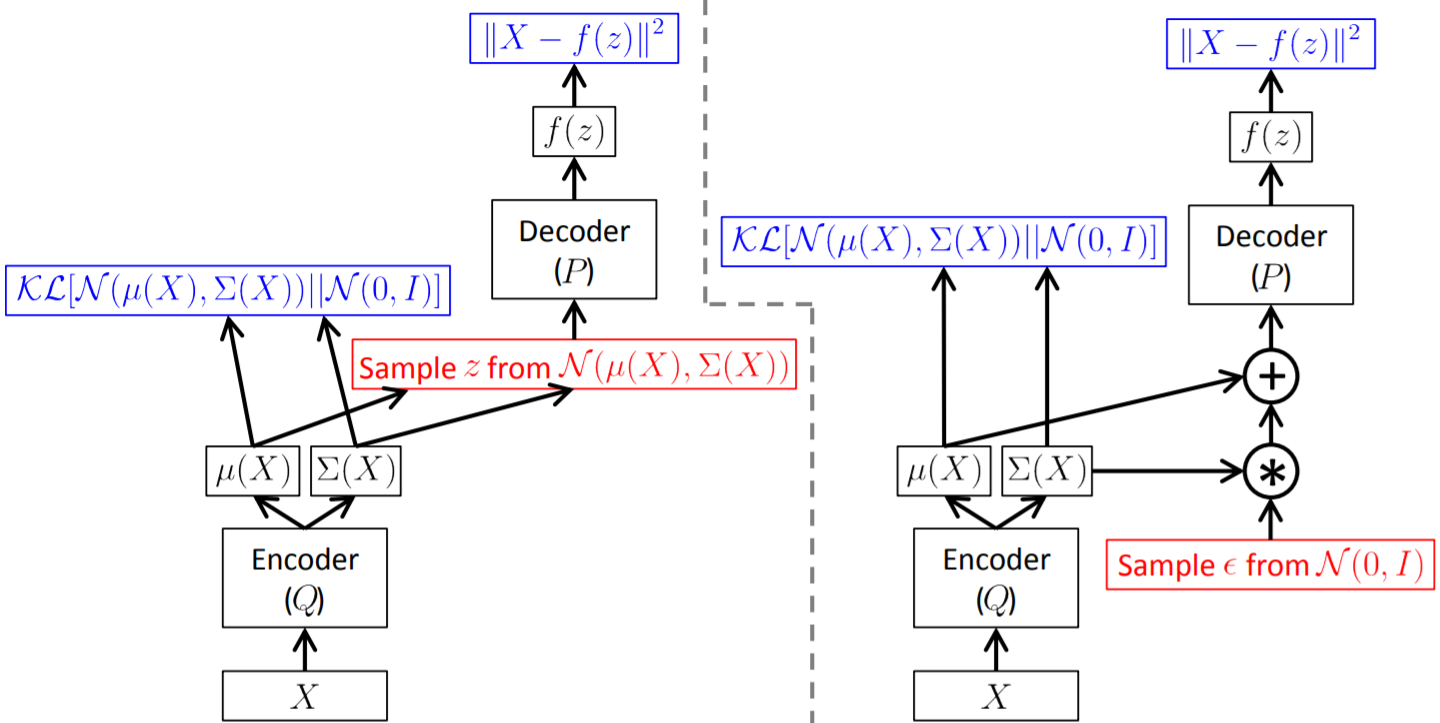
\includegraphics[width=.8\textwidth]{pics/vae_rp.png}
	\caption{without vs. with reparameterization}
	\label{fig:vae_rp}
\end{figure}

一些网上的参考资料:
\begin{itemize}
	\item \href{https://www.cnblogs.com/yifdu25/p/8181185.html}{变分推断}
\end{itemize}

\paragraph{方法解决的问题/优势}

\begin{itemize}
	\item 从参数化变分下界,使得能够使用随机梯度下降算法优化参数
	%\item 

\end{itemize}


\paragraph{方法的局限性/未来方向}

\begin{itemize}
	\item 时序模型
	\item 具有隐变量的监督学习模型,可用于学习复杂的噪声分布

\end{itemize}








\subsection{Adversarial Autoencoders}
\begin{center}

  \begin{tabular}{rp{16cm}lp{20cm}}%{rl}

  % after \\: \hline or \cline{col1-col2} \cline{col3-col4} ...

  论文地址:& \href{https://arxiv.org/abs/1511.05644}{https://arxiv.org/abs/1511.05644} \\
  来源:& ICLR, 2016 \\
  作者:& Alireza Makhzani ,Jonathon Shlens ,Navdeep Jaitly ,Ian Goodfellow ,Brendan Frey \\
  源码:& \href{https://github.com/fducau/AAE_pytorch}{AAE\_pytorch} \\

%  slides:& \href{http://yunshengb.com/wp-content/uploads/2017/03/nips_2018_r2l_workshop_talk.pdf}{{\footnotesize Convolutional Set Matching for Graph Similarity}}\\

  关键词:& \textbf{GAN, Autoencoder, Generative Models} \\

  写于:& \date{2020-12-20}

  \end{tabular}

\end{center}

论文\cite{makhzani2016adversarial}对autoencoder进行了改进,结合GAN提出了新的generative model。第一次看了一两页,看的很懵,第二次看的时候十分痛快,一个上午就看完了,整篇论文读下来收获很多。Adversarial Autoencoder(AAE)将GAN与autoencoder相结合,仿照GAN的训练方式来训练自编码器网络。通篇看下来,autoencoder、GAN、AAE都成了分布的匹配(拟合)问题。特别是论文提出的AAE,论文将数据分布$p_d(\boldsymbol{x})$的隐变量$\boldsymbol{x}$的分布与某个已知的分布进行匹配/拟合。论文中不仅给出了基础的AAE的架构,如图Fig.\ref{fig:AAE}所示,还给出了AAE在其他方面的应用,如有/无/半监督的AAE、AAE在聚类和降维上的应用,并给出了相应的网络结构,非常棒!

\begin{figure}[h]
	\centering
	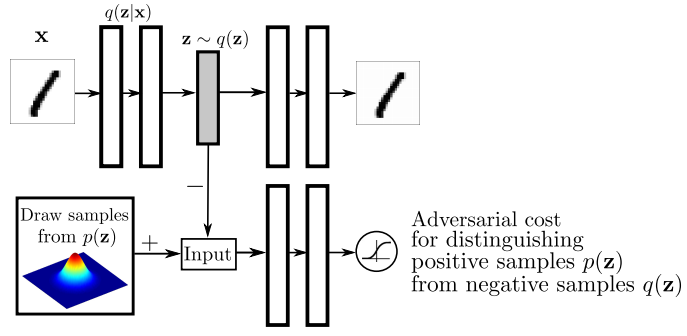
\includegraphics[width=.8\textwidth]{pics/aae.PNG}
	\caption{Architecture of AAE}
	\label{fig:AAE}
\end{figure}

\paragraph{AAE思路}
通常的autoencoder或者VAE\cite{kingma2014autoencoding}在训练时通常是以重建损失或者ELBO为目标,VAE中使用了重参数化的技巧来训练。AAE其实和VAE也是有一点相似之处的:都会从一个确定的分布中进行采样。对AAE而言,整个网络结构分为两部分:autoencoder和discriminator。autoencoder就是普通的自编码器:输入数据学习到数据的隐表示$\boldsymbol{z}$,使用重建损失函数;discriminator与GAN中的D时一致的:从一个已知的先验分布$p(\boldsymbol{z})$中采样一个$\boldsymbol{z}$,这个时候来自autoencoder的$\boldsymbol{z}$作为负样本$\boldsymbol{z}_-$,来自$p(\boldsymbol{z})$作为正样本$\boldsymbol{z}_+$,由D来进行判别,使用判别损失函数。如果与GAN进行比较,可以知道\tbc{red}{$p(\boldsymbol{z})$相当于真是数据分布,而autoencoder中的encoder则相当于GAN中的generator}。上文中还提到了一个很关键的点:\tbc{red}{分布的匹配/拟合}。

这在AAE中体现的尤为明显。上面描述的过程其实也可以抽象为分布的匹配/拟合。已知的分布$p(\boldsymbol{z})$作为一个目标分布,目的是使数据隐变量的分布$p(\boldsymbol{z})$与目的分布一致 --- 判别器无法区分$\boldsymbol{z}$是来自$p(\boldsymbol{z})$还是来自$q(\boldsymbol{z})$。与VAE中的重参数化不同,AAE可以直接使用梯度下降的方法进行训练。AAE的训练过程分为两个阶段:reconstruction和regularization。

在reconstruction阶段:autoencoder通过最小化重建损失来更新encoder和decoder。在regularization阶段:通过对抗损失来更新判别网络和生成网络(也即encoder)。



\paragraph{AAE的应用}
论文中还介绍了AAE的几个主要的应用:
\begin{itemize}
	\item 将标签信息融入到判别器中:以one-hot的形式构造标签编码,将标签编码与从$p(\boldsymbol{z})$中采样到的$\boldsymbol{z}$一起输入到判别网络中
	\item 将标签信息融入到autoencoder中:将one-hot编码的标签信息与数据的隐变量$\boldsymbol{z}$一起输入到decoder中
	\item 半监督的AAE:其实这个相当于将标签信息融入到autoencoder和判别器中。此时的网络结构中将会由两个判别器,分别对$\boldsymbol{z}$和标签信息进行判别,因此也需要为标签信息增加一个generator --- 论文中采用的是categorical分布。此时网络的训练在原基础上增加了一个阶段 --- semi-supervised classification阶段,该阶段使用交叉熵来更新监督损失
	\item 使用AAE进行无监督的聚类:这部分十分有趣!论文中特地针对MINST数据集进行了聚类,但不是聚类成10类,AAE可以将同一个数字的不同风格的图像区分出来 --- 将风格分离了出来
	\item 使用AAE进行降维:此处的AAE与半监督的AAE十分相似。论文中还分析了已有方法进行降维时的几个主要问题:难以应用到新的数据上(T\_SNE解决了这个问题)、数据可能处于流形空间等
\end{itemize}

\paragraph{方法解决的问题/优势}
\begin{itemize}
	\item 将GAN中的discriminator与autoencoder相结合,得到了强大的自编码器
	\item 不需要使用重参数化就能训练,效果比VAE好
	\item AAE的结构修改可以使用到多种任务上,可扩展性极好
\end{itemize}

\paragraph{方法的局限性/未来方向}
\begin{itemize}
	\item 用来学习更好的表征,很棒的特征提取器
	\item \tbc{red}{基于AAE的聚类}
	\item \tbc{red}{基于AAE的降维可视化}
\end{itemize}

\subsection{Attention is All you need}
\begin{center}

  \begin{tabular}{rp{16cm}lp{20cm}}%{rl}

  % after \\: \hline or \cline{col1-col2} \cline{col3-col4} ...

  论文地址:& \href{https://papers.nips.cc/paper/2017/file/3f5ee243547dee91fbd053c1c4a845aa-Paper.pdf}{https://papers.nips.cc/paper/2017/file/3f5ee243547dee91fbd053c1c4a845aa-Paper.pdf} \\
  来源:& NIPS, 2017 \\
  作者:& Ashish Vaswani, et al. \\

  源码:& \href{https://github.com/tensorflow/tensor2tensor}{tensor2tensor} \\

%  slides:& \href{http://yunshengb.com/wp-content/uploads/2017/03/nips_2018_r2l_workshop_talk.pdf}{{\footnotesize Convolutional Set Matching for Graph Similarity}}\\

  关键词:& \textbf{Sequecnce Modeling, Neural Machine Translation} \\

  写于:& \date{2021-03-07}

  \end{tabular}

\end{center}

该论文\cite{vaswani2017attention}针对序列转换(Sequence Transduction)问题中常见的弊端,提出使用Attention来完成Sequence Transduction,提出了新的网络结构 --- Transformer。

\paragraph{问题定义}在Sequence Transduction领域中,通常是基于encoder-decoder形式的循环神经网络或CNN的。也存在一些模型使用注意力机制将encoder和decoder连接起来。该论文提出了一种完全基于注意力机制的新型网络 --- Transformer,不需要RNN或CNN。

在对序列进行处理时,RNN通常沿着输入/输出序列的顺序进行计算,将序列中元素的位置与计算的步骤相对齐。这样的处理方式看似天然地保留了序列形式,但是使得计算只能串行进行,难以并行,而且对于长序列的计算还会带来内存容量限制的问题。虽然目前已经有一些相关的工作关于RNN的并行化,但是RNN串行计算的问题依然存在。

注意力机制已经成为了序列建模中不可或缺的一部分,在建模序列中依赖的时候能够不用考虑输入/输出中的距离。但是之前的工作都是用于起连接作用,本文则将encoder-decoder完全建立在注意力机制上来完成序列的建模问题。并在机器翻译任务中检测了Transformer的效果。


\paragraph{Transformer}
\begin{figure}[h]
	\centering
	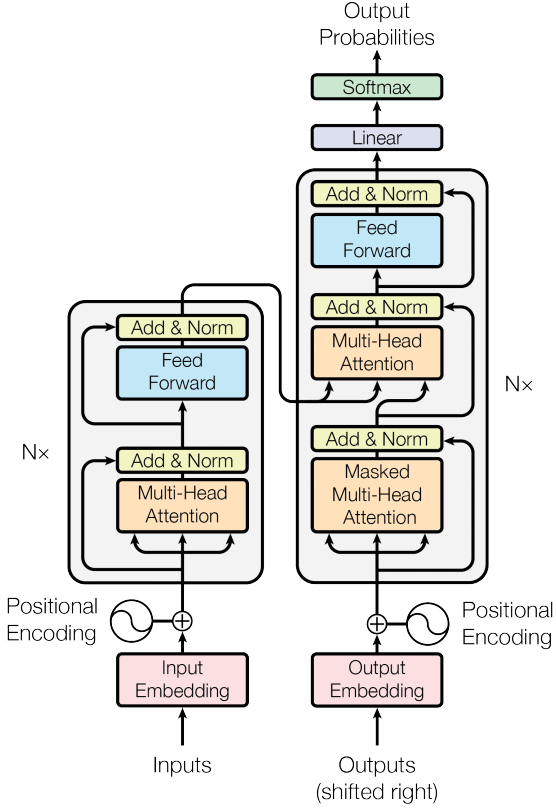
\includegraphics[width=.5\textwidth]{pics/Transformer.PNG}
	\caption{Transformer Architecture}
	\label{fig:transformer}
\end{figure}

\subparagraph{Encoder and Decoder}
Transformer的结构如Fig.\ref{fig:transformer}所示,其中左边为$N$个相同的layer堆叠起来的组成的encoder,右边为$N$个相同的layer堆叠起来组成的decoder。组成encoder的layer又两部分组成:Multi-head Attention、Fully connected Feed Forward。组成encoder的layer由三部分组成:两个Multi-head Attention、Fully connected Feed Forward。以上的Multi-head Attention和Fully connected FFN都有残差连接和layer normalization。这样每一部分的输出都可以表示为:$LayerNorm(x + Sublayer(x))$,其中$Sublayer$就是Multi-head Attention或Fully connected FFN。

其实Encoder和Decoder都是由Multi-head Attention和Fully connected FFN组成的,但是二者在Self-Attention上有一些差别。Decoder修改了Self-Attention,是为了保证\tbc{red}{在预测$i$处的输出时,只能依赖$i$之前的输出,同时也是为了保持自回归(auto-regressive)的性质}。

\subparagraph{Attention}
一个注意力函数可以描述为:将一个query与一系列的key-value对(pair)进行映射得到一个输出,其中的query、keys、values和输出均为向量。输出时values的加权求和,values对应的权是通过query与key计算得到的。

\begin{figure}[h]
	\centering
	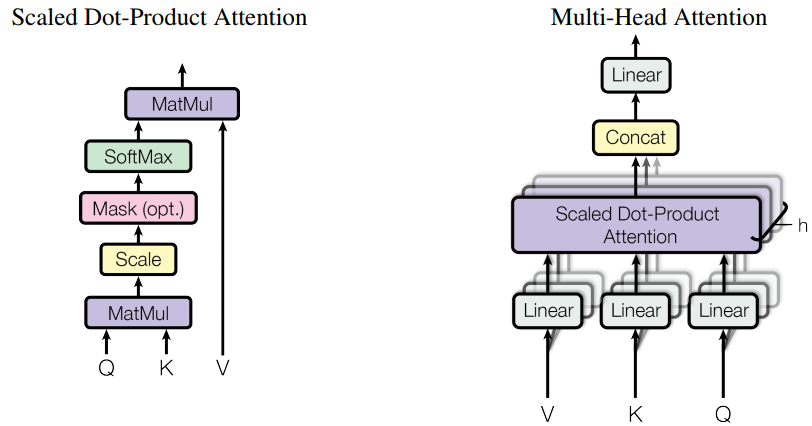
\includegraphics[width=.8\textwidth]{pics/Scaled Dot-Production Attention and Multi-Head Attention.PNG}
	\caption{Scaled Dot-Production Attention与Multi-Head Attention}
	\label{fig:scaled dot-product attention and multi-head attention}
\end{figure}

该论文中采用的是\textbf{Scaled Dot-Product Attention},其计算过程如Fig.\ref{fig:scaled dot-product attention and multi-head attention}所示,写成公式为:
$$
\operatorname{Attention}(Q, K, V)=\operatorname{softmax}\left(\frac{Q K^{T}}{\sqrt{d_{k}}}\right) V
$$
有两种常用的attention函数:additive attention和dot-product attention。该论文中使用的是dot-product attention,但是略微不同,是Scaled后的dot-product attention。\tbc{red}{为什么要对dot-product 进行scaled呢?}
\tbc{green}{当query、key的维度很大时,点积后的值可能会很大,可能会使softmax函数进入梯度很小的区域}。举个例子,假如q和k都是服从均值为0,方差为1的分布的随机变量,那么$q \cdot k = \sum_{i=1}^{d} q_i k_i$,结果的均值为0,但是方差为$d$。

论文中使用了\textbf{Multi-head Attention}。从Fig.\ref{fig:scaled dot-product attention and multi-head attention}可以看出,在进行Multi-head Attention之前,先对Q、K、V进行了线性映射:
$$
\begin{aligned}
	\operatorname{MultiHead}(Q, K, V) &=\text { Concat }\left(\text { head }_{1}, \ldots, \text { head }_{\mathrm{h}}\right) W^{O} \\
	\quad \text { where head }_{\mathrm{i}} &=\text { Attention }\left(Q W_{i}^{Q}, K W_{i}^{K}, V W_{i}^{V}\right)
\end{aligned}
$$

在Multi-Head Attention后就是\textbf{Position-wise Feed-Forward Networks}。从名字 --- Position-wise也可以看出,Multi-head Attention的输出是逐个通过FFN的。\tbc{red}{在输入Attention函数之前,各个位置上的元素可以看作是独立的,不包含元素之间的依赖关系,经过Attention函数后,各个元素不仅包含了本身的含义还包含了与其他元素的依赖关系。所以不需要串行地通过FFN,FFN这一步操作是可以并行化的}。

因为Transformer本身是不包含循环和卷积的,为了使模型利用序列中的顺序,论文中将\textbf{Positional Encoding}“加”到输入序列中的元素上。论文中使用的Positional-Encoding:
$$
\begin{aligned}
	P E_{(p o s, 2 i)} &=\sin \left(p o s / 10000^{2 i / d_{\text {model }}}\right) \\
	P E_{(p o s, 2 i+1)} &=\cos \left(p o s / 10000^{2 i / d_{\text {model }}}\right)
\end{aligned}
$$
其中$pos,d_{model}$分别表示词在序列中的位置和位置向量的维度。作者选用这样的位置编码的原因:\tbc{red}{使不同位置的元素能够通过相对位置更好地与当前元素建立关系,因为对于任意固定的$k$,$PE_{pos+k}$可以表示为$PE_{pos}$的线性函数}。

\paragraph{Why Self-Attention}
$$
\begin{array}{lccc}
	\hline \text { Layer Type } & \text { Complexity per Layer } & \begin{array}{c}
		\text { Sequential } \\
		\text { Operations }
	\end{array} & \text { Maximum Path Length } \\
	\hline \text { Self-Attention } & O\left(n^{2} \cdot d\right) & O(1) & O(1) \\
	\text { Recurrent } & O\left(n \cdot d^{2}\right) & O(n) & O(n) \\
	\text { Convolutional } & O\left(k \cdot n \cdot d^{2}\right) & O(1) & O\left(\log _{k}(n)\right) \\
	\text { Self-Attention (restricted) } & O(r \cdot n \cdot d) & O(1) & O(n / r) \\
	\hline
	\label{rnn-cnn-attention}
\end{array}
$$
与RNN/CNN相比,使用Self-Attention主要有三个原因:
\begin{itemize}
	\item 计算复杂度
	\item 可并行的计算量
	\item 长范围依赖关系中的路径长度(注意:\textbf{长范围的依赖不一定代表距离远})。路径越短,越容易学习到长范围的依赖。Self-Attention中将每个位置的元素都直接与其他位置的元素相连。从Attention的输入和输出来看,CNN和Attention之间是有一定相似性的,如Fig.\ref{fig:cnn-attention-multi head}所示。Multi-head能够捕捉多种关系。在较长的输入序列下,可以选择restricted的self-attention,即每个位置只考虑周围固定数量的邻居
\end{itemize}
三者的比较见Tab.\ref{rnn-cnn-attention}
\begin{figure}[h]
	\centering
	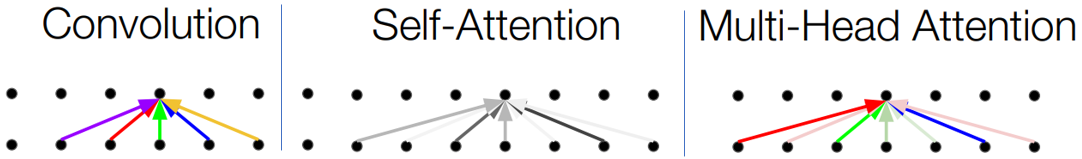
\includegraphics[width=.8\textwidth]{pics/CNN-Attention-Multi head.png}
	\caption{CNN、Attention、Multi-head Attention}
	\label{fig:cnn-attention-multi head}
\end{figure}

\paragraph{方法解决的问题/优势}

\begin{itemize}

	\item 提出了完全基于Attention机制的序列建模
	\item 基于Attention的Transformer中的大量操作都是可以并行的,大大降低计算的时间
	\item 对长范围依赖关系的建模

\end{itemize}



%\paragraph{方法的局限性/未来方向}


\paragraph{Attention参考资料}
\begin{itemize}
	\item \href{http://nlp.seas.harvard.edu/2018/04/03/attention.html}{The Annotated Transformer --- Harvard Transformer tutorial}
	\item \href{https://jalammar.github.io/visualizing-neural-machine-translation-mechanics-of-seq2seq-models-with-attention/}{Visualizing A Neural Machine Translation Model (Mechanics of Seq2seq Models With Attention)}
	\item \href{https://jalammar.github.io/illustrated-transformer/}{The Illustrated Transformer}
\end{itemize}





\subsection{Deep Residual Learning for Image Recognition}
\begin{center}

  \begin{tabular}{rp{16cm}lp{20cm}}%{rl}

  % after \\: \hline or \cline{col1-col2} \cline{col3-col4} ...

  论文地址:& \href{https://ieeexplore.ieee.org/stamp/stamp.jsp?tp=\&arnumber=7780459}{https://ieeexplore.ieee.org/stamp/stamp.jsp?tp=\&arnumber=7780459} \\
  来源:& CVPR, 2016\\
  作者:& Kaiming He Xiangyu Zhang, et al. \\

  源码:& \href{https://github.com/KaimingHe/deep-residual-networks}{deep-residual-networks} \\

%  slides:& \href{http://yunshengb.com/wp-content/uploads/2017/03/nips_2018_r2l_workshop_talk.pdf}{{\footnotesize Convolutional Set Matching for Graph Similarity}}\\

  关键词:& \textbf{Residual Learning, Shortcut Connection} \\

  写于:& \date{2021-03-15}

  \end{tabular}

\end{center}

该论文\cite{he2016deep}主要解决的深层神经网络的训练问题。随着网络的深度的增加,模型的效果反而变差了,论文提出了Residual Learning的方式来训练深层的神经网络。

\paragraph{问题定义}
基于深度神经网络模型在图像领域的很多任务上都取得了重大的突破,其中模型的深度起到了关键性的作用。但是随着模型深度的增加,一系列问题出现了:\textbf{深度的模型只是堆叠更多的层就可以了吗?}随着层数的增加,会出现梯度消失/爆炸问题,这个问题可以通过不同的归一化来解决。但还有一个问题:degradation --- 模型退化。Degradation是论文解决的问题。那么什么是模型退化呢?
\begin{figure}[h]
	\centering
	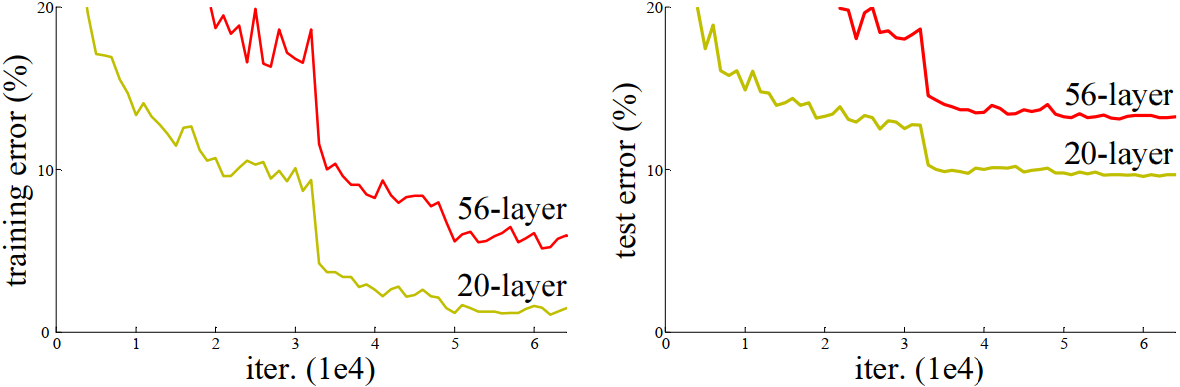
\includegraphics[width=.5\textwidth]{pics/degradation.png}
	\caption{Degradation}
	\label{fig:degradation}
\end{figure}

考虑一个已经训练好的模型,它能达到一定的效果,为了让效果更好,我们在训练好的模型的基础上增加层,再进行训练。按照常理,新增的层就算学习到了恒等映射模型也不会退化的,但是一些实验显示,增加层后的模型的效果不但没有提升反而还下降了!\textbf{模型退化}了!这表明:\tbc{red}{在求解时,使用多个非线性层来近似恒等映射可能是比较困难的}。

\paragraph{Residual Learning}

\begin{figure}[h]
	\centering
	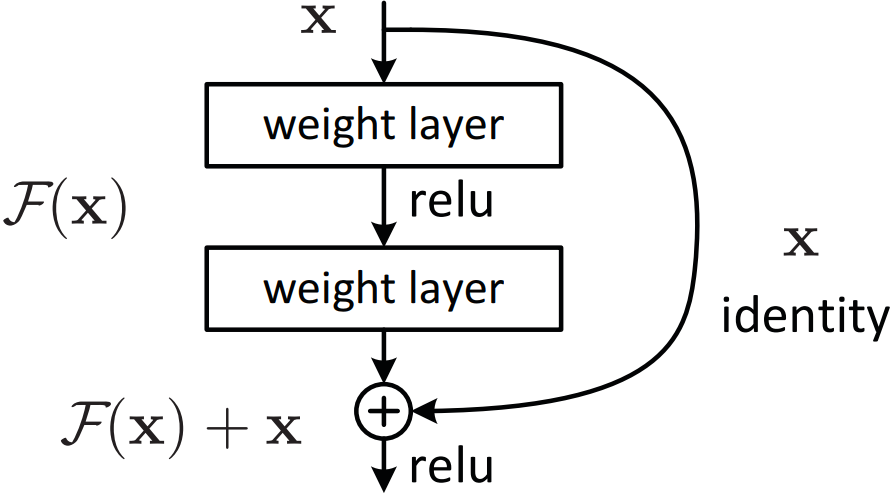
\includegraphics[width=.4\textwidth]{pics/residual.png}
	\caption{Residual learning: a building block}
	\label{fig:residual}
\end{figure}
为了解决模型退化的问题,作者提出了\textit{deep residual learning} framework。
在加深模型时,我们通常希望新加的层能够直接学习到潜在的映射函数$\mathcal{H}(x)$,residual learning并不是如此,而是学习一个residual mapping $\mathcal{F}(x) = \mathcal{H}(x) - x$。那么原来期望学习到的映射就可以表示成:$\mathcal{H}(x) = \mathcal{F}(x) + x$。这里有一个假设:\textbf{$\mathcal{F}$比$\mathcal{H}$更容易优化}。

$\mathcal{F}(x) + x$可以用一个带有shortcut连接的前馈神经网络模拟,如Fig.\ref{fig:residual}所示。如果恒等映射是最优解,那么只需要使residual block中层的参数为零即可。结合之前所说的非线性层难以学习identity,residual block不仅包含了identity部分,还包括了非线性部分,这样的一个映射不仅可以学习到复杂的非线性部分,还可以学习到非线性层难以学习到的线性部分(不仅是identity,还可以是$ax+b$,线性函数加非线性函数)。

Fig.\ref{fig:residual}所示的残差块可以表示为:
$$
\mathbf{y}=\mathcal{F}\left(\mathbf{x},\left\{W_{i}\right\}\right)+  \mathbf{x}
$$
\begin{center}
	或
\end{center}
$$
\mathbf{y}=\mathcal{F}\left(\mathbf{x},\left\{W_{i}\right\}\right)+W_{s} \mathbf{x}
$$
以两层的残差块为例,$\mathcal{F}(x, {W_i}) = W_2\sigma (W_1 x)$表示需要学习的残差函数。当然,除了Fig.\ref{fig:residual}所示的残差块,还可以有三层甚至更多层的残差块。论文中还对shortcut connection的形式进行了实验验证,第二种形式的形式效果可能会稍微好一点点,但是可以忽略,而identity形式的残差具有更少的参数、更低的复杂度。


\paragraph{方法的问题/优势}

\begin{itemize}

	\item 研究深度模型中的退化问题,累积的非线性层可能难以学习到线性映射
	\item 提出了residual learning,助力深度模型的学习,且没有增加学习的参数
	\item 提出了ResNet

\end{itemize}


\paragraph{方法的局限性/未来方向}

\begin{itemize}

	\item 累加的非线性层可能可以学习到较复杂的非线性变化,但是难以通过非线性层学习到线性变换,residual learning弥补了这一缺点
	

\end{itemize}
}{}

\ifthenelse{\boolean{gnntheory}}{
\clearpage
\section{GNN Theory}
\subsection{Variational Graph Auto-Encoders}
\begin{center}

  \begin{tabular}{rp{6cm}lp{12cm}}%{rl}

  % after \\: \hline or \cline{col1-col2} \cline{col3-col4} ...

  论文地址:& \href{https://arxiv.org/abs/1611.07308}{https://arxiv.org/abs/1611.07308} \\

  源码:& \href{https://github.com/tkipf/gae}{gae} \\

%  slides:& \href{http://yunshengb.com/wp-content/uploads/2017/03/nips_2018_r2l_workshop_talk.pdf}{{\footnotesize Convolutional Set Matching for Graph Similarity}}\\

  关键词:& \textbf{Variational auto encoders} \\

  写于:& \date{2020-10-16}

  \end{tabular}

\end{center}

该论文\cite{kipf2016variational}利用VAE(Variational auto-encoder\cite{kingma2014autoencoding})来学习无向图的隐表示,并可以从隐表示解码出原来的图。

\begin{figure}[h]
	\centering
	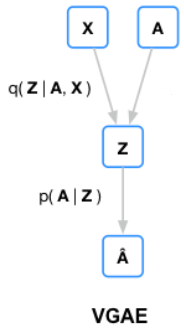
\includegraphics[width=.13\textwidth]{pics/VGAE.PNG}
	\caption{VGAE}
	\label{fig:vgae}
\end{figure}

\paragraph{VGAE思路}模型的思路如图Fig.\ref{fig:vgae}所示。其中$X \in \mathbb{R}^{N \times D}, A \in \mathbb{R}^{N \times N}$分别是无向图$G$的结点特征矩阵、邻接矩阵,$Z \in \mathbb{R}^{N \times F}$是$G$的隐表示,$\hat{A} \in \mathbb{R}^{N \times N}$是通过隐表示解码出的图的邻接矩阵,相当于根据隐表示重建后的图的邻接矩阵。整个模型可以看作一个VAE模型,分为编码和解码两个阶段。从$(X, A)$到$Z$通过GCN来完成,从$Z$到$\hat{A}$则是通过隐表示间的内积再通过激活函数得到边的概率。

\paragraph{方法解决的问题/优势}
\begin{itemize}
	\item 提出使用VAE模型对图进行编码和解码
	\item 在对图进行编/解码的过程中,隐表示$Z$可以视作结点表征

\end{itemize}

\paragraph{方法的局限性/未来方向}
\begin{itemize}
	\item 个人感觉编码过程略粗糙,不精细
	\item 扩展性不好
\end{itemize}

在看这篇论文之前,我以为这篇论文的重点是图的重建,但是文中更多地体现的是获得隐表示,将隐表示用于下游任务。那么,\tbc{red}{能否学习一个图编码器,能够很好地对图进行压缩,重建时又可能准确呢?}





\subsection{Rethinking pooling in graph neural networks}
\begin{center}

  \begin{tabular}{rp{16cm}lp{20cm}}%{rl}

  % after \\: \hline or \cline{col1-col2} \cline{col3-col4} ...

  论文地址:& \href{https://arxiv.org/pdf/2010.11418.pdf}{https://arxiv.org/pdf/2010.11418.pdf} \\
  来源:& NeurIPS, 2020 \\
  作者:& Diego Mesquita, Amauri H. Souza, Samuel Kaski \\

  %源码:& \href{xxx}{xxx} \\

%  slides:& \href{http://yunshengb.com/wp-content/uploads/2017/03/nips_2018_r2l_workshop_talk.pdf}{{\footnotesize Convolutional Set Matching for Graph Similarity}}\\

  关键词:& \textbf{GNN, Pooling} \\

  写于:& \date{2021-01-17}

  \end{tabular}

\end{center}

该论文\cite{mesquita2020rethinking}对GNN中常用的pooling操作进行了思考,pooling对GNN的性能有多大帮助?可谓是对很多论文中提出的各式各样的pooling打脸了啊。该论文选择了三种比较具有代表性的pooling进行研究,使用随机的操作替换原来的pooling,结果性能基本没有变化(\tbc{red}{尴尬}),之后作者分析了卷积与pooling之间的关系,解释了pooling不起作用的原因。


\paragraph{问题定义}
GNNs中的pooling与CNN中的pooling类似,一般都是为了下采样,减小输入的规模。GNNs中的pooling通过将graph中的结点聚合生成一个规模更小的graph --- 具有更少的结点数,结点特征也更少。大部分的GNNs中都用到了pooling(有些论文中也叫coarsening),也有一些论文专门提出了一些pooling操作。其实,graph的pooling可以视作一个对结点进行聚类的过程,给每个结点赋予一个类别,将同一类别的结点视作pooling后的graph中的一个结点,节点特征矩阵和邻接矩阵也会更具pooling结果进行调整。具体的pooling可以根据结点的特征进行聚类(通常做法),也可以用神经网络来学习学习聚类的结果。

既然大家都用pooling,它真的那么重要吗?

\paragraph{Rethinking思路}
作者选择了3个具有代表性的模型:GRACLUS\cite{dhillon2007weighted}、DIFFPOOL\cite{ying2019hierarchical}、GMN\cite{khasahmadi2020memory-based}。这3个模型里都使用了local pooling,作者对其中的pooling操作进行了修改,例如替换为随机的pooling、使用原graph的补graph进行pooling作为原graph的pooling结果等,在常用的数据集上对比了替换前后模型的效果。
惊人的事情出现了 --- 模型的效果基本没有变化,有些甚至不如替换后的效果好!!!

在分析阶段,作者主要分析了卷积和pooling对模型的影响。作者通过实验说明,卷积层学习到的结点特征是趋同的(同质的),而pooling则加重了这一现象,pooling可能会使得结点特征的方差变小。一个卷积相当于提取了一种特征,在实践中通常会使用多个卷积来提取特征。作者还实验了单个卷积和多个卷积对模型效果的影响 --- 单个卷积在大多数情况下效果都会比多个卷积更差,但是当特征是结点特征是常量是多个卷积对效果并无很大影响。卷积的数量与初始时结点特征的丰富程度有关。


\paragraph{方法解决的问题/优势}

\begin{itemize}
	\item 很大胆的质疑了几乎所有GNNs中都用到了pooling
	\item 在几个主流的pooling上进行了验证,与替换之后的pooling进行对比
	\item 分析了各种pooling效果甚微的原因,分析了卷积与pooling之间的联系

\end{itemize}


\paragraph{方法的局限性/未来方向}

\begin{itemize}
	\item pooling也许并不是没用的。论文只是替换了pooling,并没有取消pooling,\tbc{red}{或许具体的pooling没有那么重要,但不代表pooling不重要}
	\item 论文中所所验证的数据集都是规模比较小的graph,\tbc{red}{当扩展到规模大得多的graph上时,或许这个时候才能体现pooling的作用}
\end{itemize}

\subsection{FASTGCN: Fast Learning with Graph Convolutional Networks via Importance Sampling}
\begin{center}

  \begin{tabular}{rp{16cm}lp{20cm}}%{rl}

  % after \\: \hline or \cline{col1-col2} \cline{col3-col4} ...

  论文地址:& \href{https://arxiv.org/pdf/1801.10247.pdf}{https://arxiv.org/pdf/1801.10247.pdf} \\
  来源:& ICLR, 2018 \\
  作者:& Jie Chen, Tengfei Ma, Cao Xiao \\

  源码:& \href{https://github.com/matenure/FastGCN}{FastGCN} \\

%  slides:& \href{http://yunshengb.com/wp-content/uploads/2017/03/nips_2018_r2l_workshop_talk.pdf}{{\footnotesize Convolutional Set Matching for Graph Similarity}}\\

  关键词:& \textbf{GCN, GNN} \\

  写于:& \date{2021-01-21}

  \end{tabular}

\end{center}

该论文\cite{chen2018fastgcn}针对GCN训练和学习过程中地计算量大和耗时提出了integral transform的方法。本文所针对的Graph主要是稠密图和符合幂律的Graph,当对其中一个结点卷积时,所覆盖的结点集可能已经很大了。同时,FastGCN是inductive的。

本文的重点是对结点的采样以及从积分的角度来看待卷积层。

这篇论文没看太懂,可见博客:\href{https://zhuanlan.zhihu.com/p/106226258}{源码分析-FastGCN}、\href{https://blog.csdn.net/yyl424525/article/details/101101079}{FastGCN}。




\subsection{Contrastive and Generative Graph Convolutional Networks for Graph-based Semi-Supervised Learning}
\begin{center}

  \begin{tabular}{rp{16cm}lp{20cm}}%{rl}

  % after \\: \hline or \cline{col1-col2} \cline{col3-col4} ...

  论文地址:& \href{https://arxiv.org/pdf/2009.07111.pdf}{https://arxiv.org/pdf/2009.07111.pdf} \\
  来源:& AAAI, 2021\\
  作者:& Sheng Wan, Shirui Pan, Jian Yang, Chen Gong \\

  %源码:& \href{xxx}{xxx} \\

%  slides:& \href{http://yunshengb.com/wp-content/uploads/2017/03/nips_2018_r2l_workshop_talk.pdf}{{\footnotesize Convolutional Set Matching for Graph Similarity}}\\

  关键词:& \textbf{semi-supervised learning, GCN, Contrastive Learning} \\

  写于:& \date{2021-03-01}

  \end{tabular}

\end{center}

该论文\cite{wan2020contrastive}主要解决的是基于图的半监督学习中的监督信息短缺的问题,该论文结合数据之间的相似性和图结构来丰富监督信息。

\paragraph{问题定义}
假设共有$n=l+u$个样本(结点),$\Psi=\left\{\mathbf{x}_{1}, \cdots, \mathbf{x}_{l}, \mathbf{x}_{l+1}, \cdots, \mathbf{x}_{n}\right\}$,其中前$l$个样本为带标签的样本,标签为$\{y_i\}_{i=1}^l$,后$u$个样本不带标签,通常在半监督学习中$l$远小于$u$。特征矩阵为$\mathbf{X} \in \mathbb{R}^{n \times d}$,$\mathbf{Y} \in \mathbb{R}^{n \times c}$为标签矩阵。该论文的目标就是找到后$u$个结点的标签。(这是一个transductive的方法)。

\paragraph{思路}
\begin{figure}[h]
	\centering
	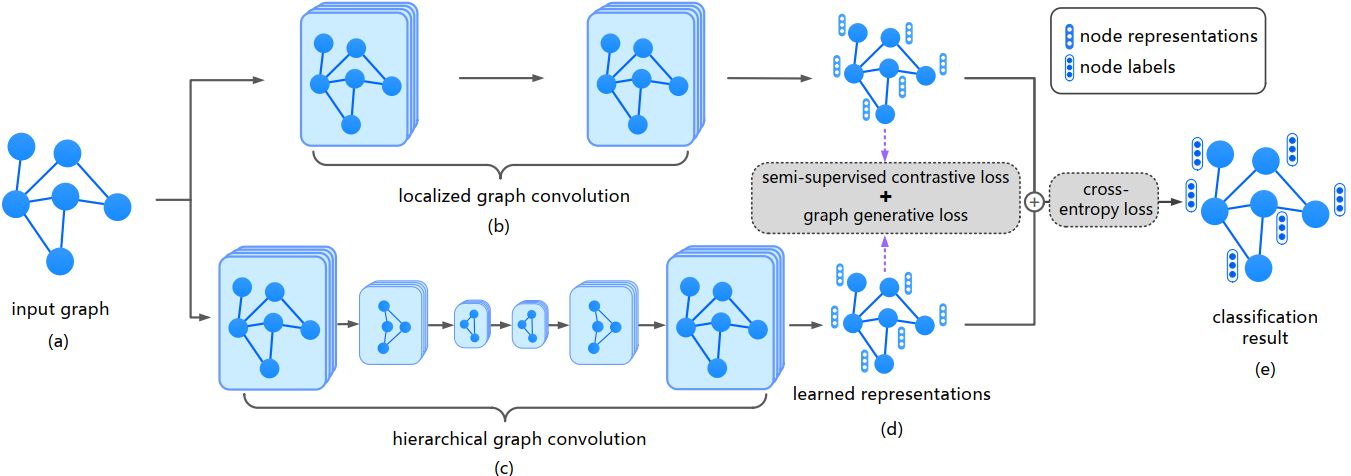
\includegraphics[width=.8\textwidth]{pics/CG3.png}
	\caption{CG3}
	\label{fig:cg3}
\end{figure}
整体框架如Fig.\ref{fig:cg3}所示。为了丰富监督信息,论文使用结点之间的相似性和图结构来丰富监督信息,分别使用半监督的对比学习来捕获数据之间的相似性和图生成损失来捕获图结构信息。

\subparagraph{Semi-Supervised Contrastive Learning}
对比学习通过数据之间的相似性与相异性来学习数据的表征,但是对比学习通常用在无标签数据中,不能利用标签数据。为此,论文中提出半监督的对比学习来利用带标签的数据。半监督的对比学习损失可以分为两部分:无监督的对比损失和监督的对比损失。

论文中使用local和global两种视角的GCN来生成结点表征(目的是为了后续的对比学习),分别表示为$\mathbf{H}^{\phi_1}, \mathbf{H}^{\phi_2}$。无监督的对比损失为:
$$
\mathcal{L}_{u c}=\frac{1}{2 n} \sum_{i=1}^{n}\left(\mathcal{L}_{u c}^{\phi_{1}}\left(\mathbf{x}_{i}\right)+\mathcal{L}_{u c}^{\phi_{2}}\left(\mathbf{x}_{i}\right)\right)
$$
其中$\mathcal{L}_{u c}^{\phi_{1}}\left(\mathbf{x}_{i}\right), \mathcal{L}_{u c}^{\phi_{2}}\left(\mathbf{x}_{i}\right)$分别为:
$$
\begin{array}{l}
\mathcal{L}_{u c}^{\phi_{1}}\left(\mathbf{x}_{i}\right)=-\log \frac{\exp \left(\left\langle\mathbf{h}_{i}^{\phi_{1}}, \mathbf{h}_{i}^{\phi_{2}}\right\rangle\right)}{\sum_{j=1}^{n} \exp \left(\left\langle\mathbf{h}_{i}^{\phi_{1}}, \mathbf{h}_{j}^{\phi_{2}}\right\rangle\right)}\\

\mathcal{L}_{u c}^{\phi_{2}}\left(\mathbf{x}_{i}\right)=-\log \frac{\exp \left(\left\langle\mathbf{h}_{i}^{\phi_{2}}, \mathbf{h}_{i}^{\phi_{1}}\right\rangle\right)}{\sum_{j=1}^{n} \exp \left(\left\langle\mathbf{h}_{i}^{\phi_{2}}, \mathbf{h}_{j}^{\phi_{1}}\right\rangle\right)}
\end{array}
$$

有监督的对比损失为:
$$
\mathcal{L}_{s c}=\frac{1}{2 l} \sum_{i=1}^{l}\left(\mathcal{L}_{s c}^{\phi_{1}}\left(\mathbf{x}_{i}\right)+\mathcal{L}_{s c}^{\phi_{2}}\left(\mathbf{x}_{i}\right)\right)
$$
其中$\mathcal{L}_{s c}^{\phi_{1}}\left(\mathbf{x}_{i}\right), \mathcal{L}_{s c}^{\phi_{2}}\left(\mathbf{x}_{i}\right)$分别为:
$$
\begin{array}{l}
	\mathcal{L}_{s c}^{\phi_{1}}\left(\mathbf{x}_{i}\right)=-\log \frac{\sum_{k=1}^{l} \mathbb{1}_{\left[y_{i}=y_{k}\right]} \exp \left(\left\langle\mathbf{h}_{i}^{\phi_{1}}, \mathbf{h}_{k}^{\phi_{2}}\right\rangle\right)}{\sum_{j=1}^{l} \exp \left(\left\langle\mathbf{h}_{i}^{\phi_{1}}, \mathbf{h}_{j}^{\phi_{2}}\right\rangle\right)} \\
	\mathcal{L}_{s c}^{\phi_{2}}\left(\mathbf{x}_{i}\right)=-\log \frac{\sum_{k=1}^{l} \mathbb{1}_{\left[y_{i}=y_{k}\right]} \exp \left(\left\langle\mathbf{h}_{i}^{\phi_{2}}, \mathbf{h}_{k}^{\phi_{1}}\right\rangle\right)}{\sum_{j=1}^{l} \exp \left(\left\langle\mathbf{h}_{i}^{\phi_{2}}, \mathbf{h}_{j}^{\phi_{1}}\right\rangle\right)},
\end{array}
$$

半监督对比损失为:$\mathcal{L}_{ssc} = \mathcal{L}_{uc} + \mathcal{L}_{sc}$。

\subparagraph{Graph Generative Loss}
为了利用图的结构作为监督信息引入了图生成损失。在现有生成模型的启示下,将图中边$e_{ij}$视为二元变量,并且该变量是条件独立的。所以在给定local和global视角的结点表征时,图的概率表示为:
$$
\begin{aligned}
	p(\mathcal{G} | \mathbf{H}^{\phi_1}, \mathbf{H}^{\phi_2}) = \prod_{i,j} p(e_{ij}| \mathbf{H}^{\phi_1}, \mathbf{H}^{\phi_2}) \\
	= \prod_{i,j} p(e_{ij}| \mathbf{h}_i^{\phi_1}, \mathbf{h}_j^{\phi_2}) \\
	= \prod_{i,j} \delta([\mathbf{h}_i^{\phi_1}, \mathbf{h}_j^{\phi_2}] \mathbb{w})
\end{aligned}
$$
(类似于极大似然概率),其中$\delta$为逻辑回归函数。

图生成损失为:$\mathcal{L}_{g^2} = - p(\mathcal{G} | \mathbf{H}^{\phi_1}, \mathbf{H}^{\phi_2})$。

\subparagraph{Model Training}
因为采用了local和global的视角,结点最终的表征为:$\mathbf{O} =f \lambda^{\phi_1}\mathbf{H}^{\phi_1} + (1-\lambda^{\phi_1})\mathbf{H}^{\phi_2}$。
因为还存在一部分带标签的数据,因此可以借助这一部分数据产生交叉熵损失:$\mathcal{L}_{ce} = -\sum_{i=1}^l \sum_{j=1}^c \mathbf{Y}_{ij} ln\mathbf{O}_{ij}$。
最终模型的损失即为:
$$
\mathcal{L} = \mathcal{L}_{ce} + \lambda_{ssc}\mathcal{L}_{ssc} + \lambda_{g^2}\mathcal{L}_{g^2}
$$
其中$\lambda_{ssc}, \lambda_{g^2}$均为超参数。

\paragraph{方法解决的问题/优势}

\begin{itemize}

	\item 将对比学习引入到半监督学习中,结合了不带标签的数据和带标签的数据
	\item 利用结点相似性与图结构来丰富监督信息

\end{itemize}



\paragraph{方法的局限性/未来方向}

\begin{itemize}

	\item 论文中的方法为transductive,不能应用于未见过的结点
	\item \tbc{red}{将论文中的方法改为inductive的}

\end{itemize}


\subsection{How powerful are graph gnns?}

\begin{center}
  \begin{tabular}{rl}
  % after \\: \hline or \cline{col1-col2} \cline{col3-col4} ...
  论文地址:& \href{https://arxiv.org/abs/1810.00826}{https://arxiv.org/abs/1810.00826} \\
  源码地址:& \href{https://github.com/weihua916/powerful-gnns}{powerful-gnns} \\
  关键词:& \textbf{GNN, WL graph isomorphism test} \\
  写于:& \date{2020-09-24}
  \end{tabular}
\end{center}

% \par 论文地址:\href{https://arxiv.org/abs/1810.00826}{https://arxiv.org/abs/1810.00826}
% \par GitHub地址:\href{https://github.com/weihua916/powerful-gnns}{powerful-gnns}
% \par 关键词:\textbf{GNN, WL graph isomorphism test}
% \par 写于:\date{2020-09-24}

论文\cite{xu2018how}对以往的GNN模型的表现能力(区分能力)进行了理论上的分析,主要针对不同aggregation 的特点进行了分析,并针对以往的GNNs的弱点,设计了GIN(graph isomorphism network),达到了与WL sub tree相匹配的性能。论文中使用两种分类任务对以往的GNNs和GIN, WL sub tree 进行了测试:结点分类、图分类。

论文由一个问题开始讨论GNNs的区分能力。\\
给定两个图$G_1, G_2$,不同的GNNs可能会将它们(或者两图中的某两个结点)嵌入到相同的表示。这是为什么呢?这就要讨论GNNs是如何来获得结点/图的embeddings了。考虑一个通用的GNN模型:
$$
h_v^{(k)} = COMBINE(h_v^{(k-1)},  AGGREGATE({h_u^{(k-1)} | u \in \mathcal{N}_v } ) )
$$
上式中的$AGGREGATE$用来聚集邻居结点的信息(如mean, max, GRU, LSTM, GAT等),$COMBINE$则用来将聚集后的邻居结点的信息与结点自身的信息进行组合(如拼接。其实这很像一个图中的消息传播模型,现有的很多GNN模型也是基于消息传播的方法来汇聚邻居结点的信息,k层的GNN 相当与汇聚了来自k-hop的邻居的信息。({\color{red}{能否使用其他的框架来构建GNN模型呢?}})对于图$G$的embedding,是由$G$中的所有结点形成的(这涉及graph embedding的问题,参见其他论文)。
$$
h_G = READOUT(h_v^{(K)} | v \in G)
$$
再回到论文中的问题:\textbf{以往的GNN可能无法区分某些结点/图,即对不同的结点/图不能生成唯一的embeddin,不是injective的!}。根据结点/图的embedding生成的方法可以看出,关键在于\\
$AGGREGATE, COMBINE, READOUT$,论文中将这些定义为 \textit{multi-set function},multi-set是一个可以有重复元素的集合,multi-set function就是定义在multi-set上的函数。问题就出在了GNNs使用的某些multi-set function上!
\par 论文主要对不同的AGGREGATE进行了分析,且主要分析了mean, max两种方法。
\begin{figure}[h]
    \centering
    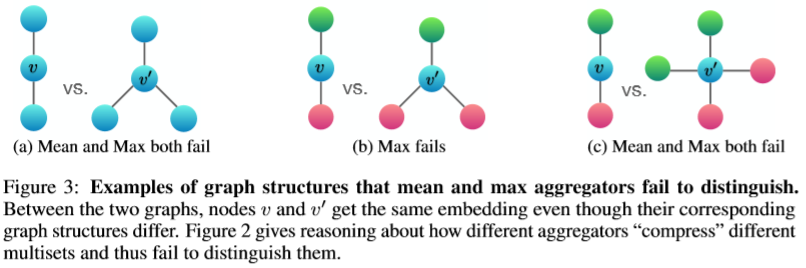
\includegraphics[width=1.\textwidth]{pics/mean-max.png}
    \caption{令Mean, Max失败的例子}
    %\label{fig:my_label}
\end{figure}
如上图所示,展示了mean, max 无法区分两个图中不同结点的邻居情况(neighborhood,即AGGREGATE后的结果是一样的)。论文中分别对mean, max的特性进行了阐述。\\
先给一个形式化的定义,假设$X$为某个结点的邻居结点集,$h(X)$就是AGGREGATE。
\paragraph{MEAN Learns Distributions} 当$h(X) = \frac{1}{|X|}\sum_{x\in X} f(x)$ 时,若对于不同的邻居结点集$X_1, X_2$,若$h(X_1) = h(X_2)$,则$X_1$和$X_2$有着相同的分布。从统计意义上来理解,相当于两个分布的均值(mean)相同。所以,当我们更需要捕捉图中某种信息的分布或者信息重复较少时,mean会有不错的效果。

\paragraph{MAX Identity "Skeleton"}(妙!) 当$h(X) = max_{x\in X}f(x)$时,若对于不同的$X_1, X_2$有$h(X_1) = h(X_2)$,则$X_1$和$X_2$有着相同的underlying set。当使用max作为AGGREGATE时,相当于对multi-set中的“重点”元素进行关注,当放在整个图中看时,相当于抽取了图中某种意义上比较“强”的结点。

\par 接下来就是重头戏 --- GIN了。
\par 论文中对结点和图的GIN定义如下:
$$
h_v^{(k)} = MLP^{(k)} ((1+\epsilon^{(k)} ) \cdot h_v^{(k-1)}+\sum_{u \in \mathcal{N}(v)} h_u^{(k-1)} ))  \newline
$$
$$
h_G = CONCAT(READOUT({h_v^{(k)} | v \in G}) | k = 0,1,...,K)
$$
看到上面的定义,你可能会疑惑,为什么GIN就比其他的GNNs好呢?这和以往的GNNs有什么区别呢?论文中对GIN使用的AGGREGATE进行了理论上的证明,证明GIN是injective的。
\par 论文中通过两个结论证明了GIN的injective性。说了几次injective了,那什么是injective呢?\\
\textbf{injective function}: 定义域中的每个不同的原像在值域中的像都是唯一的。
那么,为了让GNN有足够powerful的表现/识别能力,GNN需要尽可能精确地区分每个不同的结点/图(GNN作为以一种主要的embedding方法,高精度的表示能力能为下游任务打好基础),所以应尽量使AGGREGATE, COMMBINE, READOUT 是injective的。\\
{\color{red}证明GIN的injective}

\par 再来谈一下  Weisfeiler-Lehman (WL) graph isomorphism test 。WL isomorphism test 是用来比较两个图是否是同构的。先解释一下同构的概念。\\
抛开图同构,把同构概念单独拎出来看。对于两个系统中的对象,同构映射能够保持两个系统中的对象一一对应,且对象之间的关系也能够一一对应。图同构中,$v_1 = f(u_1), v_2 = f(u_2),u_1, u_2 \in G_1, v_1, v_2 \in G_2$,若$u_1, u_2$之间有边,则$(v_1, v_2) = g((u_1, u_2))$。\\
WL test 是通过迭代的聚集邻居的标签,每次迭代后将自己的标签和邻居们的标签映射成一个新的标签(相当于AGGREGATE后在COMBINE),迭代完成后比较两个图的标签分布(简单来说即各个标签分别有几个)是否一致({\color{red}结点的标签能否收敛呢?为什么标签的分布能用来判定是否同构呢?}),如果标签分布一致,则两个图可能是同构的。
WL subtree kernel\cite{shervashidze2011weisfeiler} 是基于 WL test的。我并没有通读论文,但是粗略看了一下图,感觉 WL subtree kernel和现在的GNN已经很像了, 对于每个结点,WL subtree kernel构建以该结点为root的树,子节点为其邻居结点,子节点的子节点是邻居结点,如此循环定义,最后以这颗树作为结点标签的依据。WL subtree kernel是目前基于聚合方式的GNNs的性能上界(证明见论文appendix)。但是WL subtree kernel并不能结合结点的信息,对于现在图中结点丰富的信息来说,这不免是有点浪费的,而且,个人认为WL subtree kernel捕捉的是图的结构(毕竟是衍生于图同构算法),或许图中的其他信息它是没有捕捉到的({\color{red}是什么信息呢?}) 

\par 关于未来的研究方向。有没有比基于聚集邻居结点信息(信息传递)方法更好的一个GNN框架呢?

关于WL test可参考的博客/非文献资料:
\begin{enumerate}
    \item \href{https://www.davidbieber.com/post/2019-05-10-weisfeiler-lehman-isomorphism-test/}{The Weisfeiler-Lehman Isomorphism Test}
\end{enumerate}


\subsection{Inductive and Unsupervised Representation Learning on Graph Structured Objects}
\begin{center}

  \begin{tabular}{rp{16cm}lp{20cm}}%{rl}

  % after \\: \hline or \cline{col1-col2} \cline{col3-col4} ...

  论文地址:& \href{https://openreview.net/pdf?id=rkem91rtDB}{https://openreview.net/pdf?id=rkem91rtDB} \\
  来源:& ICLR, 2020 \\
  作者:& Lichen Wang, Bo Zong, et al. \\
  源码:& \href{https://github.com/wenwen0319/SEED-Reimplementation}{SEED-Reimplementation} \\
  slides:& \href{https://github.com/wanglichenxj/Inductive-and-Unsupervised-Representation-Learning-on-Graph-Structured-Objects/blob/master/presentations/ICLR_slides.pdf}{{\footnotesize SEED}}\\
  关键词:& \textbf{unsupervised learning, graph representation} \\
  写于:& \date{2021-03-01}
  \end{tabular}
\end{center}

该论文\cite{SEED_Lichen}主要解决的是图结构数据的无监督的、inductive形式的表征问题。通常在无监督的图表征问题中,主要以重建损失为主导进行训练,但是在计算重建损失时通常要涉及到图的相似性计算,而图的相似性计算是一个十分复杂、耗时的过程,论文提出了一个通用的框架SEED(Sampling, Encoding and Embedding Distribution)用于无监督的学习图结构对象的表征。

\paragraph{问题定义}
目标很简单,给定一个graph,学习它的表征。

\paragraph{SEED思路}
\begin{figure}[h]
	\centering
	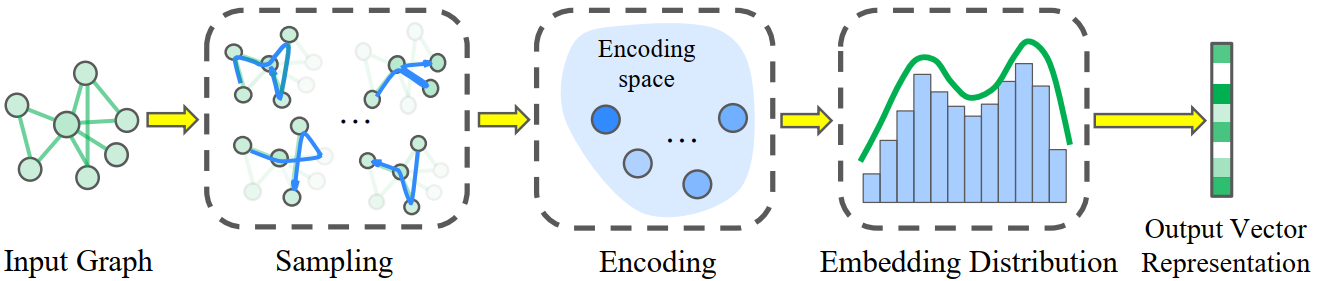
\includegraphics[width=.8\textwidth]{pics/SEED.png}
	\caption{SEED}
	\label{fig:seed}
\end{figure}
如Fig.\ref{fig:seed}所示,SEED主要分为三个部分:
\subparagraph{Sampling}
从输入的图中采样出多个子图。为了使得采样到的子图更具代表性,论文中提出了一种新的采样方法 --- WEAVE(random Walk with EArliest Visit timE)。该方法与通常的随机游走不一样,WEAVE是带结点访问时间戳的。
\begin{figure}[h]
	\centering
	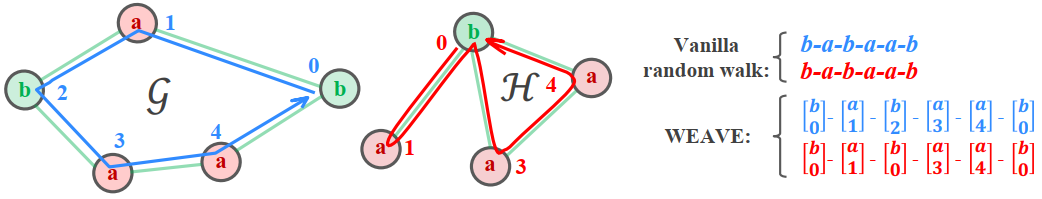
\includegraphics[width=.8\textwidth]{pics/WEAVE.png}
	\caption{WEAVE与随机游走对比}
	\label{fig:weave}
\end{figure}
如Fig.\ref{fig:weave}所示,WEAVE的区分能力比平凡的搜集游走更强。每一个WEAVE都代表一个采样到的子图,可以用一个矩阵表示:$X=\left[\mathbf{x}^{(0)}, \mathbf{x}^{(1)}, \cdots, \mathbf{x}^{(k)}\right]$,其中$\mathbf{x}^{(p)} = [\mathbf{x}_a^{(p)}, \mathbf{x}_t^{(p)}]$,$\mathbf{x}_a^{(p)}$表示在时间$p$时访问到的结点的特征,$\mathbf{x}_t^{(p)}$表示访问到该结点时的时间向量。\tbc{red}{注意,如果访问到了已经访问过的结点则$\mathbf{x}_t^{(p)}$为最早访问时的时间}。在论文中,$\mathbf{x}_t^{(p)}$采用one-hot编码。

\subparagraph{Encoding}
将每一个采样到的子图编码为向量。直觉上,如果子图的表征质量好,那么就能在子图表征地基础上较好地重建子图。论文中作者采样自编码器学习子图的表征,以重建损失作为损失函数。至此,$s$个子图$\{X_1, ..., X_s\}$被表示为$s$个向量$\{\mathbf{z}_1, ..., \mathbf{z}_s\}$。

\subparagraph{Embedding Distribution}
将上一阶段获得的多个子图的表征汇集作为输入图的表征。对于两个图,它们在表征空间中的距离应该与它们的子图向量分布距离类似,因此需要找到一个好的聚集函数来保留原先的子图表征分布距离,论文中采用的是$MMD$。
给定连个图$\mathcal{G}, \mathcal{H}$,子图表征分别为:$\{\mathbf{z}_1, ..., \mathbf{z}_s\}$和$\{\mathbf{h}_1, ..., \mathbf{h}_s\}$,则两者间的$MMD$为:
$$
\begin{aligned}
	\widehat{M M D}\left(P_{\mathcal{G}}, P_{\mathcal{H}}\right)=& \frac{1}{s(s-1)} \sum_{i=1}^{s} \sum_{j \neq i}^{s} k\left(\mathbf{z}_{i}, \mathbf{z}_{j}\right)+\frac{1}{s(s-1)} \sum_{i=1}^{s} \sum_{j \neq i}^{s} k\left(\mathbf{h}_{i}, \mathbf{h}_{j}\right) \\
	&-\frac{2}{s^{2}} \sum_{i=1}^{s} \sum_{j=1}^{s} k\left(\mathbf{z}_{i}, \mathbf{h}_{j}\right) \\
	=&\left\|\hat{\mu}_{\mathcal{G}}-\hat{\mu}_{\mathcal{H}}\right\|_{2}^{2}
\end{aligned}
$$
$\hat{\mu}_{\mathcal{G}}, \hat{\mu}_{\mathcal{H}}$分别表示两个图的kernel embedding,也就是最终的graph representation,分别定义为:
$$
\hat{\mu}_{\mathcal{G}}=\frac{1}{s} \sum_{i=1}^{s} \phi\left(\mathbf{z}_{i}\right), \quad \hat{\mu}_{\mathcal{H}}=\frac{1}{s} \sum_{i=1}^{s} \phi\left(\mathbf{h}_{i}\right)
$$
其中$\phi(\cdot)$是与核函数$k(\cdot, \cdot)$相关的特征映射函数(与SVM中的核技巧类似,将核函数的计算转化为更简单的计算形式)。
根据核函数的选择,$\phi(\cdot)$具有不同的形式,如RBF、MLP等。为了训练$\phi(\cdot)$,文中使用如下的近似误差,其中$\theta_m$为$\phi(\cdot)$的参数):
$$
J\left(\theta_{m}\right)=\left\|D\left(P_{\mathcal{G}}, P_{\mathcal{H}}\right)-\widehat{M M D}\left(P_{\mathcal{G}}, P_{\mathcal{H}}\right)\right\|_{2}^{2}
$$
通过最小化上述误差,就能学习到较好的聚集函数,在最终的表征中保留子图表征的分布距离。

该论文的方法与核方法有一定的相似性。论文还证明了同构的图的WEAVE的子图分布是类似的,并且对子图的采样长度进行了证明,详细内容可以参考论文。

\paragraph{方法解决的问题/优势}

\begin{itemize}

	\item 给出了无监督形式的、inductive的图结构对象表征学习方法
	\item 避免了复杂的图相似性计算,以类似于核技巧的方法较好地度量了图之间地距离
	\item 对相关地定理进行了证明

\end{itemize}



\paragraph{方法的局限性/未来方向}

\begin{itemize}

	\item 当图地规模较大时,采样的子图也会非常大,且可能需要采样地子图数量会很大

\end{itemize}

\subsection{DeepGCNs: Can GCNs Go as Deep as CNNs?}
\begin{center}

  \begin{tabular}{rp{16cm}lp{20cm}}%{rl}

  % after \\: \hline or \cline{col1-col2} \cline{col3-col4} ...

  论文地址:& \href{https://arxiv.org/pdf/1904.03751.pdf}{https://arxiv.org/pdf/1904.03751.pdf} \\
  来源:& ICCV, 2019\\
  作者:& Guohao Li, Matthias Muller, et al \\

  源码:& \href{https://github.com/lightaime/deep_gcns_torch}{deep\_gcns\_torch} \\

%  slides:& \href{http://yunshengb.com/wp-content/uploads/2017/03/nips_2018_r2l_workshop_talk.pdf}{{\footnotesize Convolutional Set Matching for Graph Similarity}}\\

  关键词:& \textbf{GCN, Point Cloud Segmentation} \\

  写于:& \date{2021-03-16}

  \end{tabular}

\end{center}

该论文\cite{li2019deepgcns}聚焦于深度GCN的训练及在点云数据上的分割问题。常见的GCN的层数都比较少,相关研究表明深层的GCN可能会引起如下问题:
\begin{itemize}
	\item over-smothing,一个连通分量内的结点的表征会趋同
	\item 较高的复杂度,不利于反向传播
	\item 梯度消失
\end{itemize}
该论文将CNN中的一些技巧引入深层GCN模型的构建,并将其应用在点云数据分割上。

\paragraph{问题定义}
\begin{figure}[h]
	\centering
	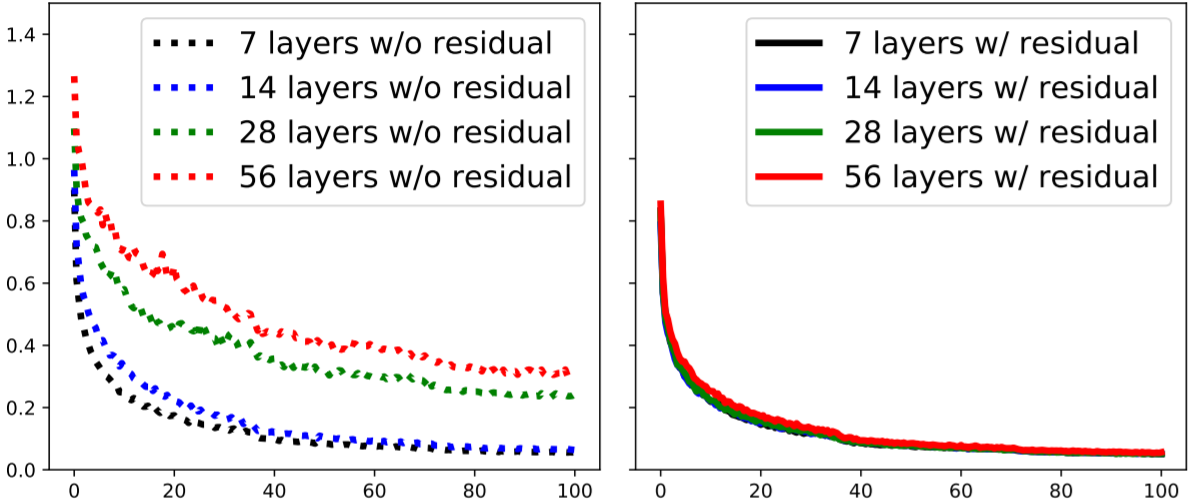
\includegraphics[width=.8\textwidth]{pics/Training-deep-GCNs.png}
	\caption{Traing deep GCNs}
	\label{fig:traing_deep_gcns}
\end{figure}
如Fig.\ref{fig:traing_deep_gcns}所示,当GCN的深度增加后,模型的损失并没有降低,这与\cite{he2016deep}中的模型退化现象很相似。怎么才可以让GCN像CNN一样,能够搭建出很深的模型呢?

\paragraph{DeepGCN}
作者从CNN中引入了三个技巧来解决这个问题:1)Residual learning;2)Dense Connection;3)Dilated Aggregation。

\subparagraph{Residual Learning for GCNs}
单纯地堆积卷积层对GCN地效果并没有很大的提升,其中一个原因可能是随着深度的增加,梯度难以反向传播,阻碍了模型的学习。Residual Learning的引入就是为了解决这个问题。
与Residual类似,如果原本要学习的映射为$\mathcal{H}$,残差的映射为$\mathcal{F}$,则残差学习表示如下:
$$
\begin{aligned}
	\mathcal{G}_{l+1} &= \mathcal{H}(\mathcal{G}_l, W_l)	\\
					  &= \mathcal{F}(\mathcal{G}_l, W_l) + \mathcal{G}_l = \mathcal{G}_{l+1}^{res} + \mathcal{G}_l
\end{aligned}
$$
第$l$层的输出经过$\mathcal{F}$的转换再与第$l$层的输出逐个顶点(vertex-wise)相加得到第$l+1$层的输出。

\subparagraph{Dense Connections in GCNs}
DenseNet的提出是为了利用层之间的稠密连接,提高网络中信息的流动,能够对层之间的特征进行重用,形式如下:
$$
\begin{aligned}
	\mathcal{G}_{l+1} &= \mathcal{H}(\mathcal{G}_l, W_l) \\
	  				  &= \mathcal{T}(\mathcal{F}(\mathcal{G}_l, W_l), \mathcal{G}_l) \\
	  				  &= \mathcal{T}(\mathcal{F}(\mathcal{G}_l, W_l), ..., \mathcal{F}(\mathcal{G}_0, W_0), \mathcal{G}_0)
\end{aligned}
$$
其中$\mathcal{T}$是一个逐顶点的连接操作,将输入的graph的结点的特征与中间各个GCN层的输出进行拼接。


\subparagraph{Dilated Aggregation inn GCNs}
空洞卷积弥补了pooling操作对空间信息的损失,在增大感受野的同时保留了位置信息。在改论文中,作者使用Dilated Aggregation来为每个结点聚集信息,以论文中进行的点云分割实验为例 --- 使用Dilated k-NN为每个顶点生成它的邻居。在每个GCN层后,作者使用Dilated k-NN来为每个顶点生成$k$个邻居,这$k$个邻居是从与这个顶点距离最近的$k \times d$个顶点以步长为$d$选择出来的,即顶点$v$的邻居为:$\mathcal{N}^{(d)}(v) = \{u_1, u_{1+d}, u_{1+2d}, ..., u_{1+(k-1)d}\}$。如Fig.\ref{fig:dilated_convolution_in_gcns}所示,上部分为dilated卷积,下部分为dilated k-NN,其中选择的$d$分别为1,2,4。在实践中,作者还增加了一点随机性,以$\epsilon$的概率随机从$k \times d$中选择$k$个顶点。

\begin{figure}[h]
	\centering
	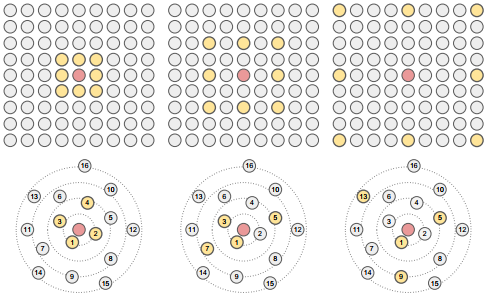
\includegraphics[width=.6\textwidth]{pics/Dilated-Convolution-in-GCNs.png}
	\caption{Dilated Convolution in  GCNs}
	\label{figz:dilated_convolution_in_gcns}
\end{figure}

最终,论文中用于点云数据分割的深度GCN架构如Fig.\ref{fig:deepgcn}所示。其中的区别为GCN Backbone Block,这个block有三个选择:1)普通的GCN;2)ResGCN;3)DenseGCN。
\begin{figure}[h]
	\centering
	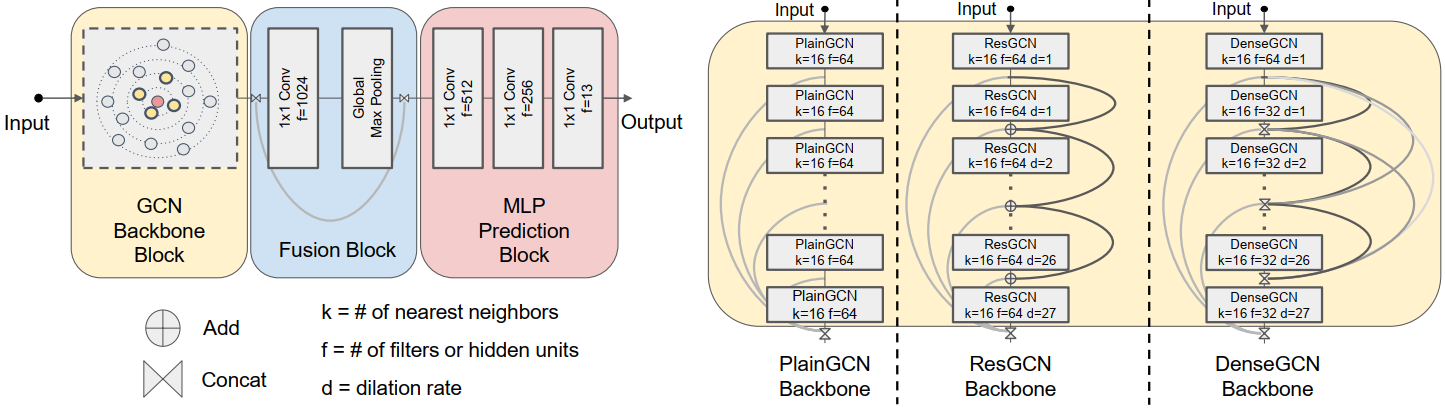
\includegraphics[width=.85\textwidth]{pics/DeepGCN.png}
	\caption{DeepGCN}
	\label{figz:deepgcn}
\end{figure}

\paragraph{总结}

\begin{itemize}

	\item 将CNN中的技术引入到GCN中,使得训练深层的GCN模型称为可能
	\item 将GCN应用于点云数据分割

\end{itemize}


%\paragraph{方法的局限性/未来方向}

%\begin{itemize}

%	\item 

%\end{itemize}






\subsection{Gated Graph Sequence Neural Networks}
\begin{center}
  \begin{tabular}{rl}
  % after \\: \hline or \cline{col1-col2} \cline{col3-col4} ...
  论文地址:& \href{https://arxiv.org/abs/1511.05493}{https://arxiv.org/abs/1511.05493} \\
  源码地址:& \href{https://github.com/yujiali/ggnn}{ggnn} (coded in Lua) \\
  slides:& \href{http://www.cs.toronto.edu/~yujiali/files/talks/iclr16_ggnn_talk.pdf}{ggnn-talk}\\
  关键词:& \textbf{RNN, Graph Sequential tasks} \\
  写于:& \date{2020-09-28}
  \end{tabular}
\end{center}

这篇论文\cite{li2015gated}提出了一种基于GRU\cite{cho2014learning}的GNN,能够进行输出单个值的任务(如结点分类、图分类等),也能完成\textbf{序列输出}的任务(如最短路、欧拉环等)。论文中使用bAbI\cite{weston2015aicomplete}(bAbI是Facebook AI推出的文本理解/推理任务生成器)任务和程序验证的任务对GG-NN, GGS-NN进行了测试均达到了很好的效果。
\par 论文中讨论的是针对有向图的GNN。那么是如何表示有向图的GNN呢?\\
对于有向图$\mathcal{G} = (\mathcal{V}, \mathcal{E})$,其邻接矩阵由两部分组成$A=[A_{in}, A_{out}]$,$A_{in},A_{out}$分别为入,出邻接矩阵。$\mathcal{G}$中每个结点$v$都定义了其$IN$和$OUT$结点集,分别表示指向$v$的边的起始结点集和从$v$出发的边的终点结点集。$v$的邻居结点集$NBR$定义为$IN \cup OUT$,并且对于边和结点都可以有各自的标签。
\par 论文中对GNN进行了回顾。GNN将图数据映射到输出的过程中,可以划分为两个部分:PROPAGATION MODEL, OUTPUT MODEL,分别用来计算节点的表征和将节点表征映射到输出。
\par 论文针对非序列的输出和序列的输出分别提出了GG-NNs(Gated Graph Neural Networks)和GGS-NNs(Gated Graph Sequence Neural Networks)。其中GG-NNs是基于GNN的,不同的是使用了GRU来构建PROPAGATION MODEL 和 OUTPUT MODEL。用于输出序列的GGS-NN则是在GG-NN的基础上构建的。接下来先介绍一下GRU\cite{cho2014learning},在介绍GG-NN和GGS-NN。
\paragraph{GRU(Gated Recurrent Unit)} 门控循环单元。GRU可以视为LSTM的变体,与LSTM很相似。与常规的RNN中的单元相比,门控神经单元间的连接是不变的,但每个门控神经单元内部都是经过精心设计的。作为门控RNN能够学会决定何时清除状态。
\begin{figure}[h]
    \centering
    \subfigure[LSTM cell]{
        \label{fig:lstm_cell}
        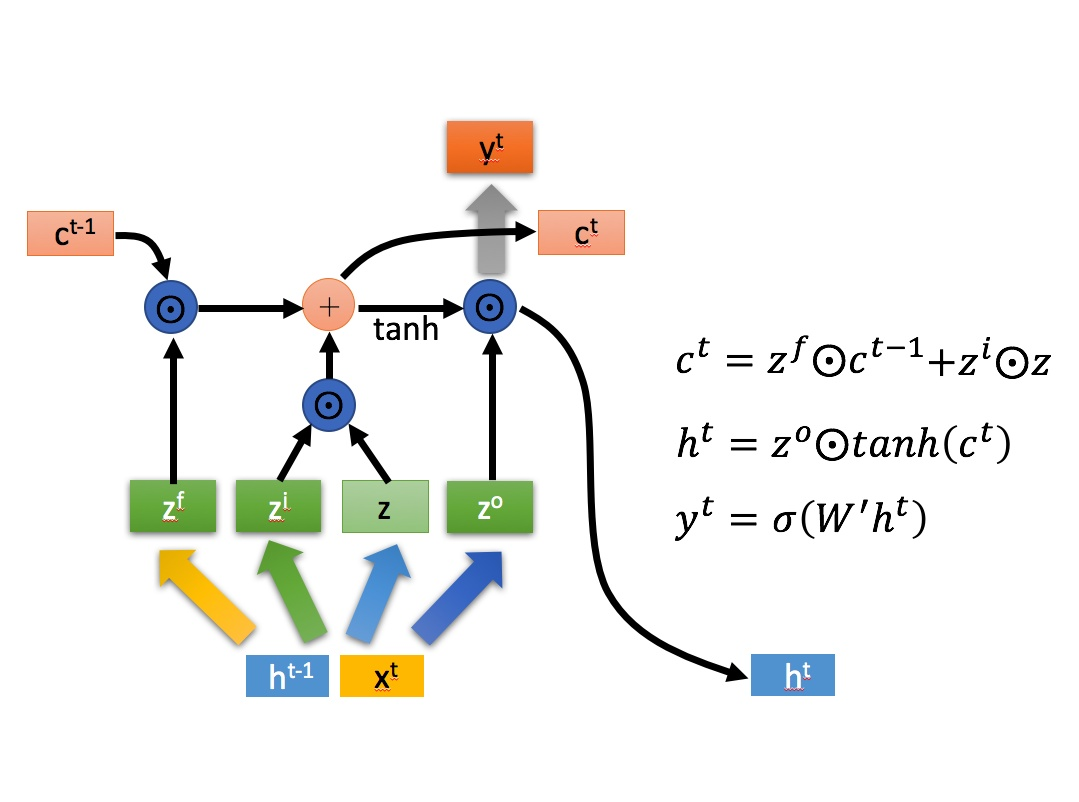
\includegraphics[width=.57\textwidth]{pics/LSTM.jpg}}
    \hspace{1.5pt}
    \subfigure[GRU cell]{
        \label{fig:gru_cell}
        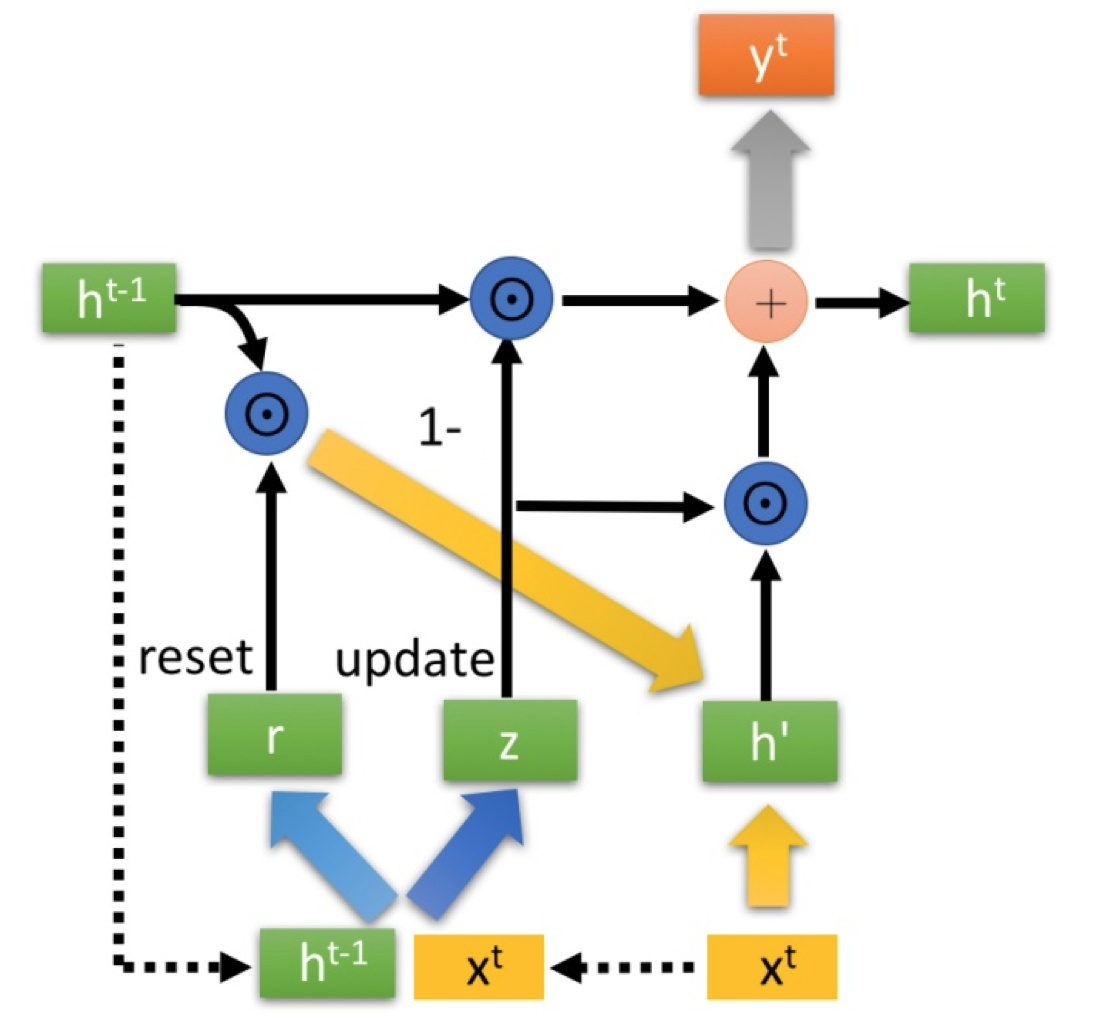
\includegraphics[width=.4\textwidth]{pics/GRU.jpg}}
    \caption{LSTM 和 GRU cell的内部结构}
    \label{fig:cell}
\end{figure}

\paragraph{GG-NN} GG-NN 的过程如下图所示。
\begin{figure}[h]
    \centering
    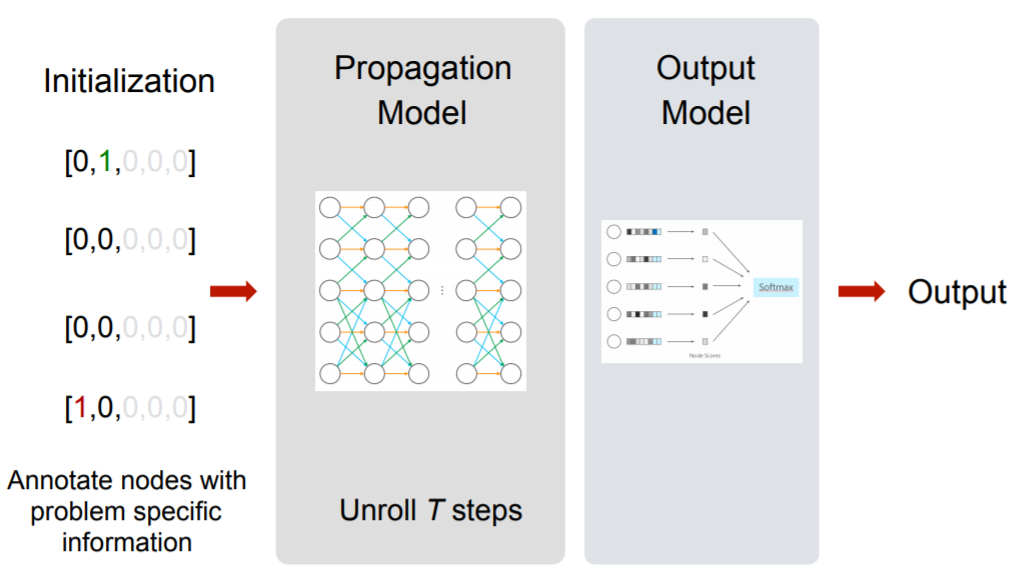
\includegraphics[width=.66\textwidth]{pics/ggnn.png}
    \caption{GG-NN}
    \label{fig:gg-nn}
\end{figure}
从Fig.\ref{fig:gg-nn}中可以看出,GG-NN的输入是 "Annotate nodes with problem specific information",在论文中称为"Node Annotations",这与之前提到的结点标签并不是同一个,node annotations 是在特定问题下所定义的“标签/特征”。根据特定的问题领域会为每个节点生成annotation({\color{red}如何生成annotations?}),在输入层会将annotation用0填充成固定的大小作为网络的输入。结点的annotations通过PROPAGATION MODEL---基于GRU的t层({\color{red}论文中成t-steps, 但根据我的理解是指网络有t层})网络,再将计算后的数据通过OUTPUT MODEL输出任务结果。

\paragraph{GGS-NN} GGS-NN 的过程如下。
\begin{figure}[h]
    \centering
    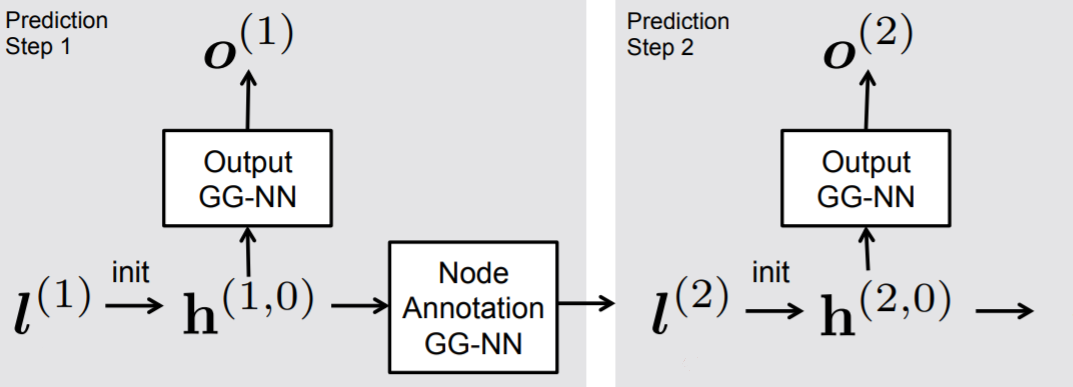
\includegraphics[width=.6\textwidth]{pics/GGS-NN.png}
    \caption{GGS-NN}
    \label{fig:ggs-nn}
\end{figure}
从Fig.\ref{fig:ggs-nn}中也能看出,GGS-NN是在GG-NN的基础上搭建的。GGS-NN的输入也是Node Annotations。每一步输入的Annotations是根据上一步的的隐层的输出转换而来的。每一步中的隐层输出会分别传给两个GG-NN,一个用来产生这一步的输出,另一个则用来产生下一步的输入,即下一步输入的node annotations。其实,在GGS-NN中除了上述两个GG-NN外,还有一个GG-NN用于在每一步确定是否继续,该GG-NN会在graph-level(把图看成一个特殊的结点,与图中的所有结点都有联系)上来进行一个二分类。

\par 论文中使用bAbI任务和程序逻辑验证进行测试。bAbI任务中将实体和实体间关系看作点和边(有点类似知识图谱),利用GG-NN/GGS-NN来进行推理。为解决程序验证中的program invariants 问题是这篇论文的一个主要出发点。通过将程序运行过程中heap的状态看作图数据,在这些数据的基础上以序列的方式生成程序的sepration logic\cite{10.1007/3-540-44802-0_1} 表达式。
\newline
网络参考资料:
\begin{enumerate}
    \item \href{https://www.jiqizhixin.com/articles/2017-12-24}{门控循环单元(GRU)的基本概念与原理}
    \item \href{https://towardsdatascience.com/illustrated-guide-to-lstms-and-gru-s-a-step-by-step-explanation-44e9eb85bf21}{Illustrated Guide to LSTM’s and GRU’s: A step by step explanation}
\end{enumerate}






\subsection{On the Bottleneck of Graph Neural Networks And Practical Implcation}
\begin{center}

  \begin{tabular}{rp{16cm}lp{20cm}}%{rl}

  % after \\: \hline or \cline{col1-col2} \cline{col3-col4} ...

  论文地址:& \href{https://openreview.net/pdf?id=i80OPhOCVH2}{https://openreview.net/pdf?id=i80OPhOCVH2} \\
  来源:& ICLR, 2021 \\
  作者:& Uri Alon, Eran Yahav \\

  源码:& \href{https://github.com/tech-srl/bottleneck/}{bottleneck} \\

%  slides:& \href{http://yunshengb.com/wp-content/uploads/2017/03/nips_2018_r2l_workshop_talk.pdf}{{\footnotesize Convolutional Set Matching for Graph Similarity}}\\

  关键词:& \textbf{GNN, Over-Squashing} \\

  写于:& \date{2021-03-28}

  \end{tabular}

\end{center}

该论文\cite{alon2021on}针对GNN中的远距离信息的传播问题提出了一个新的解释。文中讨论的问题是:GNN在聚集/利用远距离结点的信息时存在困难/一个瓶颈。论文针对这个问题进行了讨论和分析,并通过一些例子验证了这个问题。

\paragraph{Over Suqashing}
\begin{figure}[h]
	\centering
	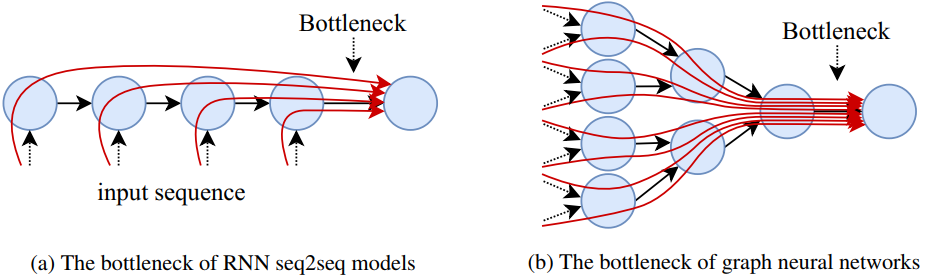
\includegraphics[width=.9\textwidth]{pics/bottleneck.png}
	\caption{The bottlenecks of Seq2seq and GNN models}
	\label{fig:bottleneck}
\end{figure}
作者将这个Bottleneck称为Over Suqashing,如Fig.\ref{fig:bottleneck}所示。什么是Over Squashing 呢?这就要从GNN的工作方式开始说起了。

GNN的工作方式是不断的将邻居结点的信息汇集(aggregate)起来,再进行后续的操作,通常一层汇聚的就是1-hop的邻居的信息,k层就可以汇聚到k-hop邻居的信息。随着层数的增加,一个结点的k-hop邻居的数量将会呈指数的形式增长,但是与前几层相比,更多的信息被压缩到了一个定长的向量中,这就是 over squashing。

在一些graph的任务中,不仅需要依靠局部的信息,如1-hop或者比较近的邻居的信息,同时还需要远距离的结点的信息。作者对任务所需要的邻居结点的距离定义为\textit{problem radius}。目前大部分使用的GNN都是比较浅层的,比如GCN的开山之作中就只有两层。作者在实验中还发现GCN、GIN比GAT等一些GNN模型更容易出现这个问题,显然,注意力机制在这里起了作用。

over squashing是指随着层数增加,指数速度增加的邻居的信息被过度压缩进了一个定长向量中,还有一个问题就是,对于最短路径大于GNN层数的情况,这个时候远距离的结点信息就不能传过来了,作者将其定义为under reaching。

作者在实验中发现,当\textit{problem radius}越大,则结点表征就需要更大的维度。

\paragraph{总结}

\begin{itemize}

	\item 将详细地研究了GNN中的远距离结点的信息的传播问题
	\item 之前的一些工作与这个有关,如\cite{li2019deepgcns}
	\item 有哪些较好地方法可以解决over squashing问题呢?
	\item 对于远距离结点地信息传播问题,能否通过在汇聚邻居信息时,随机采样较远的结点,作为远距离结点信息地补充
	\item 有哪些任务是需要远距离结点信息的呢?
	\item 能否用Transformer来作为GCN中的aggregate操作?

\end{itemize}



\subsection{Hierarchical Graph Representation Learning with Differentiable Pooling}
\begin{center}

  \begin{tabular}{rp{6cm}lp{12cm}}%{rl}

  % after \\: \hline or \cline{col1-col2} \cline{col3-col4} ...

  论文地址:& \href{https://arxiv.org/abs/1806.08804}{https://arxiv.org/abs/1806.08804} \\

  源码:& \href{https://github.com/RexYing/diffpool}{diffpool} \\

%  slides:& \href{http://yunshengb.com/wp-content/uploads/2017/03/nips_2018_r2l_workshop_talk.pdf}{{\footnotesize Convolutional Set Matching for Graph Similarity}}\\

  关键词:& \textbf{GNN, Graph Classification, Graph Pooling} \\

  写于:& \date{2020-10-21}

  \end{tabular}

\end{center}

该论文\cite{ying2019hierarchical}解决的是图分类的问题,针对之前的图分类中没有利用层次化的图的信息,提出了DIFFPOOL(Differentiable Pooling) --- 一种图池化(graph pooling)的方法,能够生成层次化的图的表示。DIFFPOOL的思路在GNN的基础上,学习软聚类分配(soft cluster assignment)的矩阵,将每个结点分配到不同簇中形成一个新的图,在新的图上继续使用GNN和DIFFPOOL来得到图层次化的表示,最终图将池化为一个点,使用这个点的表征进行分类。

\begin{figure}[h]
	\centering
	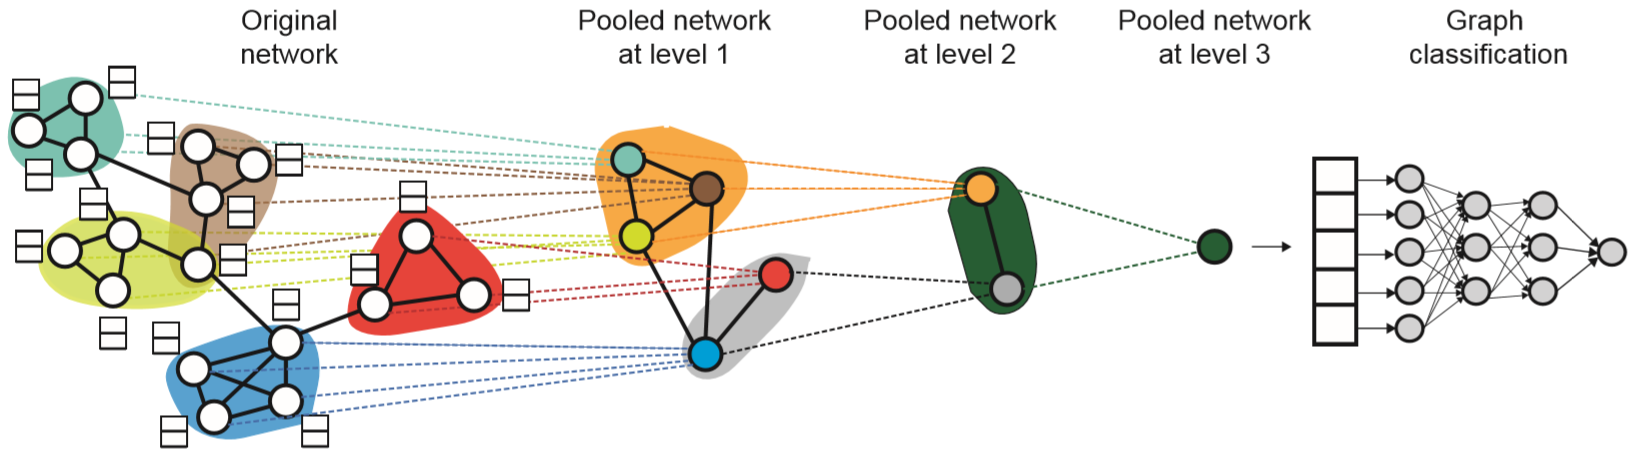
\includegraphics[width=.8\textwidth]{pics/DIFFPOOL.PNG}
	\caption{Overview of DIFFPOOL}
	\label{fig:diffpool}
\end{figure}

\paragraph{DIFFPOOL思路}DIFFPOOL的过程如Fig.\ref{fig:diffpool}所示。通过逐步将图中的结点压缩成一个节点,形成新的图的方法,逐步得到图的多个层次化的表示,最终图将被压缩成一个结点,再将这个结点的表征输入MLP中对图进行分类。为了得到图的结点表征和对图中结点进行软聚类,DIFFPOOL中一共用到了两个GNN,$GNN_{embed}$用于学习图的结点表征,$GNN_{pool}$用于学习软分配矩阵。其中的软分配矩阵的作用就是用于把$GNN_{embed}$的结点表征矩阵压缩成结点更少的图,并把邻接矩阵压缩成对应的图的连接方式。现有图$G = (X, A)$,DIFFPOOL的过程形式化表示为:
$$
Z^{(l)} = GNN^{(l)}_{embed}(A^{(l)}, X^{(l)} )
$$
$$
S^{(l)} = softmax( GNN^{(l)}_{pool}(A^{(l)}, X^{(l)} ) )
$$
$$
X^{(l+1)} = S^{(l)}Z^{(l)}
$$
$$
A^{(l+1)} = S^{(l)^\mathrm{T}} A^{(l)} S^{(l)}
$$
上式中,$l$表示GNN的第$l$层。在实际训练DIFFPOOL的过程中,论文中不仅使用了图分类作为学习的目标,同时使用了连接预测来监督模型的学习,为的是尽量使有边连接的结点被池化到同一个超点中。


\paragraph{方法解决的问题/优势}
\begin{itemize}
	\item 提出了一种新的图池化方法,使得处于类似簇/社群中的结点被压缩成一个超点
	\item 能够学习到层次化的图表征
	\item 能间接得到图的社群结构

\end{itemize}

\paragraph{方法的局限性/未来方向}
\begin{itemize}
	\item 使用其他的池化方法,减小计算代价
	\item 不太理解其中$A^{(l+1)} = S^{(l)^\mathrm{T}} A^{(l)} S^{(l)}$的原因
	\item 因为结点表征和邻接矩阵使分开来池化的,这样能保证\tred{结点表征和邻接矩阵的匹配吗}

\end{itemize}




\subsection{Accurate, Efficient and Scalable Training of Graph Neural Networks}
\begin{center}
	\begin{tabular}{rp{6cm}lp{12cm}}%{rl}
		% after \\: \hline or \cline{col1-col2} \cline{col3-col4} ...
		论文地址:& \href{https://arxiv.org/abs/2010.03166}{https://arxiv.org/abs/2010.03166} \\
		源码地址:& \href{https://github.com/GraphSAINT/GraphSAINT}{GraphSAINT} \\
		关键词:& \textbf{GRL, GNN, Graph sampling,
			Graph partitioning, Memory optimization} \\
		写于:& \date{2020-10-08}
	\end{tabular}
\end{center}
该论文\cite{Zeng_2021}针对GNN的训练方法提出了一些改进算法,主要的改进点是:通过采样子图及关键步骤(如汇聚结点的特征)并行化。论文中针对多种GNN模型设计了多种并行策略。

\subsection{Towards Expressive Graph Representation}
\begin{center}
	\begin{tabular}{rp{6cm}lp{10cm}}%{rl}
		% after \\: \hline or \cline{col1-col2} \cline{col3-col4} ...
		论文地址:& \href{https://arxiv.org/abs/2010.05427}{https://arxiv.org/abs/2010.05427} \\
		源码地址:& \href{https://github.com/mocherson/Exp_GNN}{ExpGNN} \\
		关键词:& \textbf{GNN} \\
		写于:& \date{2020-10-13}
	\end{tabular}
\end{center}
该论文\cite{mao2020expressive}针对GNN存在的non-injective问题进行了改进,在理论上进行分析并设计了连续的、injectiv的邻居信息聚集函数,尽可能将不同的结点映射到不同的表征,相似的结点表征映射到相近的表征。聚集函数的{\color{red}连续性保证输入的微小变化能够导致表征的变化}。论文中对GNN中的邻居结点信息聚集函数、结点自身信息与聚集后的邻居信息结合函数、根据结点表征生成图表征的函数进行了设计,使其sh是injective且连续的。特别的针对邻居信息聚集函数,设计了两个版本,一个是固定的聚集函数,一个是被参数化的MLP。
}{}

\ifthenelse{\boolean{gnnapp}}{
\clearpage
\section{GNN Application}
\subsection{GraphRNN: Generating Realistic Graphs with Deep Auto-Regressive Models}
%\section{GraphRNN: Generating Realistic Graphs with Deep Auto-Regressive Models}

\begin{center}
  \begin{tabular}{rl}
  % after \\: \hline or \cline{col1-col2} \cline{col3-col4} ...
  论文地址:& \href{https://arxiv.org/abs/1802.08773}{https://arxiv.org/abs/1802.08773} \\
  源码地址:& \href{https://github.com/snap-stanford/GraphRNN}{GraphRNN} \\
  关键词:& \textbf{RNN, Graph generation} \\
  写于:& \date{2020-09-18}
  \end{tabular}
\end{center}
% \par 论文地址:\href{https://arxiv.org/abs/1802.08773}{https://arxiv.org/abs/1802.08773}
% \par 源码地址:\href{https://github.com/snap-stanford/GraphRNN}{GraphRNN}
% \par 关键词:\textbf{RNN, Graph generation}
% \par 写于:\date{2020-09-18}

论文\cite{you2018graphrnn}提出了一个深度自回归(deep autoregressive)模型,用于图的生成。GraphRNN使用序列的生成概念对图的生产进行建模。为了定量地评估GraphRNN的性能,论文中使用MMD(Maximum Mean Discrepancy)的变体来衡量训练的图数据集和生成的图数据集之间的差异. 
\par 首先介绍图生成的应用。生产与真实图类似的图在很多领域都有重要的应用,例如对物理、社会进行建模,药物、分子结构的发现,构建知识图谱等。
现有的图生成的方法可以分为以下几种:\\
传统的图生成方法中,有Kronecker graphs, exponential random graphs, stocastic models等。传统的方法主要依靠手工构建特征,来生成指定特征的图,这种方法并不能直接在图数据(例如很多分子的图)中学习模型进而得到图生成模型。\\
近期也有一些深度生成模型被提出,如VAE(variational autoencoders), GAN(generative adversarial networks)\cite{kingma2014auto,goodfellow2014generative}。并且已经有一些基于深度生成模型的图生成方法,如\cite{simonovsky2018graphvae,li2018learning}。但是这些深度生成模型在生成图时依然存在一些不足,如只能从单一的图进行学习或者只能生成结点数较少的图(如少于40)。
\par 图生成问题中的几个难点:
\begin{itemize}
    \item 生成空间太大且可变。要制定具有n个结点的图需要$n^2$个值来确定边,并且结点和边的数量是不确定的。
    \item 表示不唯一。个人理解是因为图的同构性导致的。
    \item 复杂的依赖关系。边的生成并不是独立的,先后生成的边之间是存在依赖关系。\cite{li2018learning} 中提出了解决这个问题的方法,但是复杂度太高。
\end{itemize}

\par 接下来是GraphRNN 的细节。
首先先看看如何将一个图看作序列生成的过程。
对于一个给定的图$G$,图中共$n$个结点,下式中 $A^{\pi}_{ij}$ 为$G$的邻接矩阵,$\pi$ 为结点的某个排列。则$G$可以表示成如下形式: 
$$
S^\pi = (S^{\pi}_1,...,S^{\pi}_n)
$$
其中 $S^{\pi}_i = (A^{\pi}_{1,i},..., A^{\pi}_{i-1,i}), \forall i \in {2,...,n} $,其实就相当于邻接矩阵的第$i$列的上半部分,表示第$i$个结点与之前$i-1$个结点的连接关系。
Okay,图的序列表示解释到此为止。

\par 根据以上的解释,则一个图出现的概率$p(G)$可以表示为联合概率分布$p(G, S^{\pi})$ 关于$G$的边缘分布,令$S$表示$G$所有可能的排列,即
$$
p(G) = \sum_{S^{\pi} \in S } p(S^{\pi}) 
$$
对于某个排列$S^{\pi}$, $p(S^{\pi}) = \prod_{i=1}^{n+1} p(S^{\pi}_i | S^{\pi}_1,...,p^{\pi}_{i-1})$, 将$p(S^{\pi}_i | S^{\pi}_1,...,p^{\pi}_{i-1})$简化表示为$p(S^{\pi}_i | S^{\pi}_{<i})$。其实意义很明显,即当前结点的某条边的概率取决于该结点已经有的边情况。

\par 现在假设已经获得了生成模型,那么如何去生成一个图呢?过程如下。
\begin{algorithm}[H]
    \begin{algorithmic}[1]
        \textbf{Input}: RNN-based transition module $f_{trans}$, output\ module\ $f_{out}$, \newline
        probability\ distribution\ $\mathcal{P}_{\theta_{i}}$\ parameterized\ by\ $\theta_{i}$, start\ token\ SOS, end\ token\  EOS, empty\ graph\ state\ $h^{'}$ \newline
        \textbf{Output}: Graph\ sequence\ $S^{\pi}$
        $S^{\pi}_1=SOS, h_1=h^{'}, i=1$ \newline
        \textbf{repeat} \newline
            $i = i+1$ \newline
            $h_i = f_{trans}(h_{i-1}, S^{\pi}_{i-1})\{update\ graph\ state\}$\newline
            $\theta_i = f_{out}(h_i)$ \newline
            $S^{\pi}_{i} \sim \mathcal{P}_{\theta_i}\{smaple\ node\ i's\ edge\ connections\}$ \newline
        \textbf{until}\ $S^{\pi}_i$\ is\ EOS \newline
        \textbf{Return}\ $S^{\pi} = (S^{\pi}_1,...,S^{\pi}_i)$ \newline
    \end{algorithmic}
    \caption{GraphRNN inference algorithm }
\end{algorithm}

那么剩下的就是如何去获得上面算法中即生成模型的参数了。
GraphRNN使用深度学习的方法来建模图生成的问题,不需要人为的去构建特征来生成指定特征的图,能以图数据为基础来生成类似的图,重点在于如何设计GraphRNN的模型结构。
\par 如图1所示为GraphRNN生成图的过程。
\begin{figure}[h]
    \centering
    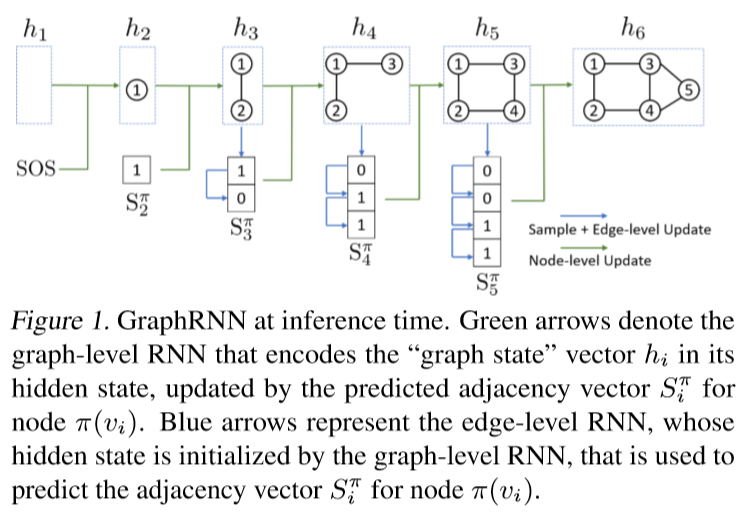
\includegraphics[width=.8\textwidth]{pics/GrpahRNN.png}
    \caption{GraphRNN生成图的过程}
    %\label{fig:my_label}
\end{figure}

GraphRNN模型是基于RNN的模型,以RNN为基础,从一个起始状态,利用RNN逐步生成图的状态,每一步向图中添加一个结点,再利用RNN生成新结点与已存在结点的连接关系,接着再向图中添加结点,重复下去直至EOS。结合之前的定义,$h_i$就是在生成过程中图的状态,它是对已经生成的图的一个encode之后的结果,每步输出$h_i$后就会将$h_i$作为另一个RNN的输入---用于生成边的连接关系的RNN。以上过程就是论文中提到的两个RNN---gaph-level RNN, edge-level RNN。
结合生成图的算法,我们可以知道有这几个部分是比较关键的:$f_{trans}, f_{out}, \mathcal{P}_{\theta_i}$。论文中对这部分都是采用神经网络来实现的,在我理解中$f_{tarns}$就是graph-level 的RNN,被$\theta_i$参数化的$\mathcal{P}_{\theta_i}$({\color{red}论文中没有对其进行详细的说明,$\mathcal{P}_{\theta_i}$具体是什么形式的呢?是全局共用一个$\mathcal{P}_{\theta_i}$吗?})用于生成边的连接关系,即一个二进制序列。
有一个值得注意的点:$S^{\pi}_i$是一个不定长的序列,但是RNN的输入是定长的。论文中是这样处理的这个问题的:采用BFS遍历图,可以得到每个结点的依赖关系,通过对图数据集进行分析,可以得到每个节点依赖的已生成结点的数量$M$的分布,最终在训练时固定下M,即在训练时每个结点所依赖的结点数是确定的,$M$是个超参数。

\par 那么如何进行训练呢?(这部分论文中并没有进行详细的描述,代码中有较详细的过程)\\
首先要将传统格式的图数据转换为论文中定义的序列形式的图。对于每个图,会对其结点进行多次排列,得到多次结点的不同序列,然后根据BFS算法对其进行遍历,可以得到在不同排列下的图生成序列。这样一个图的概率$p(G)$就可以通过求联合分布的边缘分布得到了。其次,在训练的过程中,使用了Teacher Forcing的技术进行训练。


\par 看看这篇论文是否解决了一开始所提到的几个难点呢?
\begin{itemize}
    \item 生成空间太大且可变。个人理解论文中的graph-level和edge-level 的RNN相当于对图进行了编码,能否看作是对整个图的嵌入呢?
    \item 使用序列来表示图的生成过程,将一个确定的图的概率表示为联合概率$p(G, S^{\pi})$的边缘分布。
    \item 复杂的依赖关系。使用BFS遍历图,得到数据集中每个结点所依赖的结点的数量的分布,固定下来作为超参数。(\textbf{{\color{red}这是否可以作为一个改进的点呢?}})
\end{itemize}

\par 未来工作的方向。生成更大规模的图,高效地生成指定条件的图。

其他参考资料:
\begin{enumerate}
    \item \href{https://machinelearningmastery.com/teacher-forcing-for-recurrent-neural-networks/}{What's teacher forcing fir Recurrent Neural Networks?}
\end{enumerate}


\subsection{Combining Label Propagation and Simple Models OUT-PERFORMS Graph Networks}
\begin{center}

  \begin{tabular}{rp{16cm}lp{20cm}}%{rl}

  % after \\: \hline or \cline{col1-col2} \cline{col3-col4} ...

  论文地址:& \href{https://arxiv.org/pdf/2010.13993.pdf}{https://arxiv.org/pdf/2010.13993.pdf} \\
  来源:& ICLR, 2021\\
  作者:& Qian Huangz, Horace He, et al. \\

  源码:& \href{https://github.com/CUAI/CorrectAndSmooth}{CorrectAndSmooth} \\

%  slides:& \href{http://yunshengb.com/wp-content/uploads/2017/03/nips_2018_r2l_workshop_talk.pdf}{{\footnotesize Convolutional Set Matching for Graph Similarity}}\\

  关键词:& \textbf{Label Propagation, Transductive node classification } \\

  写于:& \date{2021-03-25}

  \end{tabular}

\end{center}

该论文\cite{huang2020combining}针对GNN的解释性不足,GNN模型越来越大的问题,提出了“小米加步枪” --- 用简单模型得到和GNN一样的水平。针对trnasductive的节点分类问题,作者使用浅层模型加上LP(Label Propagation)和两个后处理方法 --- Correct \& Smooth,达到或超过了GNN在一些transductive结点分类上的效果。

\paragraph{问题定义}
给定一个图$G = (V, E)$,结点特征矩阵为$X \in \mathbb{R}^{n \times p}$,结点集$V$可以分为$U, L$分别表示无标签、有标签结点子集。标签矩阵为$Y \in \mathbb{R}^{n \times c}$。目标就是基于以上所给的信息,预测$U$中结点的标签。

\paragraph{Correct and Smooth}
论文的方法总体过程可以分为三步:
\begin{enumerate}
	\item 使用浅层模型,在$L$上,根据结点的特征做一个基础的预测,即找到$\mathop{\arg\min}\limits_{f}\: l(f(x_i), y_i)$,得到基础预测$Z \in \mathbb{R}^{n\times c}$;
	\item 利用标签数据的信息去改正基础预测$Z$;
	\item 根据相邻结点的相似性,对改正后的预测进行平滑;
\end{enumerate}

\begin{figure}[h]
	\centering
	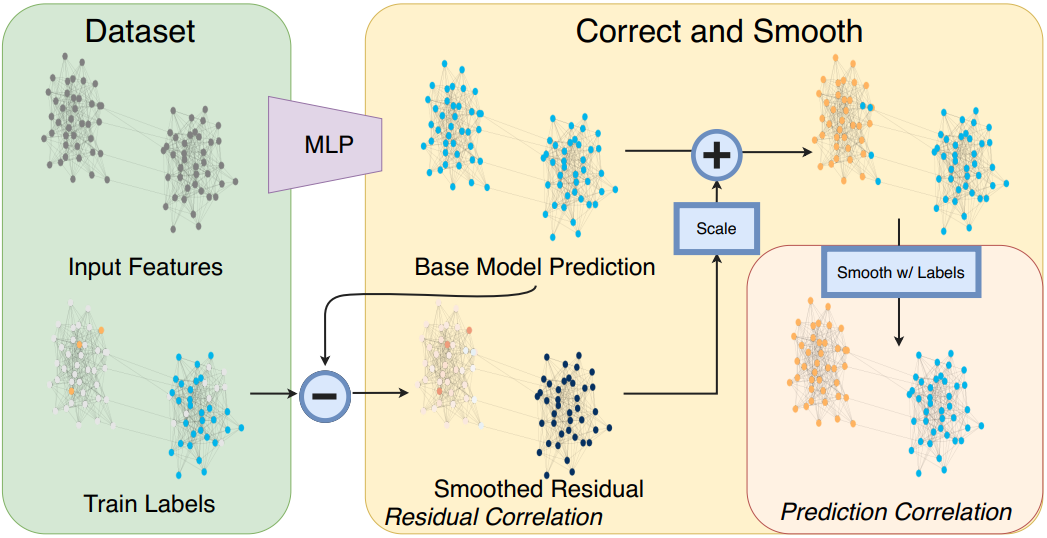
\includegraphics[width=.8\textwidth]{pics/C&S.png}
	\caption{Correct and Smooth}
	\label{fig:C&S}
\end{figure}

\subparagraph{Simple Base Predictor}
找到一个浅层模型$f$,如线性模型、MLP等,在训练数据($L$的子集)上达到最小经验损失。这一步并不会使用到图的结构,可以避免GNN模型的可扩展性问题。

\subparagraph{Correct error in base prediction with Residual Propagation}
在上一步已经有了一个基础的预测$Z$,而且有标签矩阵$Y$,可以根据二者在训练集($L_t$)上构建误差矩阵$E$,也就是residual,即:
$$
E_{L_t} = Z_{L_t} - Y_{L_t},\quad E_{L_v} = 0,\quad E_{U} = 0
$$
作者使用LP对$E$进行了平滑,平滑的公式为:
$$
\hat{E}=\underset{W \in \mathbb{R}^{n \times c}}{\arg \min } \operatorname{trace}\left(W^{T}(I-S) W\right)+\mu\|W-E\|_{F}^{2}
$$
其中$S$为$D^{-\frac{1}{2}}AD^{-\frac{1}{2}}$。上式的第一项保证$E$在$G$上的平滑,第二项保证$\hat{E}$不会偏离$E$太多。上式可以通过迭代求解,迭代式为:$E^{(t+1)} = (1-\alpha)E + \alpha SE^{(t)}$,其中$\alpha = \frac{1}{1+\mu},\: E^{(0)} = E$。得到了$\hat{E}$然后呢?当然是修正$Z$啦!$Z^{(r)} = Z + \hat{E}$。

那么问题来了,为什么要这样呢?\tbc{red}{$Z$中的误差会沿着图中的边传播,结点$i$处的误差会使得$i$的邻居产生类似的误差,应当将这种误差 --- 不确定性传播出去,即文中的error-correlation}! 

但是有一个问题:
$$
\left\|E^{(t+1)}\right\|_{2} \leq(1-\alpha)\|E\|_2 +\alpha\|S\|_{2}\left\|E^{(t)}\right\|_{2}=(1-\alpha)\|E\|_{2}+\alpha\left\|E^{(t)}\right\|_{2}
$$
因此$\left\|E^{(t)}\right\|_{2} \leq\|E\|_{2}$,可见在迭代求解过程中误差信息有一定损失,因此作者提出了对误差信息进行缩放。作者提出了两种缩放方法:
\begin{itemize}
	\item Autoscale。因为在$L_t$上的误差是知道的,因此以$L_t$上的平均误差为比例进行缩放。即$Z_{i,:}^{(r)}=Z_{i,:}+\sigma \hat{E}_{:, i} /\left\|\hat{E}_{:, i}^{T}\right\|_{1} for\:i \in U$,其中$\sigma = \frac{1}{|L_t|}\sum_{j \in L_t} ||e_j||_1$,其中$e_j$为$E$的$j-th$行;
	 
	\item Scaled Fixed Diffusion。在迭代过程中保持标签数据上的误差不变,即$E_U^{(t+1)} = [D^{-1}AE^{(t)}]_U,\: E_L^{(t)} = E_L$;
\end{itemize}

所以呢 $Z^{(r)} = Z + \text{Scale}(\hat{E})$,$\text{Scale}$ 的方式则视情况而定啦。

\subparagraph{Smoothing final prediction with Prediction Correlation}
通过上一步已经得到了$Z^{(r)}$,这一步是对$Z^{(r)}$的“平滑”。这一步的动机是:\textbf{相邻的结点相似,更可能具有相同的标签,即文中的prediction correlation},这一步再次借助LP对结点的标签分布进行平滑。

首先构造一个$G$中结点的标签分布$P \in \mathbb{R}^{n \times c}$,$P_{L_t} = Y_{L_t},\: G_{L_v, U} = Z^{(r)}_{L_v, U}$。接着就是平滑了,也是一个迭代的过程:$P^{(t+1)} = (1-\alpha)P + \alpha SP^{(t)}$,一直迭代到收敛得到最终的收敛$\hat{Y}_{ij}$。

\paragraph{总结}

\begin{itemize}

	\item 没用一股脑地上深度模型(当然,GNN大多不是深层的)。浅层模型+LP在transductive node classification上的效果直追/超过了一些GNN模型;
	\item 论文中的方法效果不错,且大大降低了模型的参数量、学习时间,速度快;
	\item 不足的是只能进行transductive的任务,目前的趋势是inductive learning;
	\item 不知道该论文的方法在其他任务上会有怎样的效果;

\end{itemize}



\subsection{Graph Structure of Neural Networks}
\begin{center}

  \begin{tabular}{rp{6cm}lp{12cm}}%{rl}

  % after \\: \hline or \cline{col1-col2} \cline{col3-col4} ...

  论文地址:& \href{https://arxiv.org/abs/2007.06559}{https://arxiv.org/abs/2007.06559} \\

  源码:& \href{https://github.com/facebookresearch/graph2nn}{graph2nn} \\

  slides:& \href{https://cs.stanford.edu/~jiaxuan/files/Graph_Structure_of_Neural_Networks_slides.pdf}{{\footnotesize Graph Sturcture of Neural Networks}}\\

  关键词:& \textbf{Neural Networks, Graph Analysis} \\

  写于:& \date{2020-10-14}

  \end{tabular}

\end{center}


这篇论文\cite{you2020graph}从图的角度来解释神经网络(Neural Networks, NN),用relational graph来对NN进行建模,并在relational graph的基础上定义了NN训练的过程。在最短路径和聚集系数的基础上分析NN的性能。以这样的视角来解释和分析NN是一个新颖的角度,\tred{为设计NN和解释NN提供了新的思路}。

\paragraph{如何建模NN为图?}引用文中的一句话:focus on message exchange, rather than just on directed data flow。建模的关键出发点是对NN中神经单元之间信息的交换,而不是信息的流向。想象如果给你一个图$\mathcal{G(V, E)}$,怎么把它看作一个NN呢,NN的训练如何在其上展开呢?论文中把$\mathcal{G}$称为relational graph。一个NN会有多层,可是一个图只有这么多结点,那么怎么训练这个“图化”后的NN呢?论文中使用round来对应NN中的层。则NN中信息在层间传递时,在$\mathcal{G}$中看起来是这样的:
$$
\boldsymbol{x}_v^{(r+1)} = AGG^{(r)} ( { f_v^{(r)} ( \boldsymbol{x}_u^{(r)}, \forall u \in N(v) ) } )
$$
其中,$\boldsymbol{x}_v^{(r)}$是结点$v$在第r round时的特征,$N(v)$是结点$v$的邻居(relational  graph中的结点都是自环的)。$AGG$类似于NN中的激活函数,$f$则类似于NN中的对上一层的输入进行线性组合或这卷积操作等。这看起来和基于消息传递的GNN模型看起来是很相似的。
\newline

论文中基于relational graph对现有的一些NN进行了分析,如固定宽度的MLP、可变宽度的MLP、ResNet的一些变体等,使用relational graph进行训练,并分析了NN“图化”后的结构与性能之间的关系。

\paragraph{方法解决的问题/优势}
\begin{itemize}
	\item 开创性的将NN视作图数据进行分析(哎,我也想到了这个点子)
	\item 以图的视角分析NN或许能够对NN的设计和理解产生很大影响
%	\item 

\end{itemize}

\paragraph{方法的局限性/未来方向}
\begin{itemize}
	\item 个人认为论文中对NN建模为relational graph的想法很不错,也很符合现在的GNN做法,但是对于复杂的NN,以及NN中的一些特殊的操作,论文中的relational graph就有点简单了,\tbc{red}{难以表现复杂的NN结构}
	\item 对relational graph的分析还比较少,局限于最短距离和聚集系数,可以分析图中的局部性的结构,如团、子图、motif等,以及一些其他的角度
	\item \tbc{red}{有期望能够打通GNN和NN之间的联系,或许在此之上能够提出新的深度学习模型!!!}
	\item 在论文基础上对NN进行解释
\end{itemize}





\subsection{Graph Convolutional Policy Network for Goal-Directed Molecular Graph Generation}
\begin{center}

  \begin{tabular}{rp{6cm}lp{12cm}}%{rl}

  % after \\: \hline or \cline{col1-col2} \cline{col3-col4} ...

  论文地址:& \href{https://arxiv.org/abs/1806.02473}{https://arxiv.org/abs/1806.02473} \\

\textbf{}  源码:& \href{https://github.com/bowenliu16/rl_graph_generation}{rl\_graph\_generation} \\

%  slides:& \href{http://yunshengb.com/wp-content/uploads/2017/03/nips_2018_r2l_workshop_talk.pdf}{{\footnotesize Convolutional Set Matching for Graph Similarity}}\\

  关键词:& \textbf{Graph Generation, Molecular Graph, Reinforcement Learning} \\

  写于:& \date{2020-10-21}

  \end{tabular}

\end{center}

该论文\cite{you2019graph}主要针对的是指定目标下的图生成问,论文的主要面向领域是药物发现,目的是生成满足某种属性以及约束条件的图。针对这个问题,论文提出了GCPN(Graph Convolutional Policy Network) --- 一种强化学习模型,通过策略梯度(policy gradient)来优化指定领域的奖励和对抗损失,在领域特定的约束环境中生成符合要求的图。

\begin{figure}[h]
	\centering
	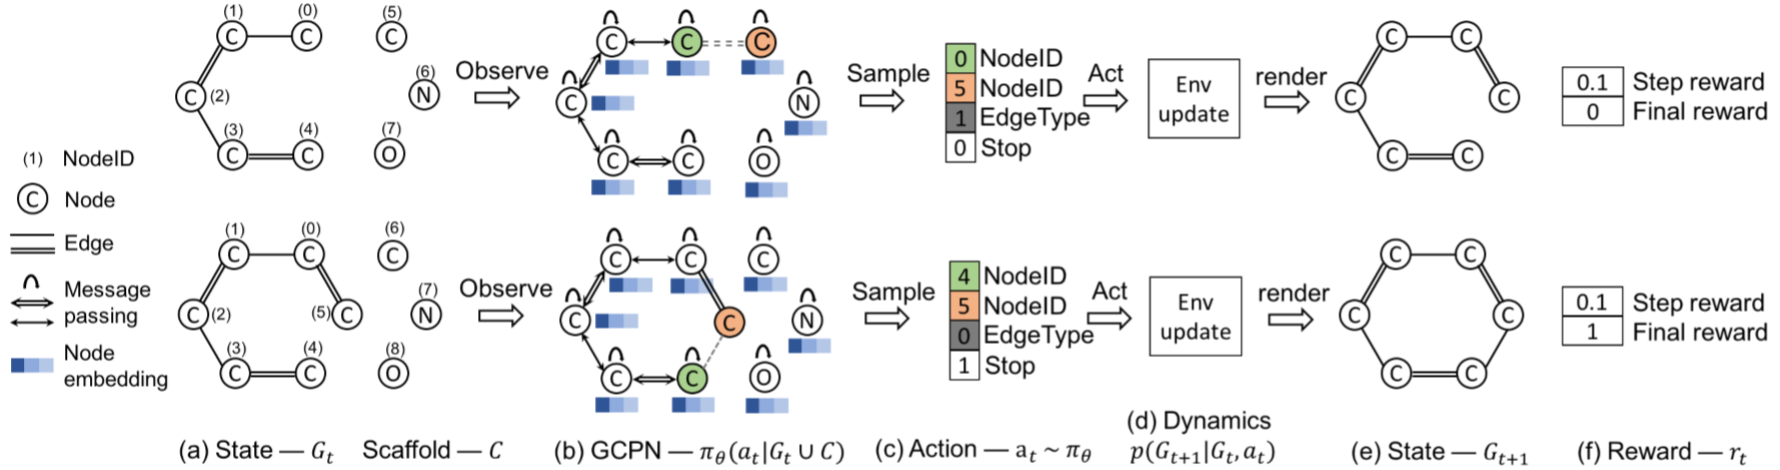
\includegraphics[width=.83\textwidth]{pics/GCPN.PNG}
	\caption{Overview of GCPN}
	\label{fig:gcpn}
\end{figure}

\paragraph{GCPN思路}整体过程如Fig.\ref{fig:gcpn}所示。在生成一个分子的过程中,是逐步通过将子结构连接到分子中或者添加边来完成的。生成一个有效分子的过程可以视作马尔可夫决策过程,从最起始的分子开始,通过执行动作进行状态转移,每个分子就是一个状态。其中,最重要的就是如何选取动作,即在每个状态下执行什么样的动作:$p(a_t | s_0,...,s_t)$,那么下一个状态就是:$p(s_{t+1} | s_0,...,s_t, a_t)$。论文中通过策略网络(policy network)来模拟$p(a_t | s_0,...,s_t)$。生成一个动作$a_t$后,会经过一些药物/化学方面的检验,来决定是否执行$a_t$,如果执行则会增加reward(即强化学习中的reward)。

需要强调的是,GCPN是通过RL来训练的,训练时不仅要考虑生成的动作是否符合要求还要考虑最后生成的分子是否满足某些性质及满足的程度。


\paragraph{方法解决的问题/优势}
\begin{itemize}
	\item 以目标导向的图生成问题来解决药物合成的问题,并且能满足药物需要满足的性质
	\item 以RL agent来对药物空间进行探索,生成的药物不一定与训练数据的分布一致,因为新的分子可能与训练数据的分布有较大差别,但是满足分子应有性质
	\item \tbc{red}{将不可微的分子的属性和一些先验条件加入到模型中}监督模型的训练,使模型向期望的方向发展

\end{itemize}



\paragraph{方法的局限性/未来方向}
\begin{itemize}
	\item 可以将模型应用到更广的范围,按照先验条件生成符合指定条件的图数据
	%\item 

\end{itemize}






\subsection{Deep Graph random Process for Relational-Thinking-based Speech Recognition}
\begin{center}

  \begin{tabular}{rp{16cm}lp{20cm}}%{rl}

  % after \\: \hline or \cline{col1-col2} \cline{col3-col4} ...

  论文地址:& \href{https://smcnus.comp.nus.edu.sg/wp-content/uploads/DGP.pdf}{https://smcnus.comp.nus.edu.sg/wp-content/uploads/DGP.pdf} \\

  %源码:& \href{xxx}{xxx} \\

  slides:& \href{https://smcnus.comp.nus.edu.sg/wp-content/uploads/DGP_slides.pdf}{{\footnotesize slides}}\\

  关键词:& \textbf{ASR, Relational Thinking, Deep Graph} \\

  写于:& \date{2020-12-10}

  \end{tabular}

\end{center}

该论文\cite{dgp}针对语音领域中如何对感知(percept)建模,并将感知融入到语音相关的问题中进行了探索,提出了一个贝叶斯非参数化的深度学习方法(Bayesian nonparametric deep learning method)--- Deep Graph random process(DGP),使用Graph对感知进行建模。

\paragraph{问题定义}
Relational Thinking是人类学习过程中至关重要的一个过程,在学习的过程中,我们会接收到各种各样的信息,不管是来自视觉、听觉、触觉等,但是我们并不会有意识地去保存它们(这是与Relational Reasoning的主要区别,relational reasoning是有意识地处理这些relation information)。在各种各样的信息之间隐藏着联系,这些信息及它们之间的联系组成了我们的percepts(感知)。论文针对语音/对话中信息之间隐藏的relation进行研究。

在通常的ASR(Automatic Speech Recognition)任务中,整个任务被分为两个过程:语音建模、语言解码,即以模式匹配的方法来解决这个问题。这种方法有一个很明显的缺点:没有考虑relational information,当然,如何将relational thinking融入到ASR中是很困难的。\tbc{red}{在交谈过程中,我们形成的感知是无意识的、无穷的}。有一些研究已经表明,在问答系统中,即使只将前一段对话的内容考虑到语音模型中,也会大大地提高模型的效果。但\tbc{red}{对percepts进行建模是很困难的} --- 这也是论文重点解决的问题。

目前,混合的语音循环神经网络隐马尔可夫模型(RNN-HMM)在许多方面仍优于端到端的编码-解码的方法,而且也越来越流行。RNN确实能够捕捉时间上的依赖关系,但对于复杂的关系(如relational thinking)则表现得不足。Graph能够描述更复杂的关系。但是依然存在一些挑战:
\begin{itemize}
	\item Graph相关的方法通常要求输入的数据是Graph形式的数据。但是在语音中并没有直接的图数据
	\item 目的是对relational thinking进行建模。但是在语音中percepts是隐含的
\end{itemize}


\paragraph{DGP 思路}DGP将relational thinking中的percepts建模为概率图,并且不需要任何关系数据。接下来更具体地描述DGP是如何对percepts进行建模的。

在语音中,处理的基本单位可以是音频数据的一个采样点、语音帧、语音片段(utterance)、一段语音等。论文中考虑的utterance,一个utterance可以是一句话的发音。在DGP中,给定一个utterance以及它之前的utterances(即历史utterances),可以生成无数个percept graphs,这与之前说到的relational thinking是相对应的。当前utterance和历史utterances之间不同的连接关可以看作一个percept(也许这就是它们称作\tbc{red}{percept graphs}的原因吧。以utterances连接成的Graph来定义percept)。为什么是无数个percept grpah呢?可以从直觉上来理解,在我们接收信息时,信息之间并没有生成稳定的信息,各个信息之间都是会产生关联的,并且基于我们的先验知识和历史信息,会在脑海中产生各种各样的理解 --- 相当于接收到的信息的不同组合,而这个组合是有无限可能的。并且,由于这些percepts是无意识的,percept graph中边的概率是接近于0的。

在DGP的percept graph中,Graph中的结点表示utterance,边表示结点之间的关系。论文中假设边的取值都服从Bernuli分布,且边的取值(即边存在的概率)是趋近于0的。看到这里貌似解决了对percepts建模的问题,但是该怎么解决涉及无数个percept graphs的问题呢?论文中对无数个percept graphs进行了transform,在percept graphs的基础上生成\tbc{red}{summary graph}。获得summary graph后即可将graph embedding作为语音模型的额外输入来提高模型性能。那么如何操作呢?

\paragraph{实现细节}
先定义一些形式化的表示。$U_i$表示utterance $i$,$U_{i-o:i-1}$表示$U_i$之前的$o$个utterances。$U_i$的特征是一系列的语音特征$\boldsymbol{X}_i = \{\boldsymbol{x}_{i,1}, \boldsymbol{x}_{i,2}, ... ,\boldsymbol{x}_{i,T}\}$,对应的标签为$\boldsymbol{Y}_i = \{\boldsymbol{y}_{i,1}, \boldsymbol{y}_{i,2}, ... , \boldsymbol{y}_{i,T}\}$。$\{ \alpha_{i,j}^{(k)} \}_{k=1}^{+\infty}$表示第$k$个percept graph中$U_i, U_j$间边存在的概率。$\{U_i\}_{i=1}^{M}$是用于训练模型的$M$个utterances。
\subparagraph{Deep Graph Random Process}
Deep Graph Random Process是一个随机过程,描述了一个机制,该机制主导无穷个概率图生成 --- 即无穷个percept graphs的生成。在percept graph中,每个结点是utterance的embedding:
$$
\boldsymbol{v}_i = f_{\theta}(\boldsymbol{X}_i)
$$
其中$f_{\theta}$是NN(Neural Network)。
DGP的核心是一系列的深度Bernuli过程(DBP),每一个DBP负责一对结点间边的生成,即:
$$
\{ \alpha_{i,j}^{(k)} \}_{k=1}^{+\infty} \sim DBP(Bern(\lambda_{i,j}))
$$
其中$Bern(\lambda_{i,j})$表示结点$i,j$间服从概率为$\lambda_{i,j}$的Bernuli分布,所有的percept graphs的边的概率都是从对应的Bernuli分布中采样的!

\subparagraph{Coupling of Innumerable Percept Graphs}
这一步的目的是如何生成summary graph,因为summary graph本身也是probablistic graph,而且结点已知,那么只剩节点之间边的概率了。其实从上一步就可以看出,单个percepet graph中边是服从Bernuli分布的,单考虑一条边的话,summary graph中对应边就是重复的Bernuli抽样,所以可以把summary graph中的边看作是服从Binomial分布的。那么summary graph中边的概率为:
$$
\tilde{ \alpha}_{i,j} = \sum_{k=1}^{+\infty} \alpha_{i,j}^{(k)},\;\; \tilde{ \alpha}_{i,j} \sim \mathcal{B}(n, \lambda_{i,j})
$$
但上式存在一个问题,$n \rightarrow +\infty,\; \lambda_{i,j} \rightarrow 0$,那么该如何解决这个问题呢?

\subparagraph{Inference and Sampling of Edges of Summary Graph}
为了采样得到summary graph中边的概率,论文中采用一个高斯分布来近似上文提到的Binomial分布。对于每条边,近似的高斯分布为:
$$
\mathcal{N}(m_{i,j}, m_{i,j}(1-m_{i,j})),\;\; m_{i,j} = n\lambda_{i,j}
$$

\subparagraph{Application of DGP for Acoustic Modelling}
为了从summary graph中提取出更具有代表性的信息,或者说为了更好地适应下游的任务,还需要对summary graph进行一个转换。转换的方式是赋予每条边一个权重,生成新的图 --- \textit{task-specific graph}(\tbc{red}{这样做的原理论文中并没有给出})。这很像注意力机制。权重是从一个高斯分布中采样得到的,那么task-specific graph的边表示为:
$$
\overline{ \alpha}_{i,j} = s_{i,j} * \tilde{ \alpha}_{i,j}
$$
上式中$s_{i,j}$是对应边的权重,论文中对权重服从的高斯分布进行了一定的假设:权重是以summary graph边的取值为条件的,即:
$$
s_{i,j}|\tilde{ \alpha}_{i,j} \sim \mathcal{N}(\tilde{ \alpha}_{i,j} * \mu_{i,j}, \tilde{ \alpha}_{i,j} * \sigma_{i,j}^2)
$$
得到task-specific graph后,即可按照GNN/GCN的方式获得graph embedding(注意:每处理一个utterance时都会有对应的task-specific graph)。接下来就是应用上述一系列工作的结果 --- graph embedding了。论文中将整个框架称作 relational thinking network(RTN),使用simple recurrent unit(SRU)作为构建单元。具体的可以参考SRU,说明一下如何在acoustic model中使用graph embedding:将graph embedding与原来的输入进行拼接即可。

\subparagraph{Learning}
知道了上述步骤,那么如何来学习整个模型呢?论文中使用variational inference来联合训练DGP、task-specific graph中边的权重、acoustic model。这个可以参考\cite{kingma2014autoencoding},目标函数是evidence lower bound(ELBO):
\begin{equation}\nonumber
	\begin{array}{l}
		\sum_{i=1}^{M}\left\{\mathrm{KL}\left(q\left(\tilde{\mathbf{A}}, \mathbf{S} \mid \mathbf{X}_{i-o: i}\right) \| p\left(\tilde{\mathbf{A}}, \mathbf{S} \mid \mathbf{X}_{i-o: i}\right)\right)\right. \\
		\left.\quad-\mathbb{E}_{\tilde{\mathbf{A}}, \mathbf{S}}\left[\log P\left(\mathbf{Y}_{i} \mid \mathbf{X}_{i}, \tilde{\mathbf{A}}, \mathbf{S}\right)\right]\right\}
	\end{array}
\end{equation}
其中,$\tilde{\mathbf{A}} = [\tilde{ \alpha}_{i,j}],\;\; \mathbf{S} = [s_{i,j}]$。上式可以转化为:
\begin{equation}\nonumber
	\begin{aligned}
		\sum_{(i, j) \in \tilde{E}}\{& \mathrm{KL}\left(\mathcal{B}\left(n, \tilde{\lambda}_{i, j}\right) \| \mathcal{B}\left(n, \tilde{\lambda}_{i, j}^{(0)}\right)\right.\\
		&+\mathbb{E}_{\tilde{\alpha}_{i, j}}\left[\mathrm{KL}\left(\mathcal{N}\left(\tilde{\alpha}_{i, j} \odot \mu_{i, j}, \tilde{\alpha}_{i, j} \odot \sigma_{i, j}^{2}\right)\right.\right.\\
		&\left.\left.\| \mathcal{N}\left(\tilde{\alpha}_{i, j} \odot \mu_{i, j}^{(0)}, \tilde{\alpha}_{i, j} \odot \sigma_{i, j}^{(0)^{2}}\right)\right]\right\}
	\end{aligned}
\end{equation}
但并不能直接最大化上式来作为优化目标,因为其中会涉及到$n \rightarrow +\infty$,所以还需要对其进行转化,具体的转化过程可以参考论文中的证明和附带材料。

Okay,整个过程就是这样了,整体框架如Fig.\ref{fig:dgp}所示。论文中还对RTN的具体实现进行了介绍,包括上文中涉及到的一些参数的计算,如$m_{i,j}, \mu_{i, j}, \sigma_{i, j}$等,以及模型的网络结构等。
\begin{figure}[h]
	\centering
	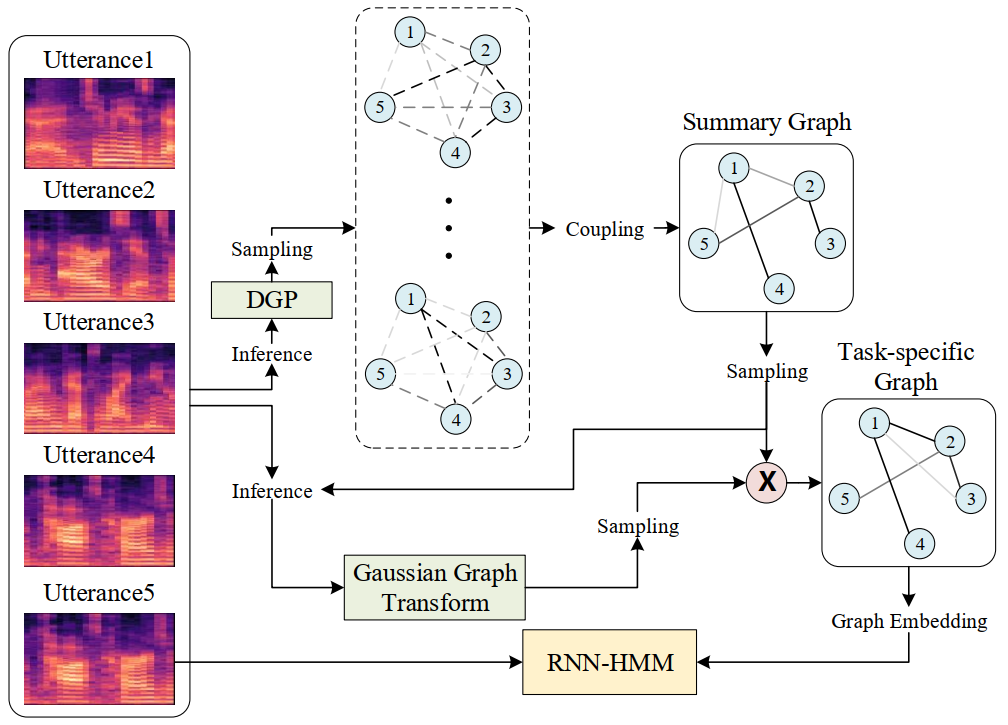
\includegraphics[width=.8\textwidth]{pics/dgp.PNG}
	\caption{Architecture of RTN for acoustic modelling}
	\label{fig:dgp}
\end{figure}

\paragraph{方法解决的问题/优势}

\begin{itemize}
	\item 提出了一种对percept建模的方法,percept graphs的想法很棒
	\item 以graph的形式表示percepts,并无需relation data就可以学习到隐含的relational thinking
	\item 将relational thinking融入到acoustic model中
\end{itemize}



\paragraph{方法的局限性/未来方向}
\begin{itemize}
	\item 个人认为variational inference会涉及到较多的运算
	\item \tbc{red}{可以将percept graphs的想法应用到更多的问题上}
	\item task-specific graph的由来没有解释清楚	
	\item \tbc{red}{论文中只结合了历史的utterances,并没有结合先验知识}。尽管不同的人先验知识是不同的,但是在某个特定的应用场景下,先验知识是有范围的,可以借助知识图谱来表示先验知识,再结合本文的方法完成特定场景下的对话任务。\tbc{red}{这也可以看作是一个多模态信息融合的方法}
	\item 在生成summary graph时,相当于给所有的percept graphs分配了相等的权重(注意力),然而在实际的思考过程中,\tbc{red}{不同的percepts应该有不同权重的,在生成summary graph时对不同的percept graphs赋予不同的注意力是否更合理?
	}

\end{itemize}


\subsection{Learning to Represent Image and Text with Denotation Graph}
\begin{center}
	\begin{tabular}{rp{6cm}lp{10cm}}%{rl}
		% after \\: \hline or \cline{col1-col2} \cline{col3-col4} ...
		论文地址:& \href{https://arxiv.org/abs/2010.02949}{https://arxiv.org/abs/2010.02949} \\
		源码地址:& \href{https://shalab.usc.edu/DG/}{DG} \\
		关键词:& \textbf{embedding, multimodal,  Denotation Graph} \\
		写于:& \date{2020-10-08}
	\end{tabular}
\end{center}
该论文\cite{zhang2020learning}提出了一种表征多模态(图像+文本)数据的方法。存在着大量对齐的“视觉+文本”的数据,如包含描述的图片、视频、带字幕的电影等。学习如何表示这种视觉和文本存在明显的语义联系的数据是有很大引用价值的,如通过文本搜索图片、视频,为视频/图片添加描述,通过语言查询视频/图片中的信息,可视化的问答系统等。\\
\begin{figure}[h]
	\centering
	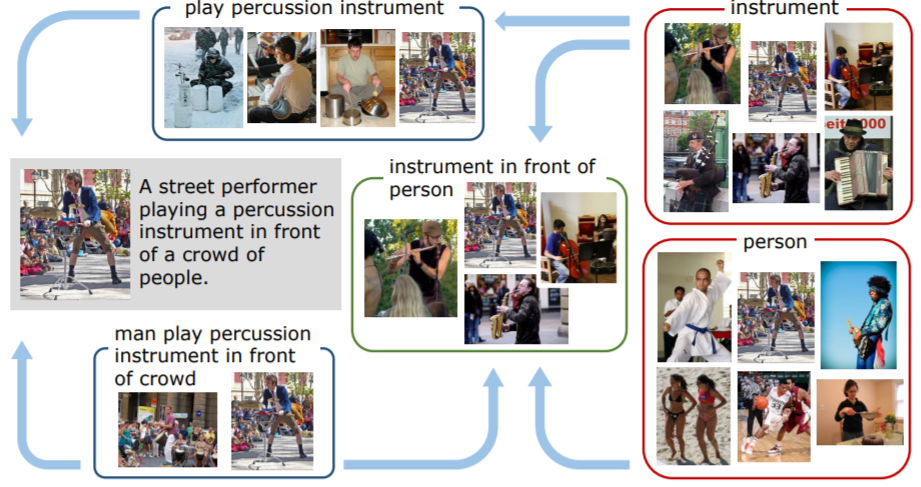
\includegraphics[width=.8\textwidth]{pics/DG.png}
	\caption{denotation graph extracted from the FLICKR30K dataset}
	\label{fig:DG}
\end{figure}
\textbf{方法}\hspace{6pt}论文中使用denotation graph(DG)\cite{young-etal-2014-image}来表示“图像+文本”的数据。该论文中的DG中每个结点包含一个文本描述和一系列与之对应的图像,图中的边是有向边,从语义上抽象的结点指向更具体地结点。如Fig.\ref{fig:DG}所示,DG中抽象的结点具有更一般的概念(如图中的person, instrument),抽象结点会指向更具体地结点(如play percussion instrument),每个结点会包含结点概念所对应的一些列图片。为什么要将文本与图像对应起来呢?论文中基于这样的一个假设:图片与文本对应的一致性有利于下游任务。在得到上述的DG(构建DG可参考\href{https://github.com/aylai/DenotationGraph}{这里}和\cite{young-etal-2014-image})后,在DG基础上学习图片和文本地表征。

\subsection{Retrieval-Augmented Generation for Code Summarization via Hybrid GNN}
\begin{center}
	\begin{tabular}{rp{16cm}lp{20cm}}%{rl}
		
		% after \\: \hline or \cline{col1-col2} \cline{col3-col4} ...
		
		论文地址:& \href{https://openreview.net/pdf?id=zv-typ1gPxA}{https://openreview.net/pdf?id=zv-typ1gPxA} \\
		来源:& ICLR, 2021 \\
		作者:& Shangqing Liu, et al. \\
		%源码:& \href{https://github.com/IBM/EvolveGCN}{EvolveGCN} \\
		
		%  slides:& \href{http://yunshengb.com/wp-content/uploads/2017/03/nips_2018_r2l_workshop_talk.pdf}{{\footnotesize Convolutional Set Matching for Graph Similarity}}\\
		
		关键词:& \textbf{GNN, Code Summarization} \\
		
		写于:& \date{2021-07-19}
		
	\end{tabular}
\end{center}
该论文\cite{liu2021retrieval-augmented}的目标:给定某种语言编写的函数代码,生成这个函数的自然语言描述。自动的代码摘要主要有两张方式:1)Retrieval-based(抽取式);2)Generation-based(生成式)。该论文提出了一种结合这两种方法的增强的抽取式方机制来进行代码总结。
\begin{figure}[h]
	\centering
	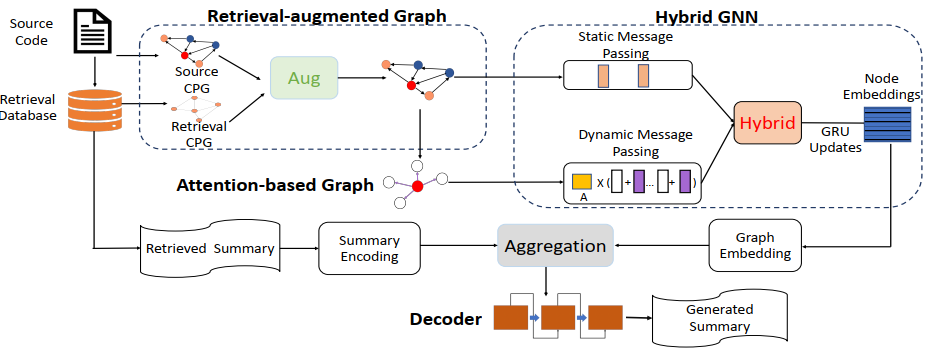
\includegraphics[width=.8\textwidth]{pics/HGNN.png}
	\label{fig:hgnn}
	\caption{Overview of HGNN}
\end{figure}

论文提出的方法是Hybrid GNN(Fig.\ref{fig:hgnn}),首先根据代码的抽象语法树表示成Graph(Fig.\ref{fig:cpg}),再从代码数据集中找到与当前代码最相似的代码(除去当前的函数)及对应的summarization,当前代码的Graph经过最相似的代码的Graph增强后得到static graph,经过注意力机制后生成dynamic graph,在static/dynamic graph上进行message passing,再通过Hybrid massage passing(即将同一个结点在static和dynamic graph中的表征融合后再进行massage passing)。除此之外,还会利用找到的最相似的代码的summarization的表征,将最终得到的结点表征与summarization表征进行拼接后输入基于注意力的LSTM,得到目标代码的表征。

\begin{figure}[h]
	\centering
	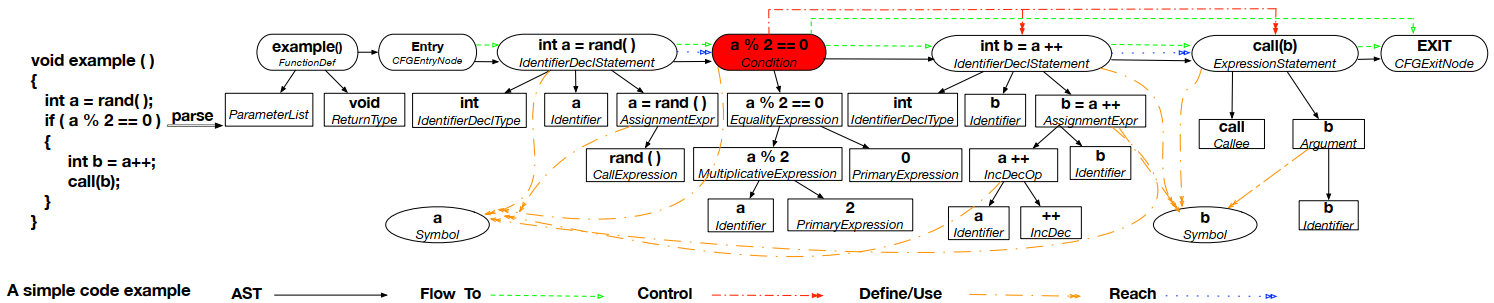
\includegraphics[width=.8\textwidth]{pics/CPG.png}
	\label{fig:cpg}
	\caption{An Example of Code Property Graph(CPG)}
\end{figure}


}{}

\ifthenelse{\boolean{gnnsim}}{
\clearpage
\section{Graph Similarity}
\subsection{graph2vec: Learning Distributed Representation of Graphs}
\begin{center}
  \begin{tabular}{rl}
  % after \\: \hline or \cline{col1-col2} \cline{col3-col4} ...
  论文地址:& \href{https://arxiv.org/abs/1707.05005}{https://arxiv.org/abs/1707.05005} \\
  源码地址:& \href{https://github.com/MLDroid/graph2vec_tf}{graph2vec} \\
  关键词:& \textbf{Graph Kernels, doc2vec, representation learning} \\
  写于:& \date{2020-09-30}
  \end{tabular}
\end{center}

论文\cite{DBLP:journals/corr/NarayananCVCLJ17}提出了图的embedding方法---graph2vec,该方法借鉴word2vec, doc2vec的思想,以rooted subgraph 作为图的元素,通过最大化似然概率来得到每个图的定长的embedding向量。

\par 如果熟悉word2vec的话,其实很容易就理解这篇论文的方法了(虽然graph2vec是在模仿doc2vec,但doc2vec开起来像在模仿word2vec)。因为graph2vec是在word2vec基础上做的,它们之间存在一个比较直白的对应关系,厘清它们之间的对应关系就明白graph2vec了。
\par 在介绍doc2vec和graph2vec的对应关系之前,先介绍一下rooted graph的概念。rooted subgraph是一个类似于树状的结构,可以看作一棵多叉树,树中的结点就是图中的结点,结点按照图中的邻接关系相连。可以根据图中的每个结点$v$生成一棵rooted subgraph,以$v$为根,它的子结点为它的邻居结点,每个子结点又以自己的邻居结点为子结点,如此递归定义下去就是以$v$为根的rooted subgraph。接下来介绍graph2vec和doc2vec之间的概念对应关系。
\par 在doc2vec中,每个doc(文档)被看做词序列的集合,优化文档向量的基础就是:最大化词序列和文档的共现率。graph2vec将一个graph看做一个文档,rooted graph看做文档中的词序列。所以优化graph embedding的基础就是:最大化rooted subgraph和graph的共现率。与word2vec类似,graph2vec中也使用了负采样的方法对算法进行优化。

\par 与最近使用GNN来进行graph embedding的方法相比,graph2vec是transductive的,对于未见过的graph需要重新运行一遍算法来生成embedding,与Deepwalk很像。我这里有一个想法,rooted subgraph能否通过其他形式来替代,比如node2vec中的游走策略生成的子图。

%\clearpage

\subsection{Convolutional Set Macthing for Graph Similarity\label{sec:GSimCNN}}
\begin{center}
  \begin{tabular}{rp{6cm}lp{12cm}}%{rl}
  % after \\: \hline or \cline{col1-col2} \cline{col3-col4} ...
  论文地址:& \href{https://arxiv.org/abs/1810.10866}{https://arxiv.org/abs/1810.10866} \\
  slides:& \href{http://yunshengb.com/wp-content/uploads/2017/03/nips_2018_r2l_workshop_talk.pdf}{{\footnotesize Convolutional Set Matching for Graph Similarity}}\\
  关键词:& \textbf{Graph Similarity, GCN, CNN} \\
  写于:& \date{2020-10-10}
  \end{tabular}
\end{center}

该论文\cite{bai2018convolutional}主要解决的问题是:给定两个图$\mathcal{G}_1, \mathcal{G}_2$,计算它们的相似性。图相似性计算是图数据搜索中的难点和核心点,由于图的同构性,衡量两个图的相似性是NP-hard问题。论文中提出了GSimCNN(Graph  Similarity Computation via Convolutional Neural Network)来解决这个问题。

\textbf{GSimCNN思路}\hspace{12pt}该方法使用了图像识别中CNN的方法,通过GCN可以得到每个graph的多个结点特征矩阵(GCN有几层就有几个节点特征矩阵),这样就得到了$\mathcal{G}_1, \mathcal{G}_2$的节点特征矩阵,再根据这两个结点特征矩阵构造一个相似矩阵(Similarity Matrix),构造方法是从$\mathcal{G}_1, \mathcal{G}_2$各取一个结点的特征矩阵做内积得到相似矩阵中的一个元素。如果GCN有k层,则可以得到k个相似矩阵。在经过CNN的一顿操作后将CNN的输出输入到一个全连接的MLp中,得到两个graph的相似度分数。损失函数是均方误差损失函数(对于$\mathcal{G}_1, \mathcal{G}_2$,会有一个实际的相似度分数)。可参考Fig.\ref{fig:GSimCNN}。

\begin{figure}[h]
	\centering
	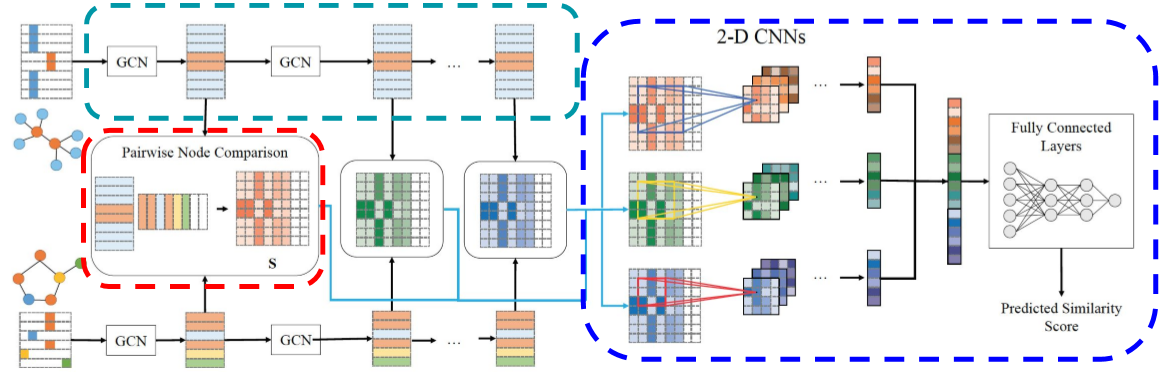
\includegraphics[width=.8\textwidth]{pics/GSimCNN.PNG}
	\caption{GSimCNN的三个阶段,分别用不同颜色的虚线框圈出}
	\label{fig:GSimCNN}
\end{figure}

如Fig.\ref{fig:GSimCNN}所示,是使用GSimCNN计算两个图相似性的过程,不同颜色代表算法的不同阶段。

{\textcolor[RGB]{64, 177, 189}{\textbf{Stage 1}}}\hspace{12pt}GCN阶段,使用一个多层的GCN为$\mathcal{G}_1, \mathcal{G}_2$中的每个结点生成表征,这样在GCN的每一层,都能够生成两个两个结点特征矩阵。若GCN有k层,则会有k对个结点特征矩阵对。{\color{red}为什么要在每一层计算一个相似矩阵呢?}因为GCN是基于汇集邻居的信息来表征的,第k层相当于汇集了k-hop的邻居的信息,而图的结构相似往往是局部的,而且是在不同尺度(图的规模)上的。而不同层的结点表征相当于代表了不同尺度的结构,也就能在不同尺度上进行图的相似性比较。  

{\color{red}\textbf{Stage 2}}\hspace{12pt}使用每一层的结点特征矩阵对,通过内积运算得到一个相似矩阵。因为GCN有k层,则会得到k个相似矩阵。

{\color{blue}\textbf{Stage 3} }\hspace{12pt}基于{\color{red}Stage 2}得到的k个相似矩阵,使用多个卷积核(Fig.\ref{fig:GSimCNN}中使用了3个2-D卷积核)来对多个相似矩阵进行卷积,最后将多个卷积核的结果向量进行拼接,输入到全连接的MLP中计算相似度分数。

在实验方面,作者使用了两类的baseline,一类是基于组合优化的近似GED(Graph  Edit Distance,相关论文表明当图地结点超过16时,GED将变得难以计算\cite{arora2019exact},因此也产生了很多近似算法)的算法,另一类的基于神经网络的算法。在这些算法中,GED的算法作为基准,其mse是0,但是复杂度太高,时间成本太高,GSimCNN与其他算法相比在mse和时间上都取得较好的效果。

论文中还有一些其他细节的处理,比如:对于不同大小的图的特征矩阵会进行padding,针对结点的排序使用了\cite{you2018graphrnn}的BFS的思路等。

至于论文的题目中的\textbf{set matching},因为沦为中使用的是Set matching的思路来计算两个图的相似性,一个图的所有结点的表征就是一个set。那为什么不适用graph-level的表征来直接计算图的相似性呢?(在论文的实验比较中有几个方法使用的就是graph-level的表征,如:EmbAvg, GCNMean, GCNMax,这几个方法在通过结点表征得到图表征时的方法不一样,如算术平均结点的表征作为图表征等)论文中给出的原因如下:
\begin{itemize}
	\item 没有使用更细粒度的结点表征
	\item 忽略了图级的交互(原文是{\color{red}{graph level interaction}},但不确定是什么意思)
\end{itemize}
也正是因为以上原因,论文将图相似性以set matching的角度来解决。个人认为论文是在更细粒度对两幅图的相似性进行了比较({{\color{red}{能否进行更细粒度的比比较呢?}}比如利用结点的属)。

论文中对GSimCNN得到的相似矩阵进行了可视化,发现相似或很不相似的图的相似矩阵都有一些明显的特点,如Fig.\ref{fig:sim}所示:
\begin{figure}[h]
	\centering
	%\hspace{1.5pt}
	\subfigure{
		\begin{minipage}{0.95\linewidth}
			\centering
			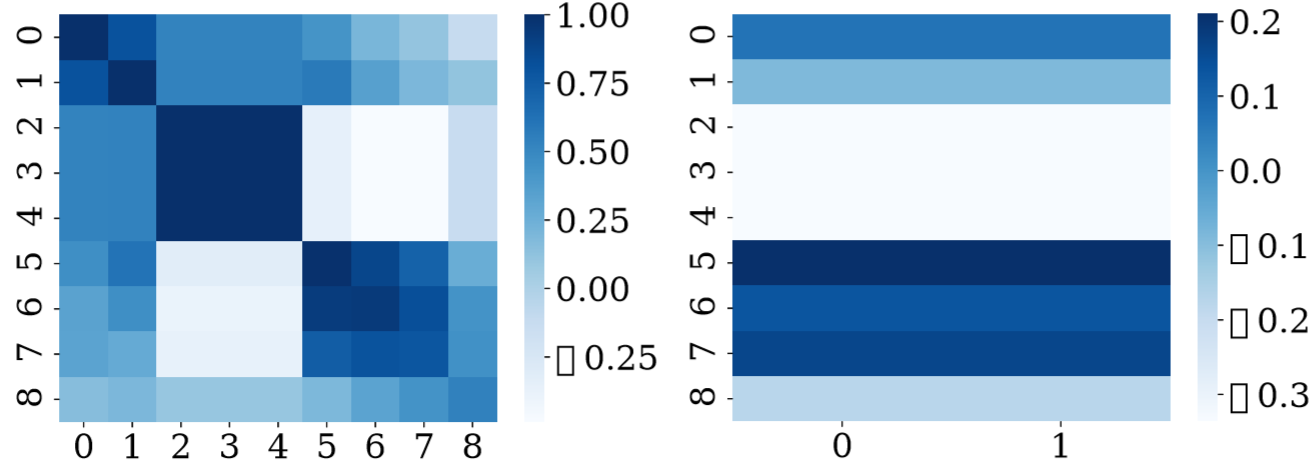
\includegraphics[width=.85\textwidth]{pics/sim1.PNG}
			\vspace{12pt}
			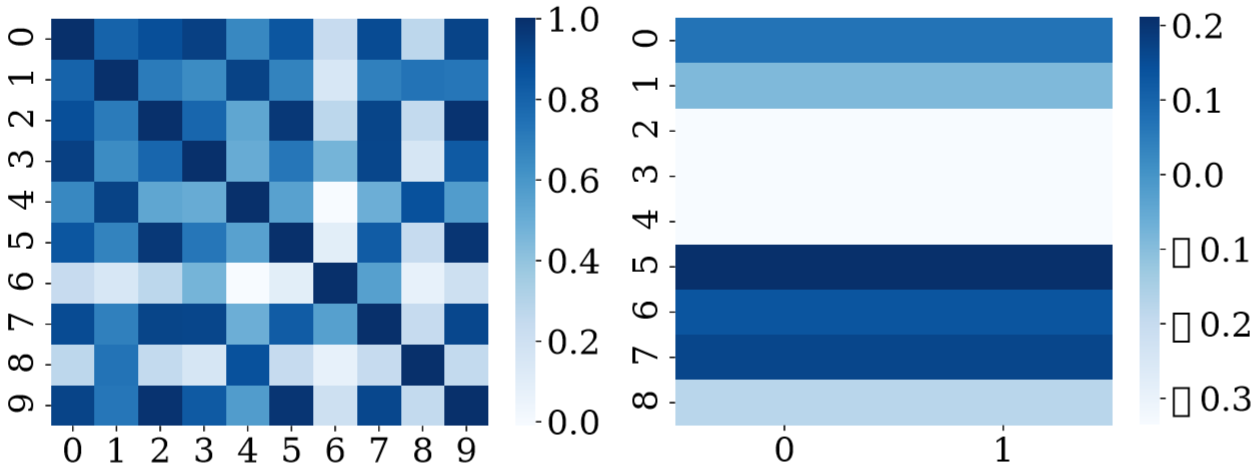
\includegraphics[width=.85\textwidth]{pics/sim2.PNG}
		\end{minipage}
	}
	\caption{左边的为相似的图的相似矩阵,右边为不相似图的相似矩阵}
	\label{fig:sim}
\end{figure}

未来工作的方向:通过生成图的编辑序列来更好地解释计算得到的相似度({\color{red}这个可以有!});使用其他的结点表征网络,如GraphSAGE;使用其他的图相似度度量方法({\color{red}比如?});在其他领域地数据上的泛化。

本篇论文的作者Yunsheng Bai在Garph Matching和Graph Similarity方面做了较多的工作,可参考\href{http://yunshengb.com/}{他的主页}。


%\clearpage



\subsection{SimGNN: A Neural Network Approach to Fast Graph Similarity Computation\label{sec:SimCNN}}
\begin{center}
  \begin{tabular}{rp{6cm}lp{12cm}}%{rl}
  % after \\: \hline or \cline{col1-col2} \cline{col3-col4} ...
  论文地址:& \href{https://arxiv.org/abs/1808.05689v4}{https://arxiv.org/abs/1808.05689v4} \\
  源码:& \href{https://github.com/yunshengb/SimGNN}{SimGNN} \\
%  slides:& \href{http://yunshengb.com/wp-content/uploads/2017/03/nips_2018_r2l_workshop_talk.pdf}{{\footnotesize Convolutional Set Matching for Graph Similarity}}\\
  关键词:& \textbf{Graph Similarity, GCN, Graph Edit Distance} \\
  写于:& \date{2020-10-13}
  \end{tabular}
\end{center}

该论文\cite{bai2019simgnn}与\ref{sec:GSimCNN}的作者相同,也是为了解决图相似性计算的问题,该论文的方法/模型与\ref{sec:GSimCNN}中的方法/模型类似。论文中提出了SimGNN(Graph  Similarity Computation via Graph Neural Network)来解决这个问题。

\textbf{SimGNN思路}\hspace{12pt}该方法针对图相似性的计算提出了两个策略(strategy),能够分别计算$\mathcal{G}_1, \mathcal{G}_2$的相似性,论文中将这俩策略结合起来一起使用。Strategy 1是通过GCN得到graph-level的图表征,基于图表征计算相似度。Strategy 2是利用图中的结点表征进行相似度的计算。Strategy 1/2 的过程可参考Fig.\ref{fig:SimGNN},细节如下。

\begin{figure}[h]
	\centering
	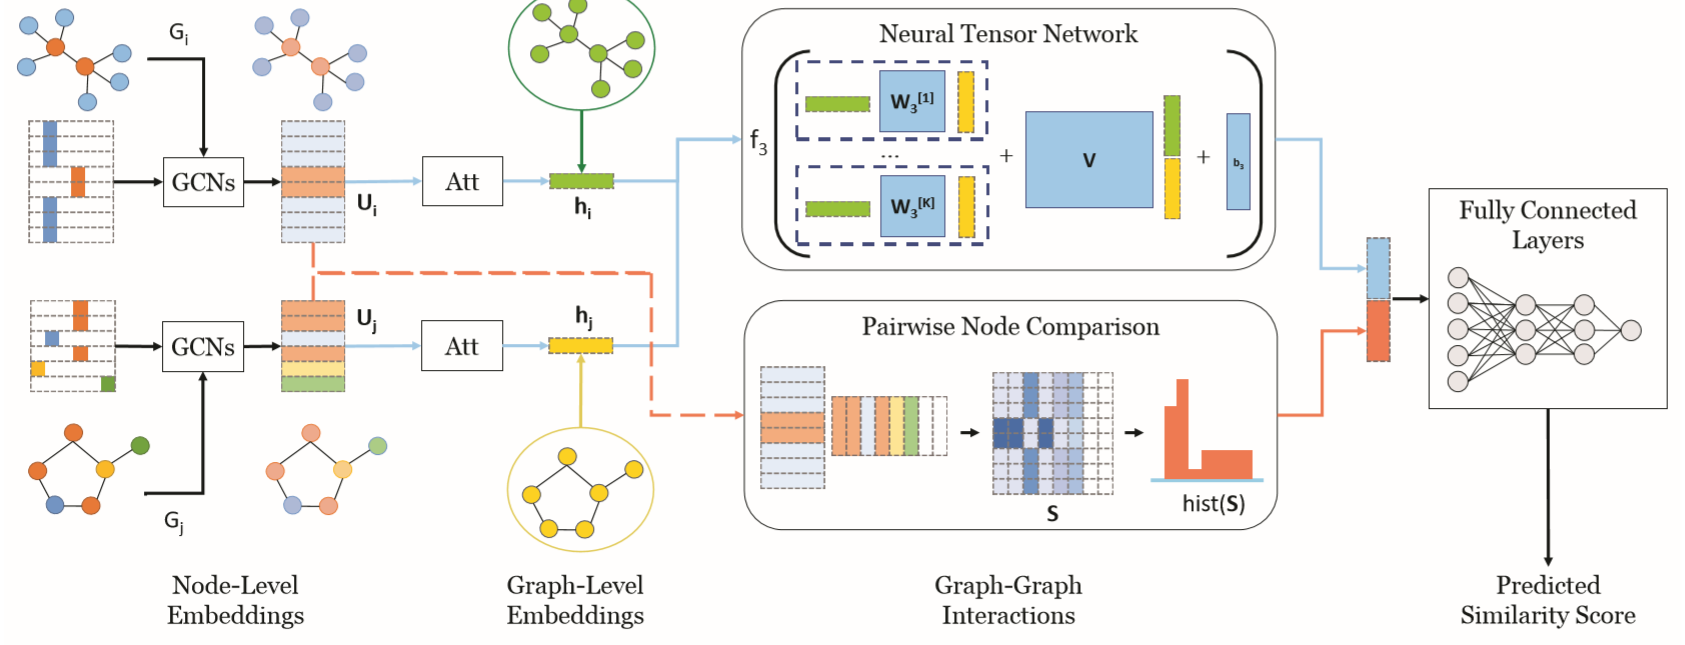
\includegraphics[width=0.8\textwidth]{pics/SimGNN.PNG}
	\caption{SimGNN}
	\label{fig:SimGNN}
\end{figure}

\paragraph{Strategy 1}Strategy 1是通过GCN计算每个结点的表征,再通过注意力的方法计算得到图的表征,该过程又可以分为4个阶段。

\subparagraph{Stage 1}计算节点表征。如Fig.\ref{fig:SimGNN}所示,通过GCN(论文中使用的\href{https://github.com/mdeff/cnn_graph}{GCN})计算得到每个结点的表征。

\subparagraph{Stage 2}计算图表征。SimGNN是以结点表征为基础,基于注意力计算图表征的。在计算图表征之前,先计算图的上下文(global  graph context)--- 上下文向量$\boldsymbol{c} = tanh(\frac{1}{N} \boldsymbol{W_2} \sum_{n=}^N \boldsymbol{u_n})$,其中$\boldsymbol{W_2}$是待学习得参数。对于任意一个结点$\boldsymbol{u_n}$,它的注意力(权重)计算方式是:$attention(\boldsymbol{u_n}) = \sigma( \boldsymbol{u_n}^\mathrm{T} \boldsymbol{c} )$。最终图$\mathcal{G}$的表征$\boldsymbol{h} = \sum_{n=1}^{N} attention(\boldsymbol{u_n}) \boldsymbol{u_n}$。

论文中特别提到了一个点 --- 没有对$attention(\boldsymbol{u_n})$进行归一化,即虽然$attention(\boldsymbol{u_n}), \forall n \in \{1, ... , N\}$是在0到1之间的,但是没有经过一个类似softmax的归一化。这是为什么呢?难道总的权重不应该为1吗?论文中给出的解释是:让最后得到的图表征反映图的大小,这对相似性计算是很重要的。很巧妙,{\color{red}并不是所有的情况都需要归一化}!
 
\subparagraph{Stage 3}使用图表征计算 Graph-Graph interaction。这里的图交互(个人翻译),指的是通过图表征计算一个相似度向量。具体操作:使用Neural Tensor Network(NTN)来对图表征之间的关系进行建模。则两个图表征之间的关系表示为$g(\boldsymbol{h_i}, \boldsymbol{h_j}) = f( \boldsymbol{h_i}^\mathrm{T} \boldsymbol{W_3^{[1:K] } } \boldsymbol{h_j} + \boldsymbol{V} \begin{bmatrix}
	\boldsymbol{h_i} \\ \boldsymbol{h_j}
\end{bmatrix} + \boldsymbol{b_3} )$。其中$\boldsymbol{W_3^{[1:K] } }$是一个张量,包括$\boldsymbol{V}和\boldsymbol{b_3}$都是待学习的参数,K是超参数,最后$g(\boldsymbol{h_i}, \boldsymbol{h_j})$的结果就是一个$\mathbb{R}^K$中的相似度向量。

\subparagraph{Stage 4}计算图相似度。从stage 3 得到两幅图的相似度向量后使用全连接的MLP计算相似度。
\newline

以上4个阶段就是Strategy 1 的全过程,使用图标表征的interacting能够反映相似度基于这样一个假设:好的图表征应该能够编码图的结构和特征信息,可以通过图表征的interacting来预测图之间的相似性({\color{red}为什么通过interacting就能反映图之间的相似性呢?})。

\paragraph{Strategy 2}使用GCN输出的结点表征,计算一个与\ref{sec:GSimCNN}中类似的相似矩阵,可以得到一个更细粒度(fine-grained)的相似评估。因为图的结点没有一个特定的排列,Strategy 2使用了一种结点排列无关的方法 --- 提取相似矩阵的直方图特征,来利用相似矩阵计算相似度。直方图的bin的数量是超参数。

将Strategy 1 和 Strategy 2结合起来使用时将Strategy 1中stage 3得到的相似度向量与Strategy 2得到的直方图特征(也是一个向量)拼接后输入到全连接的MLP中计算得到一个相似度。
\newline

至此,SimGNN的过程就说完了。总的来说,Strategy 1是从粗粒度上来计算图之间的相似性,而Strategy 2则是从更细粒度上计算结点相似性,Strategy 2能够对Strategy 1进行补充、增强(但论文中的实验说明,使用Strategy 2后并没有较大的提升)。

\paragraph{方法解决的问题/优势}
\begin{itemize}
	\item SimGNN计算相似性是结点排列无关的。也就是说,同一个图,不同的结点排列,不会影响它和其他图的相似性的计算。这主要是因为使用了相似矩阵的直方图特征
	\item 模型是inductive的,能够泛化到未见过的图。SimGNN中使用的GCN是inductive的
	\item SimGNN是end-to-end的模型,参数都是可学习的
\end{itemize}

\paragraph{方法的局限性/未来方向}
\begin{itemize}
	\item 在Strategy 2中使用直方图特征虽然是结点排列无关的,但个人认为不能充分地利用相似矩阵,这也可能是为什么Strategy 2效果不明显地原因。或许有更好的结点排列无关的方法来利用结点表征(并不一定要使用相似矩阵)
	\item 图上下文向量$\boldsymbol{c}$的原因,为什么使用它?
	\item SimGNN只使用了结点的特征,并没有{\color{red}使用边的特征},后期可以将边的特征纳入模型考虑的范畴。在一些领域,如化学领域,边的类型是很重要的
	\item 目前的图的相似性计算主要针对较小的图,如何计算大规模的图的相似性呢
	\item {\color{red}如何计算更复杂的图的相似性呢,如动态图}
\end{itemize}

作者其他工作可参考\href{http://yunshengb.com/}{他的主页}。


%\clearpage

\subsection{Unsupervised Inductive Graph-level Representation Learning via Grpah-Graph proximity}
\begin{center}
  \begin{tabular}{rp{6cm}lp{16cm}}%{rl}
  % after \\: \hline or \cline{col1-col2} \cline{col3-col4} ...
  论文地址:& \href{https://arxiv.org/abs/1904.01098}{https://arxiv.org/abs/1904.01098} \\
  源码:& \href{https://github.com/yunshengb/UGraphEmb}{UGraphEmb} \\
%  slides:& \href{http://yunshengb.com/wp-content/uploads/2017/03/nips_2018_r2l_workshop_talk.pdf}{{\footnotesize Convolutional Set Matching for Graph Similarity}}\\
  关键词:& \textbf{Graph Embedding, Unsupervised Learning} \\
  写于:& \date{2020-10-14}
  \end{tabular}
\end{center}

该论文\cite{bai2019unsupervised}与\ref{sec:GSimCNN},\ref{sec:SimCNN}的作者相同,这篇论文的目的是为了学习到图的表征,并让学习到的表征尽量保持图之间的相近关系(proximity)。学习到的表征可以作为下游任务的输入,个人认为这相当于一种与训练。论文提出了一个无监督的模型 --- UGraphEmb(Unsupervised Graph-level Embedding)基于图之间的proximity来学习图表征,并提出了多尺度(类似于\cite{bai2018convolutional}中的多尺度)的结点注意力MSNA(Multi-Scale Node Attention)。

\begin{figure}[h]
	\centering
	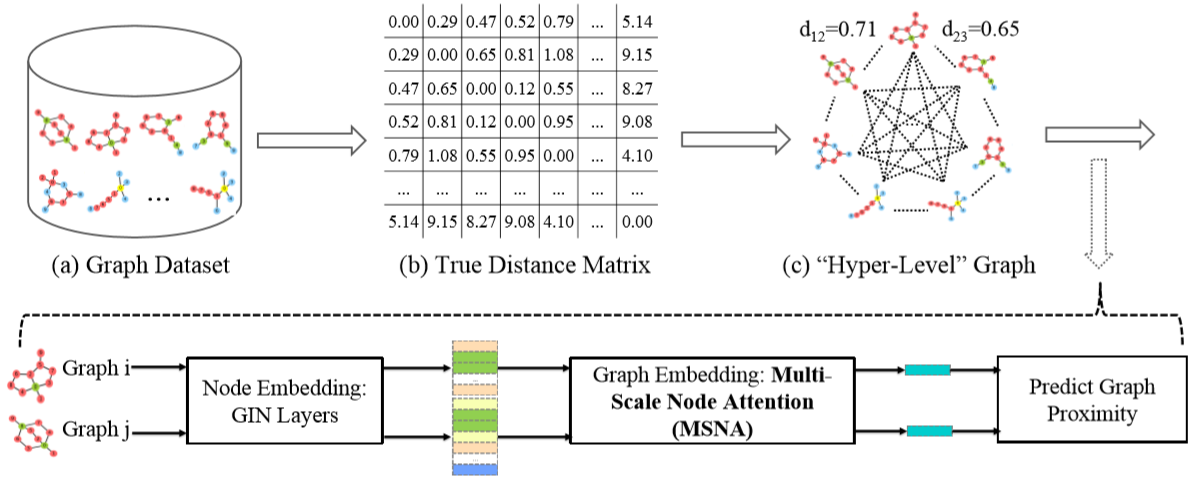
\includegraphics[width=.7\textwidth]{pics/UGraphEmb}
	\caption{Overview of UGraphEmb}
	\label{fig:UGraphEmb}
\end{figure}
% 接下来,构建一个Hyper-level graph --- 以图为结点,proximity作为边的权重。
\paragraph{UGraphEmb思路}首先,这个模型是在一个图数据集上学习的,需要先计算图数据集中两两图之间的proximity(一开始我认为是similarity,但并不是很准确,论文中使用的是GED来计算的proximity),这样就可以得到一个distance matrix,表示任意两个图之间的proximity。那么如何生成图的表征呢?使用GIN\cite{xu2018how}来学习结点表征,多尺度则体现在:以GIN的每一层生成一个图表征,再拼接在一起形成最终的图表征。其中每一层会有一个注意力,也就是MSNA。得到任意两个图的表征后,就要使用proximity了,希望模型学习到的图表征尽量保留图之间的proximity。损失函数定义如下:
% 公式换行!!!
% 其中 & 表示对齐的位置, \\ 表示换行
\begin{equation}\nonumber
	\begin{aligned}
		\mathcal{L} &= \mathbb{E}_{(i, j) \sim \mathcal{D}} (\hat{d_{ij} } - d_{ij} )\\
		&= \mathbb{E}_{(i, j) \sim \mathcal{D}} (||\boldsymbol{h_i} - \boldsymbol{h_j} ||_2^2 - d_{ij} )
	\end{aligned}
\end{equation}
其中$\hat{d_{ij} }$是关于两个图表征的proximity计算,$d_{ij}$是预先计算好的proximity。

论文中提到了\tbred{图表征的无监督学习方法的一个挑战}:与结点表征学习的不同,结点之间存在联系,可以在此基础上进行无监督学习,而图之间是没有天然的联系的(如距离/相似性)。而proximity就充当了一个这样的\textbf{Inter-Graph information},将不同的图联系起来。

\paragraph{方法解决的问题/优势}
\begin{itemize}
	\item 无监督的、inductive的图表征方法
	\item 可以作为图数据的预训练模型,下游任务在其基础上进行微调即可,如图分类、图相似性计算
\end{itemize}

\paragraph{方法的局限性/未来方向}
\begin{itemize}
	\item 能否直接在Hyper-level graph上学习图的表征与多尺度的表征融合呢?
%	\item 
\end{itemize}



%\clearpage

\subsection{Grapg-Graph Similarity Network}
\begin{center}

  \begin{tabular}{rp{6cm}lp{12cm}}%{rl}

  % after \\: \hline or \cline{col1-col2} \cline{col3-col4} ...

  论文地址:& \href{https://openreview.net/pdf?id=R3a2G2tSf3c}{https://openreview.net/pdf?id=R3a2G2tSf3c} \\

  %源码:& \href{xxx}{xxx} \\

%  slides:& \href{http://yunshengb.com/wp-content/uploads/2017/03/nips_2018_r2l_workshop_talk.pdf}{{\footnotesize Convolutional Set Matching for Graph Similarity}}\\

  关键词:& \textbf{Graph Similarity, Graph Classification, Metric Learning} \\

  写于:& \date{2020-10-15}

  \end{tabular}

\end{center}

该论文针对图分类问题提出了新的解决方案 --- Graph-Graph(G2G)。现有的图分类方法中,通常会忽略图数据之间的关系 --- 当然图数据之间也没有直观的联系。论文中以图为结点,图之间的相似性为边的权重构建了 SuperGraph,之后图的分类问题则转变成SuperGraph中结点分类的问题。G2G方法过程如Fig.\ref{fig:G2G}所示。

\begin{figure}[h]
	\centering
	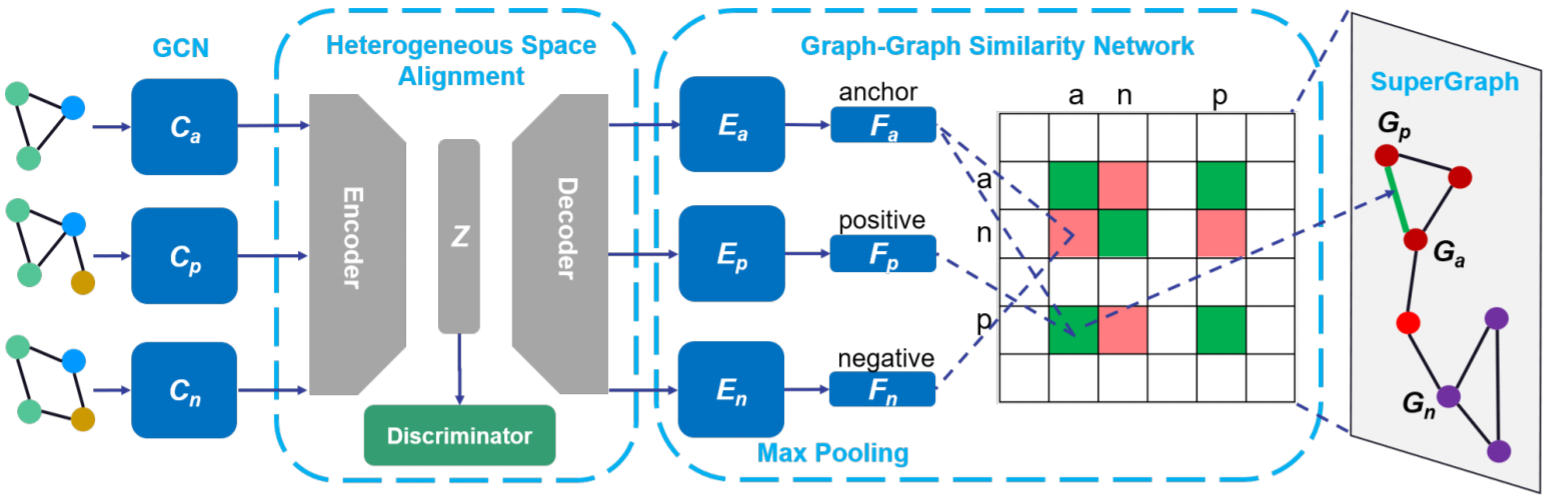
\includegraphics[width=.8\textwidth]{pics/G2G}
	\caption{Overview of Graph-Graph}
	\label{fig:G2G}
\end{figure}

\paragraph{G2G思路}如Fig.\ref{fig:G2G}所示,G2G可以分为四个部分:
\subparagraph{GCN}使用一个共享的GCN为所有的图的结点生成表征。

\subparagraph{Heterogeneous Space Alignment}使用对抗自动编码器\cite{makhzani2016adversarial}用于对生成表征对齐到同一个空间。\tred{这也是我的一个问题,不同的图中的结点的表征所在的空间之间有什么联系呢?}

\subparagraph{Graph-Graph Similarity Network}先通过一个Max pooling来得到图的表征,再基于Contrastive loss和Triplet loss,使用NN来学习图之间的相似性。

\subparagraph{SuperGraph}基于图的表征和相似性矩阵构建一个SuperGraph,每个图都是一个结点,相似性为边的权重。再图表征的基础上,可以使用传统的机器学习方法对SuperGraph中的结点 --- 即原来的图进行分类,论文中使用的是KNN对结点进行分类。
\newline

有一点要注意,G2G每次都使用3个图作为输入,分别是anchor,positive,negative,anchor和positive之间是同类的图,anchor和negative之间是不同类的图,因此在训练过程中使用了Contrastive loss和Triplet loss。

\paragraph{方法解决的问题/优势}
\begin{itemize}
	\item 在完成图分类任务的过程中,学习到了图之间的相似性
	\item 挖掘图的表征空间之间的关系,针对表征空间的问题提出了解决方案,将不同图的表征进行了对齐(\tbc{red}{还有点不太理解文中的意思,原文是:align all the graphs to a same distribution)}
	\item 在对graph-level进行分类时,考虑了图之间的关系(similarity)
	\item 使用triplet进行寻来
\end{itemize}

\paragraph{方法的局限性/未来方向}
\begin{itemize}
	\item 在图类别较多的数据集上效果不是很好
	\item 现有的图分类方法中,主要考虑的是结点的特征和图的拓扑结构,实际中\tbc{red}{边在图中也有很大的作用},进行进行graph-level的任务时,能否考虑边的信息

\end{itemize}
\newline

虽然这篇论文还在双盲中,但我怀疑这篇论文又是\href{http://yunshengb.com/}{Yunsheng Bai}做的。




%\clearpage

\subsection{Deep Graph Similarity Learning: A Survey}
\begin{center}

  \begin{tabular}{rp{6cm}lp{12cm}}%{rl}

  % after \\: \hline or \cline{col1-col2} \cline{col3-col4} ...

  论文地址:& \href{https://arxiv.org/abs/1912.11615}{https://arxiv.org/abs/1912.11615} \\

  %源码:& \href{xxx}{xxx} \\

%  slides:& \href{http://yunshengb.com/wp-content/uploads/2017/03/nips_2018_r2l_workshop_talk.pdf}{{\footnotesize Convolutional Set Matching for Graph Similarity}}\\

  关键词:& \textbf{Metric learning, Graph similarity, GNN} \\

  写于:& \date{2020-10-17}

  \end{tabular}

\end{center}

该论文\cite{ma2020deep}对近年来使用深度学习/GNN计算图相似性的方法进行了一个较为全面的总结,对每种方法进行了一个简要的介绍,描述了图相似性常用的数据集和评估方法,并对图相似性计算的应用及该领域内现存的挑战和难点进行了全面的概括。

图的相似性计算是一种metric learning,学习如何度量两个对象之间的距离。图之间的相似性可以用一个0到1之间的小数表示,但是关键在于如何学习到这样的一个similarity score。

\begin{figure}[h]
	\centering
	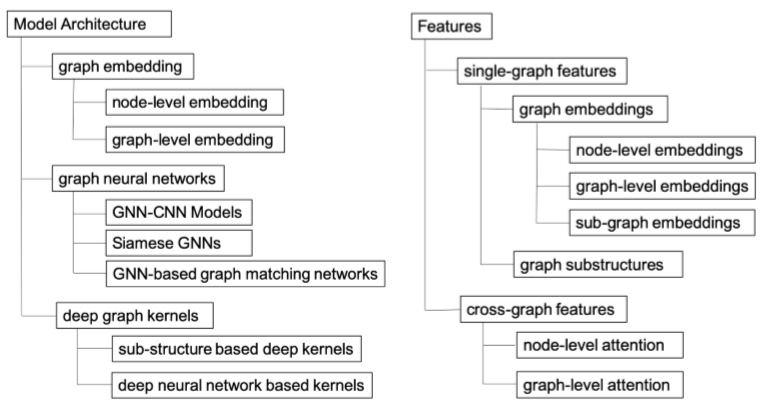
\includegraphics[width=.75\textwidth]{pics/taxonomy_dgs.PNG}
	\caption{Taxonomy of DGS}
	\label{fig:taxonomy_dgs}
\end{figure}

如Fig.\ref{fig:taxonomy_dgs}所示,可以按照模型结构和单/多图的特征来进行分类。按照模型结构,论文中对现有的深度图相似性学习方法主要分为以下三类:
\begin{itemize}
	\item graph-embedding based:使用通过graph embedding方法得到的结点/图表征来计算相似度,如graph2vec,node2vec等
	\item graph neural networks based:在图相似的任务中,以end-to-end的方式使用GNN来学习相似度,如GSimCNN,SimGNN,Siamese GCN等
	\item deep graph kernel based:通过学习核函数来计算同之间的相似性,如Deep graph kernels,Deep divergence graph kernel等
\end{itemize}

论文中对图相似的应用归纳如下:
\begin{itemize}
	\item 在生物信息领域内的应用。例如学习化学元素、分子、化合物等的相似性,研究它们之间的相互作用
	\item 在脑科学中,检测脑网络结构的相似性,分析脑网络的功能。可以指示脑网络功能的正常与否
	\item 计算机安全。可以用来对代码进行分析,
	\item 在计算机视觉中的应用,用于视频序列中动作行为的识别
\end{itemize}

论文中对图相似性的挑战归纳如下:
\begin{itemize}
	\item 在复杂的图数据上的相似性计算。如有向图、动态图/流图、
	\item 解释学习到的结果。
	\item 小样本学习(few-shot learning)。当每一类只有少量数据时如何学习相应的分类器
\end{itemize}

有几个注意的点:
\begin{itemize}
	\item 一个图与自身的相似性要大于等于任何与其他图的相似性,即$s_{ii} >= s_{ij}$
	\item 数据的对齐直觉上是将不同空间/分布的数据放在同一个空间/分布中,但依然能够保持它们原有的某些性质(包括intar,inter的性质)
	\item 在相似性计算时利用结点/边的特征
	\item 由于脑网络的特殊性,脑网络中的相似性更应该是一个子图学习的问题
\end{itemize}
%\paragraph{xxx思路}

%\paragraph{方法解决的问题/优势}
%\begin{itemize}

%	\item 

%\end{itemize}



%\paragraph{方法的局限性/未来方向}

%\begin{itemize}

%	\item 

%\end{itemize}






\subsection{Hierarchical Large-scale Graph Similarity Computation via Graph Coarsening and Matching}
\begin{center}

  \begin{tabular}{rp{6cm}lp{12cm}}%{rl}

  % after \\: \hline or \cline{col1-col2} \cline{col3-col4} ...

  论文地址:& \href{https://arxiv.org/abs/2005.07115}{https://arxiv.org/abs/2005.07115} \\

  %源码:& \href{xxx}{xxx} \\

%  slides:& \href{http://yunshengb.com/wp-content/uploads/2017/03/nips_2018_r2l_workshop_talk.pdf}{{\footnotesize Convolutional Set Matching for Graph Similarity}}\\

  关键词:& \textbf{Graph Similarity, GNN} \\

  写于:& \date{2020-10-18}

  \end{tabular}

\end{center}

该论文\cite{xu2020hierarchical}着眼于大规模图的相似性计算问题。生物/化学中分子识别的时先将分子映射到分子组再在分子组的基础上计算分子的相似性,受到这个启发,论文提出了对大规模图的相似性计算方法 --- COSIM-GNN(Coarsen based Similarity Computation via Graph Neural Network),按照“embedding-coarsening-matching”的过程计算图的相似性。

\begin{figure}[h]
	\centering
	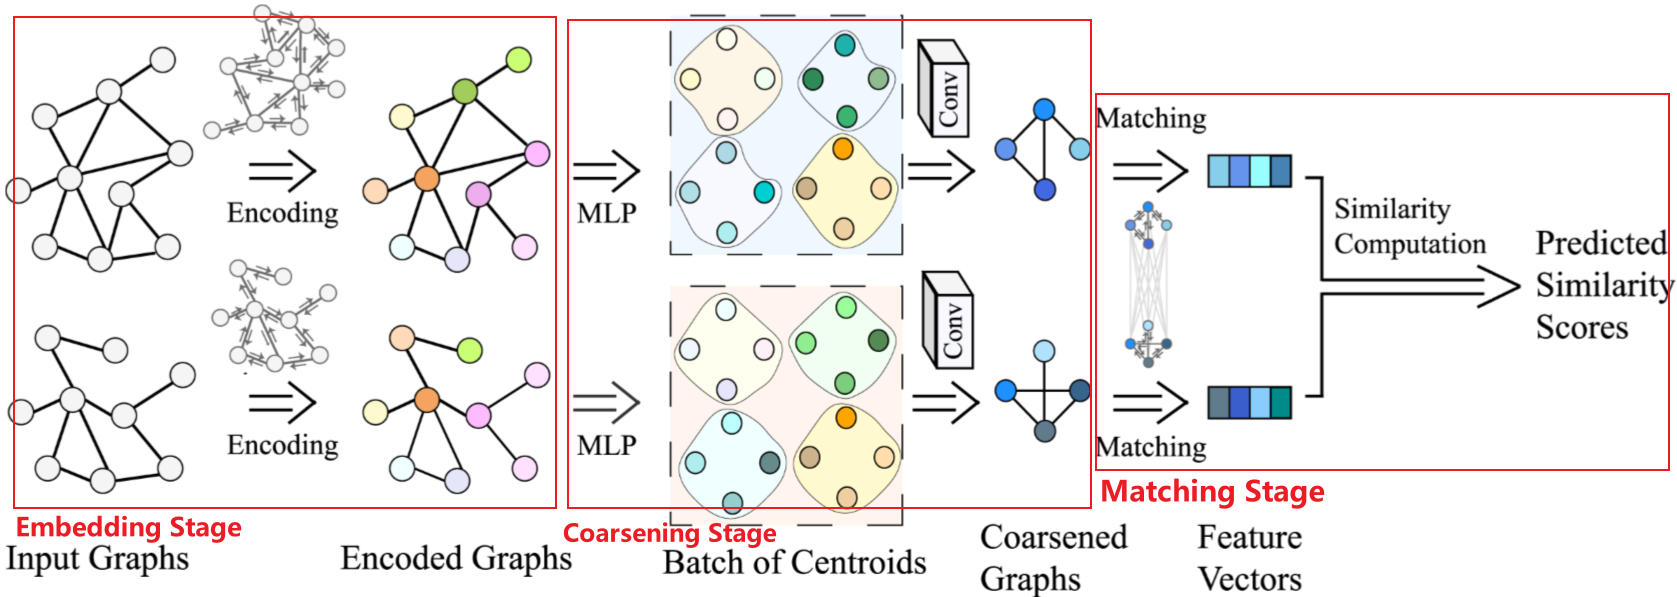
\includegraphics[width=.8\textwidth]{pics/COSIM.PNG}
	\caption{Overview of COSIM-GNN}
	\label{fig:cosim}
\end{figure}

\paragraph{COSIM-GNN思路}整体过程如图Fig.\ref{fig:cosim}所示,可以分为3个阶段:
\subparagraph{Embedding}对输入的两个图,使用GNN分别得到两个图的表征。

\subparagraph{Coarsening}对于Embedding阶段得到的图结点表征,Coarsening阶段,通过池化的方法得到一个粗化后的图。为了使得粗化后的图是和输入数据相关且是节点排列无关的,论文还提出了一个新的池化方法:Adaptive Pooling。该pooling方法在第一阶段的结点表征的基础上得到h个bathch --- 每个batch表示一个不同的图,基于这些batch来获得最终压缩后的图。\tred{为什么要获得h个batch呢?} --- 为了尽量使得到的反映原图的压缩图。具体细节可参看论文(这一部分我没看太懂)。

\subparagraph{Matching}之前的两个阶段中,是分别在输入的两个图上执行这两个阶段。每个图的结果,都只使用了图本身的信息,Matching阶段则涉及到两个图之间的交互,在两个图的基础上一起计算相似性。具体可以使用一些匹配的方法来计算得到它们的相似性,如GSimCNN


\paragraph{方法解决的问题/优势}
\begin{itemize}
	\item 针对大图的相似性计算给出了解决方法
	\item 利用了图之间的信息计算图的相似性,并且通过coarsening降低了这一过程的计算开销
	%\item 

\end{itemize}

\paragraph{方法的局限性/未来方向}
\begin{itemize}
	\item 改进粗化图的方法
	\item 改进图匹配的方法
\end{itemize}


\subsection{Deep Graph Kernels}
\begin{center}

  \begin{tabular}{rp{16cm}lp{20cm}}%{rl}

  % after \\: \hline or \cline{col1-col2} \cline{col3-col4} ...

  论文地址:& \href{https://dl.acm.org/doi/pdf/10.1145/2783258.2783417}{https://dl.acm.org/doi/pdf/10.1145/2783258.2783417} \\
  来源:& KDD’15, Sydney, NSW, Australia \\
  作者:& Pinar Yanardag, S.V.N. Vishwanathan \\
  %源码:& \href{xxx}{xxx} \\

%  slides:& \href{http://yunshengb.com/wp-content/uploads/2017/03/nips_2018_r2l_workshop_talk.pdf}{{\footnotesize Convolutional Set Matching for Graph Similarity}}\\

  关键词:& \textbf{graph kernels, deep learning} \\

  写于:& \date{2020-11-02}

  \end{tabular}

\end{center}

该论文\cite{yanardag2015deep}针对传统的graph kernel方法的缺点提出了Deep Graph Kernels --- 一个能够学习图子结构的潜在表示的统一框架。

\paragraph{使用Graph Kernels计算图相似性}如下公式所示,其中$\phi(\mathcal{G})$表示图$\mathcal{G}$基于子结构的表示向量,例如该向量的每一维表示某一个子结构的出现次数;$\mathcal{M}$表示了所有子结构之间的关系;$\mathcal{K}(G_1, G_2)$是一个核函数,可以用来计算图之间的相似性。
$$
\mathcal{K}(G_1, G_2) = \phi(G_1) \mathcal{M} \phi(G_2)
$$
该论文的重要一点就是学习到子结构的向量表示并计算得到表示这子结构间关系的矩阵$\mathcal{M}$。

传统的graph kernel方法是将图数据(不一定是图,也可以是其他类型的数据,如数、序列等)分解为许多小的子结构,在子结构的基础上就可以将一个图表示为基于子结构的向量。在这些子结构基础上定义有效的核函数(原始特征在高维空间中的内积),就可以使用核函数来计算图之间的相似性。但是传统的graph kernel方法有以下几个缺点:
\begin{itemize}
	\item 通常来说,子结构之间并不是相互独立的。如graphlets(拥有k个结点的,连通的非同构图)。k+1个结点的graphlet包含了k个结点的graphlet
	\item 当图数据很大时,会有很多不同的子结构,图的基于子结构的向量表示将会变得很稀疏。只有一些子结构会出现在图中,在这种情况下,会出现diagonal dominance --- 一个图只与自己相似,与数据集中其他图不相似/相似度很低
\end{itemize}
个人觉得,该论文主要通过神经语言模型的方法学习到子结构的表示,再方便地计算$\mathcal{M}$。但是论文中说的有点含糊。

简单的介绍以下Graph kernels。有很多中Graph kernel,比如基于graphlets的、基于subtree的、基于最短路径的等等,但除了如何生成子结构的方法不同,它们都会用子结构的频数向量来作为图的表示。graph kernels的方法很像language model中的一些方法,如word2vec中的方法。

\paragraph{思路}论文针对不同的Graph kernels 提出了一个统一的框架,能依据子结构之间的依赖性学习子结构的向量表示(即隐表示)。学习隐表示的方法借鉴了神经语言模型中的概念 --- 使用连续的向量表示词使用上下文来定义word。在该论文中,word就是graph kernel,每一个图可以视作sentence,用多个graph kernels即可表示一个图。论文中针对不同的graph kernels方法,使用不同的方法将图分解为子结构的集合。但与语言模型不同的是,一个图生成的子结构间并没有一个明显的共线关系,因此论文中针对不同的graph kernels给出了不同的解决方法 --- 使用不同的方法体现出子结构之间的共现性(也即子结构之间的依赖关系、上下文)。具体怎么产生子结构之间的共现性就不一样描述了,重点是根据graph kernel的特点,衍生出相关的子结构。在生成了子结构以其之间的共现关系后,就可以使用CBOW/Skip-gram算法来学习子结构的向量表示了。之后便可借助子结构的向量表示来计算图之间的相似性了。


\paragraph{方法解决的问题/优势}
\begin{itemize}
	\item 提出了一个统一的框架,能够在不同的graph kernels下学习到子结构的隐表示
	\item 利用graph kernels之间的依赖关系来定义子结构的共现性
\end{itemize}

\paragraph{方法的局限性/未来方向}
\begin{itemize}
	\item 对更复杂的图数据的graph kernels的定义和学习,如attributed graphs
	\item graph kernels方法主要关注的是图的结构信息,不适用于很多真实的图数据
\end{itemize}
}{}

\ifthenelse{\boolean{dynamicgnn}}{
\clearpage
\section{Dynamic Graphs}
\subsection{EvolveGCN: Evolving Graph Convolutional Networks for Dynamic Graphs}
\begin{center}

  \begin{tabular}{rp{16cm}lp{20cm}}%{rl}

  % after \\: \hline or \cline{col1-col2} \cline{col3-col4} ...

  论文地址:& \href{https://arxiv.org/pdf/1902.10191}{https://arxiv.org/pdf/1902.10191} \\
  来源:& AAAI, 2020 \\
  作者:& Pareja, Aldo, et al. \\
  源码:& \href{https://github.com/IBM/EvolveGCN}{EvolveGCN} \\

%  slides:& \href{http://yunshengb.com/wp-content/uploads/2017/03/nips_2018_r2l_workshop_talk.pdf}{{\footnotesize Convolutional Set Matching for Graph Similarity}}\\

  关键词:& \textbf{Dynamic Graphs, GCN} \\

  写于:& \date{2021-02-17}

  \end{tabular}

\end{center}

该论文\cite{pareja2019evolvegcn}解决的是不断进化(evolve)的graph的表征问题。以往的方法主要将结点的表征通过RNN来学习不断进化的graph,这种方法在学习表征时需要知道结点在所有时间区间上的变化(相当于是transductive的),并且在变化比较频繁的graph上不太友好。论文提出EvolveGCN,将GCN和RNN结合,使用RNN来学习GCN的参数,以此来捕捉动态图的动态性。

\paragraph{问题定义}
对于一个动态图$G$,在每一个时间点$t$上,可以将$G$表示为$(A_t,X_t)$,分别表示时间$t$时的邻接矩阵和特征矩阵。最终要学习的是$G$中每个结点在各个时间点上的结点表征。

\begin{figure}[h]
	\centering
	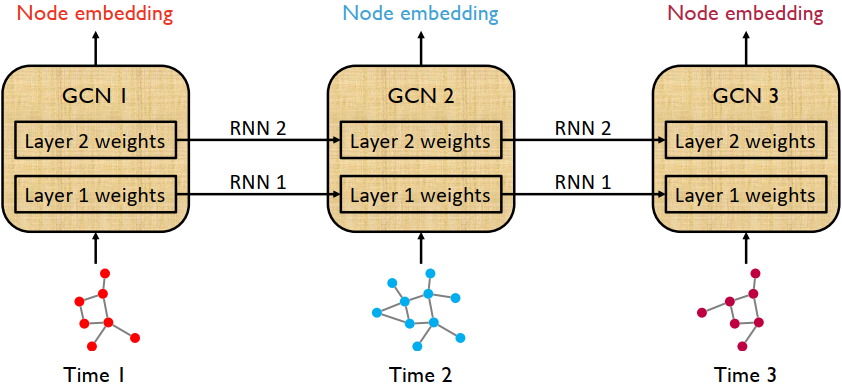
\includegraphics[width=.8\textwidth]{pics/EvolveGCN.png}
	\caption{EvolveGCN}
	\label{fig:evolvegcn}
\end{figure}

\paragraph{EvolveGCN思路}
如Fig.\ref{fig:evolvegcn}所示,在时间点$t$时,将$(A_t,X_t)$输入到模型中,可以学习到$t$时的结点表征。注意,\tbc{red}{GCN的参数并不是训练得来的,而是通过RNN计算得到的}。GCN在EvolveGCN中起的作用:通过$(A_t,X_t)$得到结点表征,但是并不会在计算表征的过程中更新GCN各层的参数。RNN在EvolveGCN中起的作用:在$t-1$时的结点表征和GCN参数的基础上更新GCN的参数,更新公式如下:
$$
\overbrace{\underbrace{W_{t}^{(l)}}_{\text {hidden state }}}^{\text {GCN weights }}=\operatorname{GRU}(\underbrace{\overbrace{H_{t}^{(l)}}^{\text {node embeddings }}}_{\text {input }}, \overbrace{\underbrace{W_{t-1}^{(l)}}_{\text {hidden state }}}^{\text {GCN weights }})
$$
或
$$
\overbrace{\underbrace{W_{t}^{(l)}}^{\text {GCN weights }}}_{\text {output }}=\operatorname{LSTM}(\overbrace{\underbrace{W_{t-1}^{(l)}}_{\text {input }}}^{\text {GCN weights }})
$$
从上可以得到,动态图的变化都保存在了GCN的参数中。在实现时,需要对RNN进行更改:
\begin{itemize}
	\item 将RNN单元的输入与隐状态扩展为矩阵形式,因为GCN的参数和结点表征都是矩阵的形式
	\item 将输入的列与隐状态的列相匹配
\end{itemize}


\paragraph{方法解决的问题/优势}
\begin{itemize}

	\item 对动态图的表征学习提出了可行的解决方法
	\item 将RNN和GCN相结合,利用RNN来进化GCN的参数,能够应对变化频繁的graph,而且不需要提前预知结点的所有变化

\end{itemize}


\paragraph{方法的局限性/未来方向}

\begin{itemize}
	\item 虽然不需要提前预知结点的所有变化,但是\tbc{red}{需要预知graph中的所有结点,不能应对结点的变化}
	\item 使用RNN来进化GCN的参数,将graph的动态性保存在参数中,一个训练好的模型也许只能捕捉一种动态性

\end{itemize}





\subsection{Temporal Graph Networks for Deep Learning on Dynamic Graphs}
\begin{center}

  \begin{tabular}{rp{16cm}lp{20cm}}%{rl}

  % after \\: \hline or \cline{col1-col2} \cline{col3-col4} ...

  论文地址:& \href{https://arxiv.org/pdf/2006.10637.pdf}{https://arxiv.org/pdf/2006.10637.pdf} \\
  来源:& ICML 2020 Workshop \\
  作者:& Emanuele Rossi, et al. \\
  源码:& \href{https://github.com/twitter-research/tgn}{tgn} \\
  slides:& \href{https://www.emanuelerossi.co.uk/assets/pdf/tgn_aisc_2020.pdf}{TGN: Temporal Graph Networks for Dynamic Graphs} \\
  关键词:& \textbf{graph representation, temporal graph} \\
  写于:& \date{2021-03-01}

  \end{tabular}

\end{center}

该论文\cite{rossi2020temporal}主要解决的是连续时间下的动态图的表示,论文中将连续时间下的动态图看成流图 --- 由一系列的带时间戳的事件组成。

\paragraph{问题定义}
论文中将动态图建模为带时间戳的事件序列:$\mathcal{G}=\left\{x\left(t_{1}\right), x\left(t_{2}\right), \ldots\right\}$。事件$x(t)$有两种类型:1)结点事件,新增一个结点或者更新一个结点的特征,用$\mathbf{v}_i(t)$表示;2)交互事件:表示结点之间的交互,由$\mathbf{e}_{i j}(t)$表示。该论文的主要贡献就是建立了一个通用的框架来对动态图进行建模,并且将一系列的模块组合起来对动态图进行学习,得到结点在某个时间点上的表征。\textbf{将TGN作用在一个连续时间的动态图上,将为每个结点在每个时间点上产生一个表征}。

\paragraph{TGN思路}
简言之,TGN可以看作一个编码器,共由5个子模块组成。

\subparagraph{Memory}
$t$时的模型的Memory由模型到$t$时为止所见到的结点$i$的状态$\mathbf{s}_i(t)$组成。结点的状态相当于对结点的历史信息的一个压缩形式的表示。

\subparagraph{Message Function}
$t$时,当有涉及$i$结点的事件时,一条message会被计算用于更新$i$的状态。论文中对两种事件的消息计算公式如下:
$$
\mathbf{m}_i(t) = msg_s(\mathbf{s}_i(t^{-}), \mathbf{s}_j(t^{-}), \triangle t, \mathbf{e}_{ij}(t))
$$
$$
\mathbf{m}_j(t) = msg_d(\mathbf{s}_j(t^{-}), \mathbf{s}_i(t^{-}), \triangle t, \mathbf{e}_{ij}(t))
$$
$$
\mathbf{m}_i(t) = msg_n(\mathbf{s}_i(t^{-}), t, \mathbf{v}_{i}(t))
$$

$msg_s, msg_t, msg_n$分别表示交互事件中源节点和目标节点、结点事件中所涉及的结点的消息的计算公式。具体实现时可以有多种形式,如MLP,在论文中采用的是拼接的形式。

\subparagraph{Message Aggregator}
由于在实际中通常会采用一次性处理多个事件(可能是多个时间的多个事件),需要将多个事件对应的message汇聚,形式如下:
$$
\bar{\mathbf{m}}_i(t) = agg(\mathbf{m}_i(t_1), ..., \mathbf{m}_i(t_b))
$$
$agg$的具体实现形式也可以是多样的,如RNN、mean等,论文中采用的是只选择最近的message。

\subparagraph{Memory Updater}
得到了$t$时设计到$i$的message后就可以更新状态了。
$$
\mathbf{s}_i(t) = mem(\bar{m}_i(t), \mathbf{s}_i(t^-))
$$
同样,$mem$的形式也可以是多样的,如LSTM、GRU等。

\subparagraph{Embeddings}
这个模块是用于为$i$生成在$t$时的表征的:
$$
\mathbf{z}_i(t) = emb(i, t) = \sum_{j \in N_i^k([0, t])} h(\mathbf{s}_i(t), \mathbf{s}_j(t), \mathbf{e}_{ij}, \mathbf{v}_i(t), \mathbf_{v}_j(t))
$$
$h$的具体形式也是多样的。

最终TGN的整体如Fig.\ref{fig:tgn}所示。
\begin{figure}[h]
	\centering
	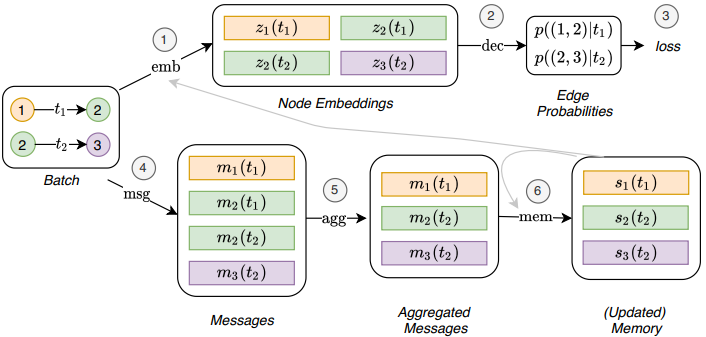
\includegraphics[width=.8\textwidth]{pics/TGN.png}
	\caption{TGN}
	\label{fig:tgn}
\end{figure}



\paragraph{方法解决的问题/优势}

\begin{itemize}

	\item 对连续时间下的动态图进行了建模,以事件序列表示一个动态图
	\item 对动态图的表征学习提出了一个统一的框架
	\item 可应用于异常检测、金融交易等场景中
	
\end{itemize}



\subsection{Inductive representation learning on Temporal Graphs}
\begin{center}

  \begin{tabular}{rp{16cm}lp{20cm}}%{rl}

  % after \\: \hline or \cline{col1-col2} \cline{col3-col4} ...

  论文地址:& \href{https://openreview.net/pdf?id=rJeW1yHYwH}{https://openreview.net/pdf?id=rJeW1yHYwH} \\
  来源:& ICLR, 2020\\
  作者:& Da Xu, Chuanwei Ruan, et al. \\

  源码:& \href{https://github.com/StatsDLMathsRecomSys/Inductive-representation-learning-on-temporal-graphs}{TGAT} \\

%  slides:& \href{http://yunshengb.com/wp-content/uploads/2017/03/nips_2018_r2l_workshop_talk.pdf}{{\footnotesize Convolutional Set Matching for Graph Similarity}}\\

  关键词:& \textbf{self-attention mechanism, graph representation, temporal graph} \\

  写于:& \date{2021-03-01}

  \end{tabular}

\end{center}

该论文\cite{tgat_iclr20}也是为了解决动态图的表征问题。改论文在self-attention\cite{vaswani2017attention}机制的基础上,提出了temporal graph attention(TGAT) layer来汇集temporal-topological neighborhood features。

\paragraph{问题定义}
该论文讨论的也是连续时间下的动态图的表征问题,与\cite{rossi2020temporal}不同,该论文并没有将动态图用事件序列来表示,重点关注的时图中结点的temporal neighborhoods,如何利用temporal neighborhoods来计算结点在$t$时的表征。

\paragraph{TGAT思路}
在介绍TGAT之前,先来了解以下self-attention是啥。
\subparagraph{self-attention}
简单的来说自注意力机制就是输入一个序列的数据,以序列自身来计算序列中各个元素与其他元素(包括自身)之间的关系大小(注意力大小)。self-attention最开始用于自然语言处理中。在计算自注意力时需要将位置编码与序列中元素的表征相结合。
$$
Attn(Q, K, V) = softmax(\frac{\mathbf{Q}\mathbf{K}^\intercal}{\sqrt{d}}) \mathbf{V}
$$
上式中的$\mathbf{Q,K,V}$都是由同一个矩阵$\mathbf{X}$(表征矩阵)乘以不同的权重矩阵得到的。

\subparagraph{TGAT}
TGAT中将self-attention中的positional encoding替换为time encoding,再将time encoding与结点特征相结合构成Temporal Graph Attention Layer。time encoding的输入为时间戳,输出为一个向量。对于时间$t$,结点$i$的temporal neighborhoods包括在时间$t$之与$i$发生了交互(即存在过边)的结点,每个结点上一层的表征和时间表征拼接起来作为self-attention中的$\mathbf{X}$,即可计算得到当前节点与其temporal neighborhoods之间的注意力,邻居结点的上一层的表征加权求和后隐表示,该隐表示再与结点的特征向量拼接后输入到MLP中,最终的输出为节点在$t$时的TGAT层输出。TGAT layer如Fig.\ref{fig:tgat}所示。

\begin{figure}[h]
	\centering
	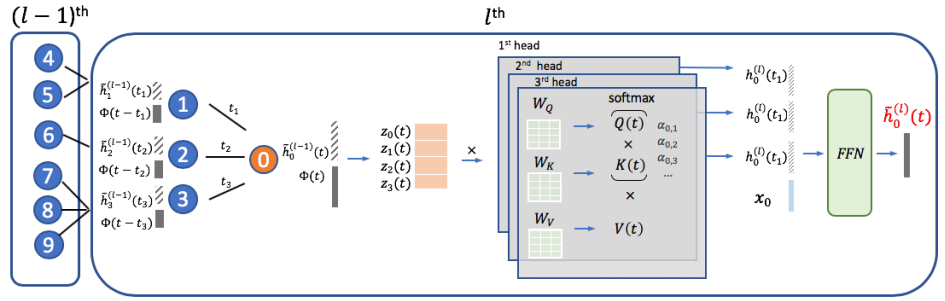
\includegraphics[width=.8\textwidth]{pics/TGAT.png}
	\caption{TGAT layer,采用了多头注意力机制,k=3}
	\label{fig:tgat}
\end{figure}

说实话,TAGT的大概意思看懂了,但是其中涉及time encoding转化为一个分布学习的问题、TGAT layer的具体实现过程不是很懂。






\paragraph{方法解决的问题/优势}

\begin{itemize}

	\item 引入了temporal的图注意力机制
	\item 将self-attention中的positional encoding替换为time encoding
	\item 引入了注意力机制能够增加模型的可解释性

\end{itemize}



\paragraph{方法的局限性/未来方向}

\begin{itemize}

	\item 对于$t$时的结点的表征,需要考虑$t$之前的所有相关邻居,如果$t$很大时可能会存在计算开销很大的问题
	\item 结点的特征已经在第一层输入了,但是在TGAT层中还将节点特征与隐表征拼接后输入到FFN中,这样是否有必要?

\end{itemize}





\subsection{DySAT: Deep Neural Representation Learning on Dynamic Graph via Self-Attention Networks}
\begin{center}

  \begin{tabular}{rp{16cm}lp{20cm}}%{rl}

  % after \\: \hline or \cline{col1-col2} \cline{col3-col4} ...

  论文地址:& \href{http://yhwu.me/publications/dysat_wsdm20.pdf}{http://yhwu.me/publications/dysat\_wsdm20.pdf} \\
  来源:& WSDM, 2020\\
  作者:& Aravind Sankar, Yanhong Wu, et al. \\
  源码:& \href{https://github.com/aravindsankar28/DySAT}{DySAT} \\

%  slides:& \href{http://yunshengb.com/wp-content/uploads/2017/03/nips_2018_r2l_workshop_talk.pdf}{{\footnotesize Convolutional Set Matching for Graph Similarity}}\\

  关键词:& \textbf{self-attention, representation learning, dynamic graphs} \\

  写于:& \date{2021-03-02}

  \end{tabular}

\end{center}

该论文\cite{sankar2020dysat}解决的是动态图中的结点表征问题。论文提出了DySAT(Dynamic Self-Attention),以自注意力机制捕捉动态图的结构的动态性。DySAT分别从两个方面捕捉动态性:structural neighborhoods和temporal dynamics,并且使用多头注意力来捕捉多方面的动态性。

\paragraph{问题定义}
论文中使用图序列来表示动态图。关于动态图的建模,在这里插一句。

\subparagraph{dynamic graph}
动态图通常由两种建模方式:图序列(graph snapshots)和基于带时间戳的事件的图(time stamped events,类似于流图)。本质上来看这两种建模方式是等价的,是可以互相转化的。但是不同的建模形式针对这不同的应用场景。snapshot形式的动态图,直观上强调的整体性,图中结点/边的变化是为了整体的图而服务的,这种情况下我们更多的考虑的是作为一个整体的图的应用场景,例如在场景识别中、对图进行分类的任务中。而timestamped形式的动态图,对整体的考虑可能会不是那么强,更强调的是图中结点/边以及这些变化对任务的影响。

作者采用的是snapshots形式的动态图$\mathbb{G} = \{\mathcal{G}^1, ..., \mathcal{G}^T\}$。其中$T$是时间步的数量,$\mathcal{G}^t = (\mathcal{V}, \mathcal{E}^t)$。显然,该论文中动态图的结点是不变的,即\tbc{red}{不涉及结点的增加或删除}。最终的目标就是学习图中每个结点在任意时间$t$时的表征。

\paragraph{DySAT思路}
\begin{figure}[h]
	\centering
	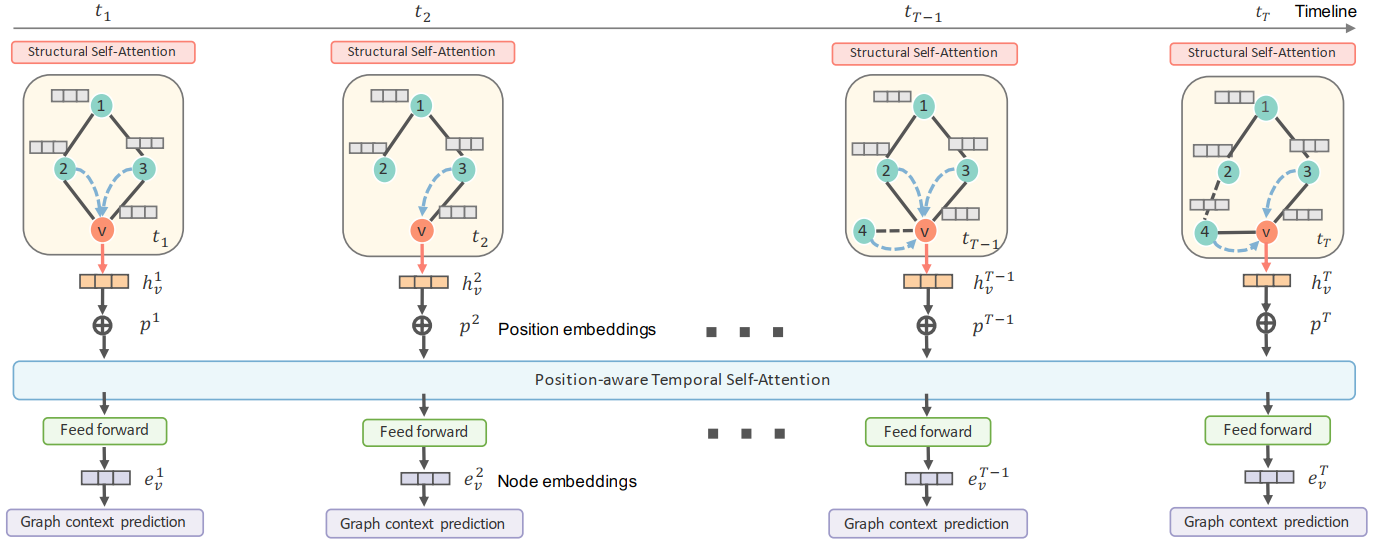
\includegraphics[width=.8\textwidth]{pics/DySAT.png}
	\caption{DySAT}
	\label{fig:dysat}
\end{figure}
DySAT的整体框架如Fig.\ref{fig:dysat}所示。DySAT主要分为两个部分:Structural Self-Attention和Temporal Self-Attention。

\subparagraph{Structural Self-Attention}
这一部分与GAT中的注意力机制类似,想当于一个邻居结点信息汇聚层。对于每一个snapshot graph,Structural Self-Attention利用当前时刻各个结点的表征计算注意力再进行加权求和,计算公式如下:
$$
\begin{array}{c}
	z_{v}=\sigma\left(\sum_{u \in \mathcal{N}_{v}} \alpha_{u v} W^{s} x_{u}\right), \alpha_{u v}=\frac{\exp \left(e_{u v}\right)}{\sum_{w \in \mathcal{N}_{v}} \exp \left(e_{w v}\right)} \\
	e_{u v}=\sigma\left(A_{u v} \cdot \boldsymbol{a}^{T}\left[\boldsymbol{W}^{s} \boldsymbol{x}_{u} \| \boldsymbol{W}^{s} \boldsymbol{x}_{v}\right]\right) \forall(u, v) \in \mathcal{E}
\end{array}
$$

\subparagraph{Temporal Self-Attention}
这部分是为了捕捉动态图在时间上的变化模式。计算结点$v$在$t$时的表征时,将在$t$之前的$v$的表征作为temporal self-attention模块的输入,输出的是结点$v$在各个事件点的表征(此时的表征考虑了动态性),计算公式如下:
$$
\begin{array}{r}
	Z_{v}=\beta_{v}\left(X_{v} W_{v}\right), \quad \beta_{v}^{i j}=\frac{\exp \left(e_{v}^{i j}\right)}{\sum_{k=1}^{T} \exp \left(e_{v}^{i k}\right)} \\
	e_{v}^{i j}=\left(\frac{\left(\left(X_{v} W_{q}\right)\left(X_{v} W_{k}\right)^{T}\right)_{i j}}{\sqrt{F^{\prime}}}+M_{i j}\right)
\end{array}
$$
上式的形式与self-attention的形式一致。其中的$\mathbf{M} \in \mathbb{R}^{T \times T}$是一个掩码矩阵,
$$
M_{i j}=\left\{\begin{array}{ll}
	0, & i \leq j \\
	-\infty, & \text { otherwise }
\end{array}\right.
$$

通常一个注意力捕捉的是一个方面的性质,为了捕捉动态图中多个方面的动态性,作者引入了多头注意力,Structural和Temporal都引入了多头注意力机制。

为了训练模型中的参数,论文使用类似神经语言模型中的共现率来优化参数,这点与word2vec和Node2vec中的损失函数很像,损失函数如下,$P_n^t$为负采样的结点:
$$
\begin{aligned}
	L=\sum_{t=1}^{T} \sum_{v \in \mathcal{V}}\left(\sum_{u \in \mathcal{N}_{\text {walk }}^{t}(v)}-\log \left(\sigma\left(<\boldsymbol{e}_{u}^{t}, \boldsymbol{e}_{v}^{t}>\right)\right)\right.\\
	&\left.-w_{n} \cdot \sum_{u^{\prime} \in P_{n}^{t}(v)} \log \left(1-\sigma\left(<\boldsymbol{e}_{u^{\prime}}^{t}, \boldsymbol{e}_{v}^{t}>\right)\right)\right)
\end{aligned}
$$

DySAT是先进行structural self-attention再进行temporal self-attention,作者这样设计是因为:随着时间变化,图的结构是不稳定的。

\paragraph{方法解决的问题/优势}

\begin{itemize}

	\item 提出了structural和temporal self-attention来学习动态图中的结点表征
	\item 使用多头注意力机制捕捉多方面的动态性
	\item 注意力机制适用于并行

\end{itemize}

\paragraph{方法的局限性/未来方向}

\begin{itemize}

	\item 只能适用于结点不变化的动态图
	\item 以结点的共现率为损失函数引导模型的训练,这样的损失函数可能重点关注的是图的结构,对于动态性更丰富的图(如结点的特征的变化)是不够的

\end{itemize}




\subsection{Spatial Temporal Graph Convolutional Network for Skeleton-Based Action Recogonition}
\begin{center}

  \begin{tabular}{rp{16cm}lp{20cm}}%{rl}

  % after \\: \hline or \cline{col1-col2} \cline{col3-col4} ...

  论文地址:& \href{https://arxiv.org/pdf/1801.07455.pdf}{https://arxiv.org/pdf/1801.07455.pdf} \\
  来源:& AAAI, 2018\\
  作者:& Sijie Yan, Yuanjun Xiong, Dahua Lin \\

  源码:& \href{https://github.com/yysijie/st-gcn}{st-gcn} \\

%  slides:& \href{http://yunshengb.com/wp-content/uploads/2017/03/nips_2018_r2l_workshop_talk.pdf}{{\footnotesize Convolutional Set Matching for Graph Similarity}}\\

  关键词:& \textbf{Action Recogonition, GCN} \\

  写于:& \date{2021-03-04}

  \end{tabular}

\end{center}
$
\displaystyle
\int_{\partial\text{\emoji{hourglass}}} \text{\emoji{frog}}
= \int_\text{\emoji{hourglass}} \mathrm{d}\text{\emoji{frog}}
$

该论文\cite{yan2018spatial}针对人体动作识别问题提出了解决方案。以Skeleton为基础构建时空图,提出了ST-GCN(Spatial Temporal GCN)对人体行为的时空图进行表征,在进行行为分类。

\paragraph{问题定义}
给定一段视频,确定其中的人体行为类别。可以从多个方面表示人体行为,如光流、骨骼关键点等,该论文中采用基于骨骼关键点的形式表示人体行为。在一段视频中,每一帧中的人体骨骼点可以构成一个graph --- Spatial graph,帧与帧之间同一个骨骼点进行连接可以构成graph --- Temporal graph。论文的目标就是基于一个视频的骨骼点构成的Spatial Temporal graph来对人体行为进行分类。

\paragraph{ST-GCN思路}
\begin{figure}[h]
	\centering
	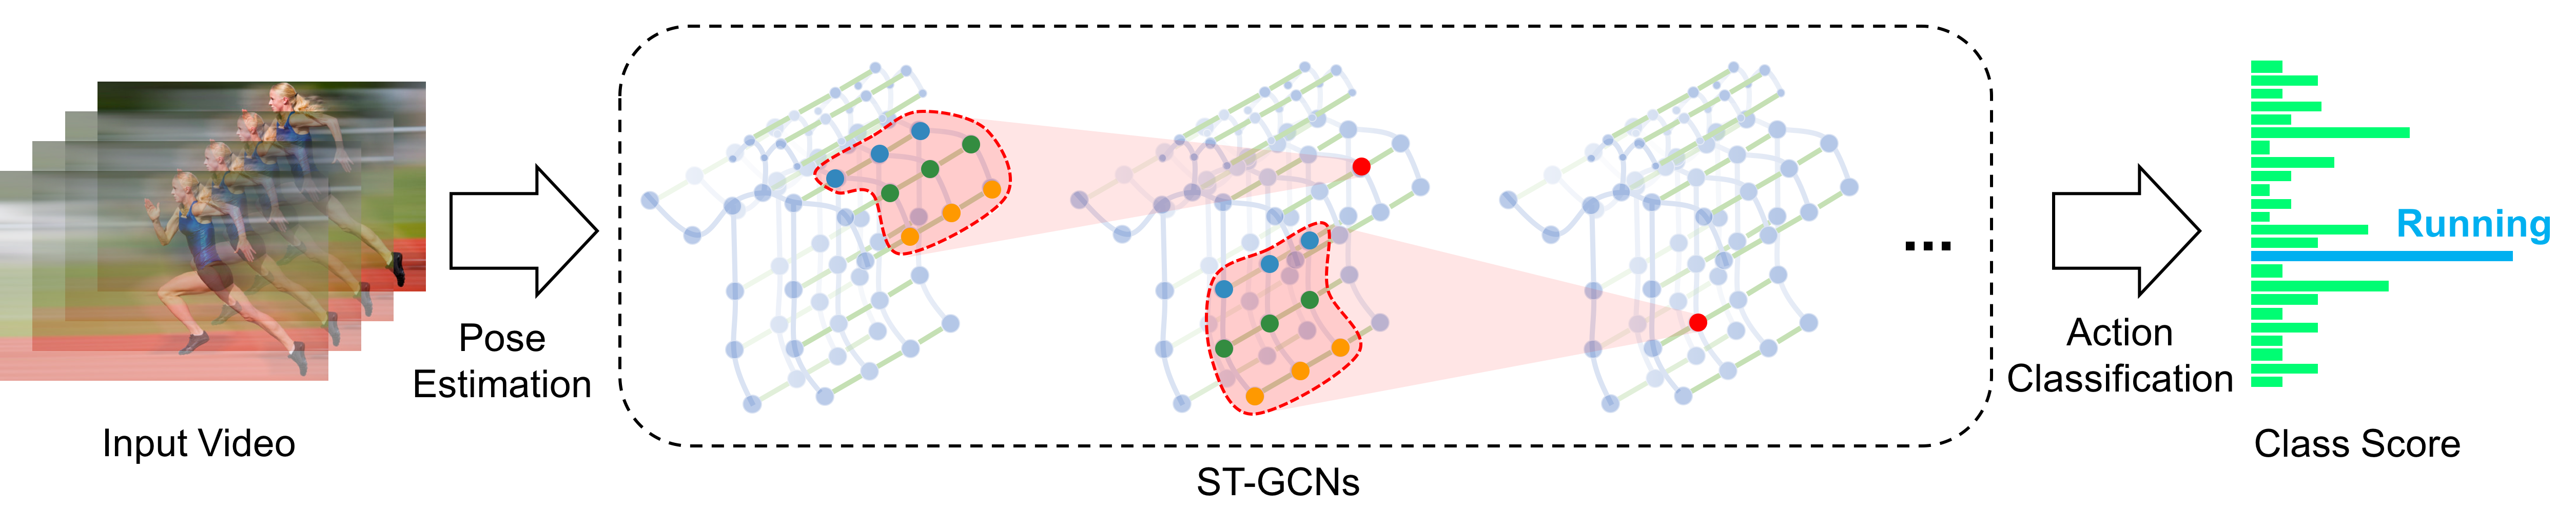
\includegraphics[width=.8\textwidth]{pics/ST-GCN.png}
	\caption{ST-GCN}
	\label{fig:st-gcn}
\end{figure}
\subparagraph{Skeleton Graph Construction}
Spatial Temporal Graph $G = (V, E)$,$V = \{v_{ti} | t=1, ..., T, i = i, ..., N\}$中的结点来自人体骨骼关键点,$N$表示关键点个数,$T$表示视频帧数。每一帧中的Graph构建以人体自然连接为依据,帧与帧之间的Graph构建方式为:相邻帧之间,同一个关键点进行相连。因此,边也分为两种:$E_S = \{v_{ti}v_{tj} | (i,j) \in H\}, E_F = \{v_{ti}v_{(t+1)i}\}$,其中$H$表示人体中关键点的自然连接。

\subparagraph{Spatial Graph Convolutional Neural Network}
作者在Spatial Temporal Graph的基础上定义了Spatial Temporal Convolution。这个卷积操作与GCN中的卷积很类似,但是加上了一个时间维度 --- 每个结点的邻居不仅要考虑当前帧中相邻的结点还要考虑时间上相邻帧的连接。对于图中每个结点,其特征为骨骼关键点在帧中的位置。

经过多层的Spatial Temporal Convolution后,将特征输入到MLP中进行行为分类即可。

\paragraph{方法解决的问题/优势}

\begin{itemize}

	\item 首次将GCN应用于行为识别
	\item 不仅考虑了帧中各个关键点,还考虑了帧间关键点

\end{itemize}

\paragraph{方法的局限性/未来方向}

\begin{itemize}

	\item 论文中提到的注意力机制没有明显的意义
	\item 只考虑了局部特征

\end{itemize}





\subsection{Inductive Representation Learning In  Temporal Networks via Causal Anonymous Walks}
\begin{center}

  \begin{tabular}{rp{16cm}lp{20cm}}%{rl}

  % after \\: \hline or \cline{col1-col2} \cline{col3-col4} ...

  论文地址:& \href{https://arxiv.org/pdf/2101.05974.pdf}{https://arxiv.org/pdf/2101.05974.pdf} \\
  来源:& ICLR, 2021 \\
  作者:& Yanbang Wang, et al. \\

  源码:& \href{https://github.com/snap-stanford/CAW}{CAW} \\

%  slides:& \href{http://yunshengb.com/wp-content/uploads/2017/03/nips_2018_r2l_workshop_talk.pdf}{{\footnotesize Convolutional Set Matching for Graph Similarity}}\\

  关键词:& \textbf{Link Prediction, Causal Anonymous Walk, Temporal Graph} \\

  写于:& \date{2021-03-09}

  \end{tabular}

\end{center}

该论文\cite{wang2021inductive}就动态网络的模式抽取问题,针对现有方法中的一些弊端:如主要依靠结点id和丰富的边的属性且难以抽取复杂的模式,提出了CAW(Cusal Anonymous Walk)以inductive的形式表示动态图。CAW也是一种游走,在Temporal networks中以anonymization的策略游走生成CAWs,将这些CAWs作为motifs来表示动态网络。CAWs不需要传统的基于核方法中的选择什么样的motifs、统计motifs个数不同。再者,论文中提出了神经网络模型CAW-N用于编码CAWs。

\paragraph{问题定义}
动态网络中存在众多的模式,例如三角闭包以及一些更复杂的模式,目标就是在动态网络的表示中能够包含这些复杂的模式。当前对与动态网络的表示只能表示一些简单的模式或者主要停留在静态网络上。对于动态网络的研究主要由三个挑战:1)动态网络中结构和时序的混合,需要一个更好的模型对动态网络进行建模;2)模型的伸缩性,动态网络会不断地被新到来的数据更新;3)能够学习训练数据中出现过的数据,并提取出它的模式。

这里介绍一下inductive和transductive:Transduction is reasoning from obeserved, specific (training) cases to specific (test) cases. In contrast, induction is reasoning from obeserved training cases to gerneral rules, which are then applied to the test cases.

论文中用$\mathcal{E}=\{(e_1, t_1), (e_2, t_2), ...\}$表示动态网络,其中的含义显然易见。这个序列的边就编码的网络的动态性,那么,\textbf{动态网络的表示模型的表示能力就取决于能否准确地基于以往的信息预测结点之间的连接}。论文中也使用链接预测来作为模型的指标。

再介绍一些用到的符号:$\mathcal{E}_{v, t}=\left\{\left(e, t^{\prime}\right) \in \mathcal{E} \mid t^{\prime}<t, v \in e\right\}$表示在$t$之前与$v$相连的边集;下式表示一个CAW,注意其中时间使从大到小的,及新的边放在前面,$W[i]$表示第$i$个结点-时间对。
$$
W=\left(\left(w_{0}, t_{0}\right),\left(w_{1}, t_{1}\right), \ldots,\left(w_{m}, t_{m}\right)\right), t_{0}>t_{1}>\cdots>t_{m},\left(\left\{w_{i-1}, w_{i}\right\}, t_{i}\right) \in \mathcal{E} \text { for all }
$$

\paragraph{CAW思路}
在CAW之前有Anonymous walks(AW)\cite{micali2016reconstructing},如Fig.\ref{fig:aw}所示,AW很像随机游走,但是又与之有点不同 --- 用结点在walks中出现的顺序替代结点的id。这里也给我一个较大的启示:\tbc{red}{实践中对结点的编号并不能体现graph中的模式,在学习模式的表征时,应尽可能将实践时引入的编号等一些辅助信息与graph的结构、模式等区分开来。但是在实践时有时需要一个明确的表示的,可以借助一个中间的表示,将在不同应用场景下的表示转化为中间表示,用中间表示来表示模式。这有点类似于虚拟机和神经机器翻译中的概念}。
\begin{figure}[h]
	\centering
	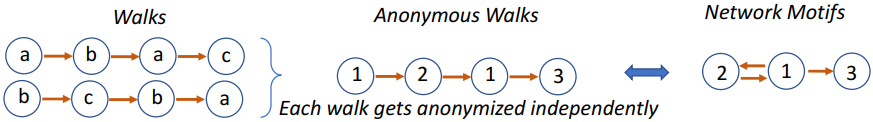
\includegraphics[width=.8\textwidth]{pics/AW.png}
	\caption{Anonymous walks}
	\label{fig:aw}
\end{figure}

CAW中就采用了这种思想,将结点的编号用结点在某个特定位置出现的次数代替。对于给定的两个结点,当预测它们的边时,需要先分别以这两个结点为起点抽取CAWs,再用论文中的方法替换结点的编号,再分别对walks进行编码,最后在预测边的概率。论文中提出的CAW-N主要由以下这些部分组成。
\subparagraph{Causal Anonymous Walk}
\textbf{Causal Anonymous Walk}由两部分组成:\textbf{Causality Extraction}和\textbf{Set-based Anonymization},如Fig.\ref{fig:caw}所示。

\begin{figure}[h]
	\centering
	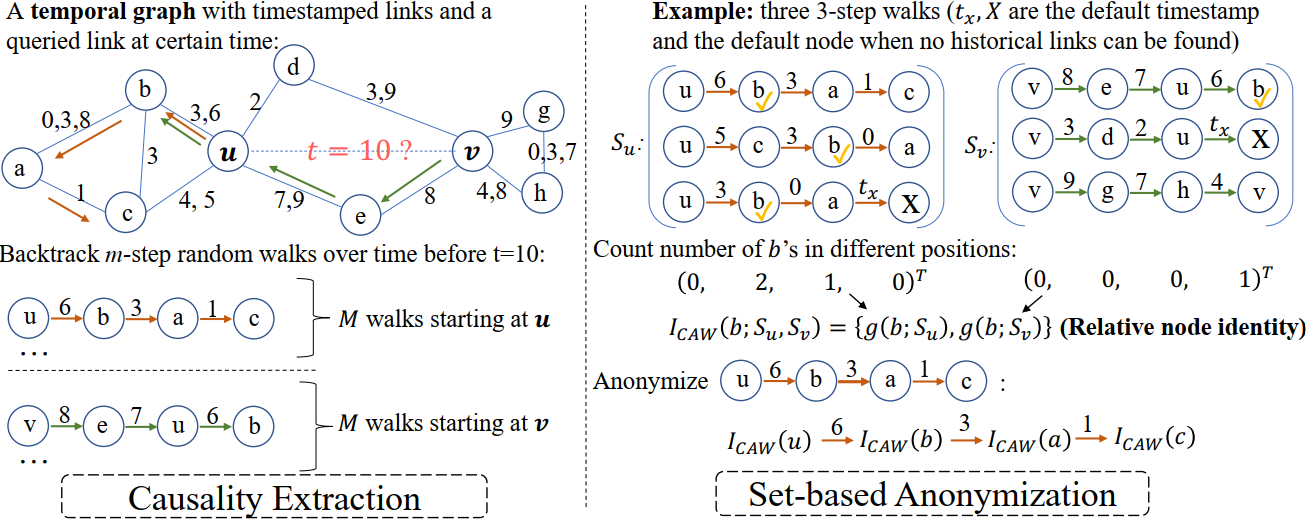
\includegraphics[width=.8\textwidth]{pics/CAW.png}
	\caption{CAW}
	\label{fig:caw}
\end{figure}

Causality Extraction这一部分主要用于从动态网络中抽取出walks(这个时候还不能称为Causal Anonymous Walks),抽取算法如Fig.\ref{fig:caw-walk-eatraction}所示。
\begin{figure}[h]
	\centering
	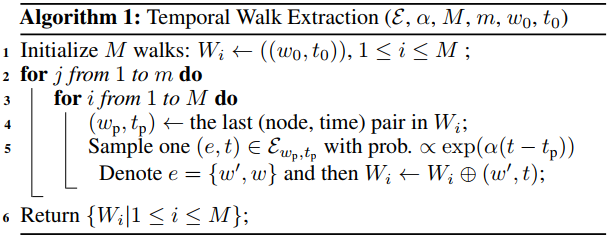
\includegraphics[width=.75\textwidth]{pics/CAW-Walk-Extraction.png}
	\caption{Temporal Walk Extraction}
	\label{fig:caw-walk-eatraction}
\end{figure}
对于结点$u_0, v_0$,该算法会分别以$u_0, v_0$为起点得到长度为$m$的$M$条CAWs,分别为$S_u, S_v$。得到walks后,需要将中的结点id去掉,转化成“中间表示”。转换过程就由Set-based Anonymization完成。

这一部分就是将walks中的结点id $w$转化为相对结点id $I_{CAW}(w; \{S_u,S_v\})$。\cite{micali2016reconstructing}中只是基于一条路径进行转换,这是基于一个假设:任意两个AWs不会共享结点id。显然,该论文中的转换是基于$2M$条CAWs转换的,这也是基于一个假设:\textbf{CAWs之间的关系可能是动态图中模式的关键之处}。因此共享结点id的CAWs就相当于保留了这种关系。$I_{CAW}(w; \{S_u,S_v\})$定义如下。
$$
I_{C A W}\left(w ;\left\{S_{u}, S_{v}\right\}\right) \triangleq\left\{g\left(w, S_{u}\right), g\left(w, S_{v}\right)\right\}
$$
对于$w_0 \in \{u, v\}$,$g(w, s_{w_0}) \in \mathbb{Z}^{m+1}$表示$w$在集合$S_{w_0}$中各个位置出现的次数。于是对于每一个walk可以表示为:
$$
\hat{W}=\left(\left(I_{C A W}\left(w_{0}\right), t_{0}\right),\left(I_{C A W}\left(w_{1}\right), t_{1}\right), \ldots,\left(I_{C A W}\left(w_{m}\right), t_{m}\right)\right)
$$

\subparagraph{Neural Encoding for Causal Anonymous Walks}
这一步是利用神经网络模型对$\hat{W}$进行编码,再将所有编码后的$\hat{W} \in S_u \cup S_v$聚集起来。

\par{\textbf{Encode $\hat{W}$}}文章采样的方法是将walk中的每个元素先进行编码,再输入到序列模型中,如下:
$$
\operatorname{enc}(\hat{W})=\operatorname{RNN}\left(\left\{f_{1}\left(I_{C A W}\left(w_{i}\right)\right) \oplus f_{2}\left(t_{i-1}-t_{i}\right)\right\}_{i=0,1, \ldots, m}\right), \text { where } t_{-1}=t_{0}
$$
其中$f_1, f_2$分别是$I_{CAW}(w_i), t_{i-1} - t_i$的编码函数,$f_2$就相当于\cite{tgat_iclr20}中的time encoding。$f_1$的实现可以是一个MLP,如$f_1(I_{CAW}(w_i)) = MLP(g(w_i, S_u)) + MLP(g(w_i, S_v))$。

\par{\textbf{Encode $S_u \cup S_v$}}
这一步就是聚集各个walk的encoding作为$S_u \cup S_v$的encoding来进预测$u, v$之间边的概率。论文中给出了两种参考的聚集方式:
\begin{itemize}
	\item Mean-AGG($S_u \cup S_v$): $\frac{1}{2M} \sum_{i=1}^{2M} enc(\hat{W})$
	\item Self-Att-AGG($S_u \cup S_v$): $\frac{1}{2M} \sum_{i=1}^{2M} softmax(\{enc(\hat{W_i}^T) Q_1 enc(\hat{W_j})\}_{1 \le j \le n}) enc(\hat{W_i}) Q_2$,其中$Q_1, Q_2 \in \mathbb{R}^{d \times d}$
\end{itemize}
再将$S_u \cup S_v$的encoding输入到MLP中进行预测。

论文中还提到了如何扩展模型使之能够融入结点/边的属性,将属性拼接到$enc(\hat{W})$的输入即可。


\paragraph{方法解决的问题/优势}

\begin{itemize}

	\item 提出了一个新的动态网络的表征模型CAW-N,能够对temporal network motifs进行编码,且该模型是inductive的
	\item 提出了一种新的方法来将walks转换到一个中间的表示空间
	\item CAWs不仅保留了网络中的temporal-spatial结构,还保留了motifs之间的关系,能够捕捉更复杂的模式

\end{itemize}



\paragraph{方法的局限性/未来方向}

\begin{itemize}

	\item 论文中只针对连接预测进行了实验,不知道在其他任务如结点分类等任务上效果怎么样
	\item 实验中对walk的长度取的都比较小,这样提取到的模式可能是比较短期的,较简单的模式

\end{itemize}





\subsection{DISCRETE GRAPH STRUCTURE LEARNING FOR FORECASTING MULTIPLE TIME SERIES}
\begin{center}

  \begin{tabular}{rp{16cm}lp{20cm}}%{rl}

  % after \\: \hline or \cline{col1-col2} \cline{col3-col4} ...

  论文地址:& \href{https://arxiv.org/pdf/2101.06861.pdf}{https://arxiv.org/pdf/2101.06861.pdf} \\
  来源:& ICLR, 2021 \\
  作者:& Chao Shang, Jie Chen, Jinbo Bi \\

  源码:& \href{https://github.com/chaoshangcs/GTS}{GTS} \\

%  slides:& \href{http://yunshengb.com/wp-content/uploads/2017/03/nips_2018_r2l_workshop_talk.pdf}{{\footnotesize Convolutional Set Matching for Graph Similarity}}\\

  关键词:& \textbf{Time series forecasting, graph
  	structure learning} \\

  写于:& \date{2021-06-15}

  \end{tabular}

\end{center}

该论文\cite{shang2021discrete}针对的是时间序列预测问题,要做到多步(multiple time)预测。论文将时间序列预测与GNN联合起来,以$T$步长的历史数据预测未来$\tau$步。

\paragraph{问题定义}
$\widehat{X}_{t+T+1: t+T+\tau}=f\left(A, w, X_{t+1: t+T}\right)$
其中$X$是时间序列数据,$X.shape = [n\_series, steps, feature]$。$X_t$表示所有时间序列在$step=t$时的特征。现有的一些论文表明利用样本之间的关系能够辅助时间序列预测。因此,论文中引入了Graph,来表示时间序列样本之间的关系。重点是如何生成这样的一个graph。


\paragraph{GTS思路}
\begin{figure}[h]
	\centering
	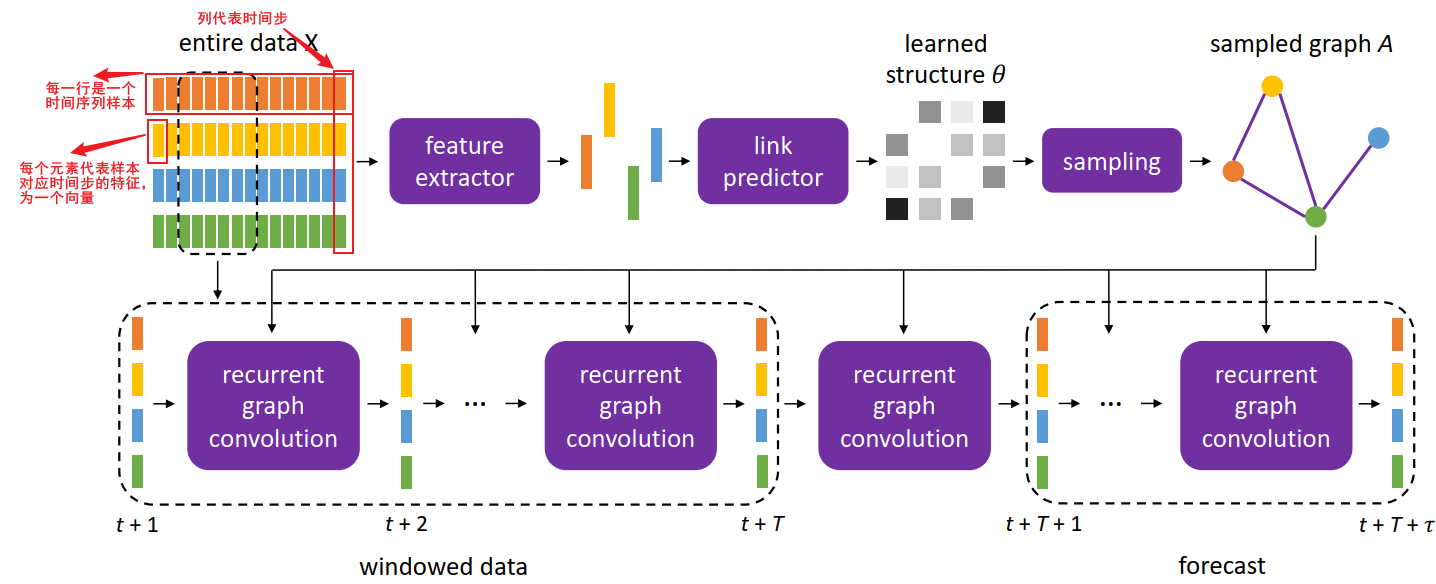
\includegraphics[width=.9\textwidth]{pics/gts.png}
	\caption{GTS Architecture}
	\label{fig:gts}
\end{figure}
GTS(Graph for time series)框架如Fig.\ref{fig:gts}所示。
看一眼损失函数:
$$
\sum_{t} \ell\left(f\left(A, w, X_{t+1: t+T}\right), X_{t+T+1: t+T+\tau}\right)
$$
很明显,在训练过程中,类似于用滑动窗口在时间序列样本的时间方向上滑动,再计算损失。具体的计算公式不用纠结。上文中提到了,要构建一个graph,那怎么构建呢?

对于n个训练样本,可以构建一个n个结点的graph,剩下的就是邻接矩阵了。论文中将邻接矩阵中每个元素(论文中构建的是有向图)的取值服从于一个伯努利分布$\theta$。$\theta$也是训练过程中学习得参数,因为邻接矩阵是从$\theta$中采样出来的,因此文中使用了Gumbel\cite{jang2017categorical}重参数化技术。模型的前向过程从Fig.\ref{fig:gts}可以体现。

\paragraph{总结}
从模型的输入可以看出,模型针对的数据主要是样本数不变的场景,如交通预测中,而且每个样本的序列长度是一致的。可以看作是针对一个固定结点集的graph,预测其结点特征。可以看作是一个回归任务,文中使用的也是均方误差作为损失。

}{}

\ifthenelse{\boolean{cv}}{
\clearpage
\section{CV}
\subsection{U-Net: Convolutional Networks for Biomedical Image Segmentation}
\begin{center}

  \begin{tabular}{rp{16cm}lp{20cm}}%{rl}

  % after \\: \hline or \cline{col1-col2} \cline{col3-col4} ...

  论文地址:& \href{https://arxiv.org/pdf/1505.04597.pdf}{https://arxiv.org/pdf/1505.04597.pdf} \\
  来源:& LNCS, 2015 \\
  作者:& Ronneberger, Olaf and Fischer, et al. \\

  %源码:& \href{xxx}{xxx} \\

%  slides:& \href{http://yunshengb.com/wp-content/uploads/2017/03/nips_2018_r2l_workshop_talk.pdf}{{\footnotesize Convolutional Set Matching for Graph Similarity}}\\

  关键词:& \textbf{Image Segmentation, Bimedical Image} \\

  写于:& \date{2021-04-19}

  \end{tabular}

\end{center}

该论文\cite{ronneberger2015u-net}提出的U-Net,是较早将卷积神经网络应用到图像语义分割的模型。U-Net是在FCN\cite{long2015fully}的基础上构建的。U-Net包含contracting path来提取图像特征/上下文、expanding path来进行精确的分割。

\paragraph{Motivation}
CNN通常用被用于分类,并且需要大量的数据。然而在医学图像处理任务中,不仅仅是对图像分类,还需要对图像进行逐像素的分割,而且通常无法获得大量的医学图像数据。在之前的一些方法中,将像素周围的局部区域划分为一个patch来预测一个像素的类别,这样获得的patch的数量远远大于图像的数量。但是这种方法有两个明显的缺点:1)速度慢,因为需要单独计算每个patch来预测像素类别,而且patch之间存在巨大的冗余;2)预测的准确率受所使用的patch的size的影响。还有一些方法使用不同层级的feature map来进行分割(如金字塔模型)。

鉴于已有方法的缺陷,U-Net在FCN\cite{long2015fully}的基础上进行修改和扩充,使得U-Net能够在数据量小的情况下得到更好的、高精度的分割效果。

\paragraph{U-Net}
U-Net结构如Fig.\ref{fig:unet}所示。
\begin{figure}[h]
	\centering
	\includegraphics[width=.8\textwidth]{pics/unet.png}
	\caption{U-Net architecture}
	\label{fig:unet}
\end{figure}
U-Net整体可以分为两部分,左边的压缩路径部分和右边的扩展路径部分。

在压缩路径上,输入的源图像经过卷积、max-pooling,尺寸逐渐变小,尺寸每为原来的二分之一,通道数则变为原来的两倍。在扩展路径上,feature map经过up-conv、卷积,尺寸逐渐增大,尺寸每变为原来的两倍,通道数变为原来的二分之一。除了左右两边的路径,U-Net还会将左边的压缩路径上的feature map裁剪一部分与右边的扩张路径同层级的feature map在通道上进行拼接,如Fig.\ref{fig:unet}中间灰色箭头所示。

到目前为止,U-Net都是比较简洁明了的,现在来更深入地挖掘一下。

\par{\textbf{Overlap-tile strategy}} 使用U-Net对源图像进行分割时,我们可以看到输出的分割结果比源图像要小,为了使得U-Net能够对任意大小的图像进行无缝的(seamless)分割,U-Net使用了Overlap-tile strategy,如Fig.\ref{fig:overlap-tile}所示。
\begin{figure}[h]
	\centering
	\includegraphics[width=.8\textwidth]{pics/Overlap-tile strategy.png}
	\caption{Overlap-tile strategy}
	\label{fig:overlap-tile}
\end{figure}
对于很大的图像,进行分割时可能需要将其进行划分成符合网络输入的块,原本在源图像内处于内部的区域可能成为了块的边界,在对块进行分割时,可能会产生缝隙/无法与相邻块的分割结果对齐。为了解决这个问题,也为了维持分割结果的size,U-Net使用了Overlap-tile strategy,以块的边界为轴进行镜像对称来对块进行padding(这一点不是很确定,论文中原文是:\textit{only use the valid part of each convolution})。

\par{\textbf{损失函数}}
为了让U-Net对边界有更好的分割效果、对与相邻的同类区域也有较好的分割效果,U-Net使用了带权重的交叉熵损失函数,该损失函数在每个像素处对$p_{l(\boldsymbol{x})}(\boldsymbol{x})$与1的偏差进行了惩罚:
$$
E = \sum_{\boldsymbol{x} \in \omega} w(\boldsymbol{x}) log(p_{l(\boldsymbol{x})}(\boldsymbol{x}))
$$
其中$\boldsymbol{x} \in \Omega, \Omega \subsxet \mathbb{Z}^2$,$\boldsymbol{x}$表示像素位置,$l: \Omega \rightarrow {1, ..., K}$表示每个像素的真实标签。$p_{l(\boldsymbol{x})}$是$softmax$函数,$w: \Omega \rightarrow \mathbb{R}$表示像素的权重。使用$w$有两个原因:1)类别不平衡;2)强调分割边界。$w$定义如下:
$$
w(\boldsymbol{x}) = w_c(\boldsymbol{x}) + w_0 \cdot exp(-\frac{(d_1(\boldsymbol{x}) + d_2(\boldsymbol{x}))^2}{2\sigma^2})
$$
其中$w_c: \Omega \rightarrow \mathbb{R}$用于解决类别不平衡的问题,$d_1: \Omega \rightarrow \mathbb{R}$表示$\boldsymbol{x}$到最近的细胞的距离(因为该论文是针对细胞分割任务的,在其他任务中,个人认为可以理解为到最近的分割目标距离),$d_2: \Omega \rightarrow \mathbb{R}$表示$\boldsymbol{x}$到第二近的细胞的距离。$w_0, \sigma$为超参数。

\par{\textbf{Data Augmentation}}
由于训练数据较少,作者对数据进行了平移、旋转等增强,最重要的是弹性变形增强。

\paragraph{总结}

\begin{itemize}

	\item U-Net是较早使用多尺度特征进行图像分割的算法
	\item U形结构对后续的图像分割模型有很大的启发
	\item 由于valid convolution,输入与输出的大小不一致

\end{itemize}


}{}

\ifthenelse{\boolean{nlp}}{
\clearpage
\section{NLP}
\subsection{Embedding Words in Non-Vector Space with Unsupervised Graph Learning}
\begin{center}
	\begin{tabular}{rl}
		% after \\: \hline or \cline{col1-col2} \cline{col3-col4} ...
		论文地址:& \href{https://arxiv.org/abs/2010.02598}{https://arxiv.org/abs/2010.02598} \\
		源码地址:& \href{https://github.com/yandex-research/graph-glove}{graph-glove} \\
		关键词:& \textbf{embedding, representation learning} \\
		写于:& \date{2020-10-08}
	\end{tabular}
\end{center}
传统的word embedding通常是将词嵌入到向量空间中,\cite{10.1145/219717.219748}指出words可以形成具有隐式层次结构的图,词向量的质量与选取什么样的向量空间有很大的关系。针对这个问题,该论文\cite{ryabinin2020embedding}提出了GraphGlove,将词嵌入到带权图(weighted graph)中。在word相似性及相关任务中,该论文提出的方法取得了比嵌入到向量空间中更好的效果。\\
\textbf{方法---GraphGlove}\hspace{6pt} 每个word视作带权图(weighted graph)中的一个结点,\textbf{词之间的距离使用图中结点之间的shortest path来表示(与欧氏空间中距离的定义不同)}。使用PRODIGE\cite{mazur2019vector}从数据中学习,可以得到一个带权图以及图中边的权重;再将学习得到的带权图用于GloVe\cite{pennington-etal-2014-glove}算法,学习得到在非欧空间中的词向量,关键之处是替换GloVe的损失函数中词之间距离为图中结点之间的最短距离。\\
该论文与其他embedding方法不同的之处:将word嵌入到非欧空间,学习到的带权图就是这个非欧空间。

\subsection{Enhancing Extractive Text Summarization with Topic-Aware Graph Neural Networks}
\begin{center}
	\begin{tabular}{rp{6cm}lp{10cm}}%{rl}
		% after \\: \hline or \cline{col1-col2} \cline{col3-col4} ...
		论文地址:& \href{https://arxiv.org/abs/2010.06253}{https://arxiv.org/abs/2010.06253} \\
		%源码地址:& \href{https://github.com/mocherson/Exp_GNN}{ExpGNN} \\
		关键词:& \textbf{Document Summarization, GAT, BERT} \\
		写于:& \date{2020-10-15}
	\end{tabular}
\end{center}
该论文\cite{cui2020enhancing}针对抽取式文本摘要问题提出了一个基于GNN的方法。现有的抽取式的文档摘要算法中,是通过从文档中抽取一个句子序列作为文档的摘要,但是通常没有考虑句子之间的关系,论文针对这个问题,提出了Topic-GraphSum模型。
\begin{figure}[h]
	\centering
	\includegraphics[width=.75\textwidth]{pics/Topic-GraphSum.PNG}
	\caption{Overview of Topic-GraphSum}
	\label{fig:topic_grpah_sum}
\end{figure}

如Fig.\ref{fig:topic_grpah_sum}所示,Topic-GraphSum模型主要分为三个部分,NTM(Neural Topic Model)用于从文档中抽取话题,Document Encoder用于生成每个句子的一个表征,再用前两部生成的topics和句子构造一个Heterogeneous Graph,使用GAT对该异构图进行学习,再将每个句子的表征输入到Sentecnce Classifer中,输出每个句子是否在Summarization中。
}{}

\ifthenelse{\boolean{recsys}}{
\clearpage
\section{Recommender System}
\subsection{Factorization Machines}
\begin{center}

  \begin{tabular}{rp{16cm}lp{20cm}}%{rl}

  % after \\: \hline or \cline{col1-col2} \cline{col3-col4} ...

  论文地址:& \href{https://ieeexplore.ieee.org/stamp/stamp.jsp?tp=\&arnumber=5694074}{https://ieeexplore.ieee.org/stamp/stamp.jsp?tp=\&arnumber=5694074} \\
  来源:& ICDM, 2010 \\
  作者:& Steffen Rendle \\

  源码:& \href{https://github.com/srendle/libfm}{libFM} \\

%  slides:& \href{http://yunshengb.com/wp-content/uploads/2017/03/nips_2018_r2l_workshop_talk.pdf}{{\footnotesize Convolutional Set Matching for Graph Similarity}}\\

  关键词:& \textbf{ sparse data, tensor factorization, support vector machine} \\

  写于:& \date{2021-08-10}

  \end{tabular}

\end{center}

该论文\cite{rendle2010factorization}提出了一种新的模型 --- Factorization Machines(FM),本质上是一个类似于SVM, LR的实值特征预测函数,但是FM能够应对及其稀疏的数据(如推荐场景)、包含了特征间的交互。一些关键点:
\begin{itemize}
	\item combines the advantages of Support Vector Machines (SVM) with factorization models
	\item FMs are a general predictor working with any real valued feature vector
	\item FMs model all interactions between variables using factorized parameters
\end{itemize}

 
\paragraph{问题定义}
$$
y : \mathbb{R}^n \longrightarrow T
$$
$T$是目标域,可以是实数,也可以是$\{+, -\}$,其中$\mathbb{R}^n$可能是及其稀疏的。

\paragraph{FM}
先上公式:
$$
\hat{y}(\boldsymbol{x}) = w_0 + \sum_{i=1}^n w_i x_i + \sum_{i=1}^n \sum_{j = i+1}^n <\boldsymbol{v_i}, \boldsymbol{v_j}> x_i x_j
$$
模型的输入就是$\boldsymbol{x} \in \mathbb{R}^n$,线性部分的参数$\boldsymbol{w} \in \mathbb{R}^n$,二阶特征交叉的权重是$\boldsymbol{V} \in \mathbb{R}^{n \times k}$。$\boldsymbol{v_i}$表示输入向量中第$i$个特征的向量表示。

如果写成这样:
$$
\hat{y}(\boldsymbol{x}) = w_0 + \sum_{i=1}^n w_i x_i + \sum_{i=1}^n \sum_{j = i+1}^n w_{ij} x_i x_j
$$
那么交叉特征的权重组成的矩阵$\boldsymbol{W} = [w]_{ij}$将是一个对称矩阵,而且$\boldsymbol{W} = \boldsymbol{V} \boldsymbol{V}^T$(正定矩阵可以通过Cholesky矩阵分解方法分解为一个元素非负下三角与其转置的乘,但\tbc{red}{怎么保证$\boldsymbol{W}$是正定的呢?})。那么为什么要写出一开始那个形式呢?

如果交叉特征的权重写成对称矩阵$\boldsymbol{W}$的形式,那么对于特征$i, j$来说,要学习到$w_{ij}$则需要足够的样本满足一定条件:$x_i != 0 \cap x_j != 0$,当$x_i = 0 \cup x_j = 0$则对更新$w_{ij}$没有帮助。

而把交叉特征的权重写成$<\boldsymbol{v_i}, \boldsymbol{v_j}>$的形式则不同了,由于每个特征都有一个隐向量$\boldsymbol{v_i}$,$\boldsymbol{v_i}$的更新可以通过$x_i, x_j$更新,也可以通过$x_i, x_k$来更新,当然,要更新$\boldsymbol{v_i}$,对特征$x_i$是有要求,有什么要求呢?

先来对FM的公式的交叉特征部分进行一个化简:

\begin{align}
	& \sum_{i=1}^{n} \sum_{j=i+1}^{n}\left\langle\mathbf{v}_{i}, \mathbf{v}_{j}\right\rangle x_{i} x_{j} \label{step0} \\
	=& \frac{1}{2} \sum_{i=1}^{n} \sum_{j=1}^{n}\left\langle\mathbf{v}_{i}, \mathbf{v}_{j}\right\rangle x_{i} x_{j}-\frac{1}{2} \sum_{i=1}^{n}\left\langle\mathbf{v}_{i}, \mathbf{v}_{i}\right\rangle x_{i} x_{i} \label{step1} \\
	=& \frac{1}{2}\left(\sum_{i=1}^{n} \sum_{j=1}^{n} \sum_{f=1}^{k} v_{i, f} v_{j, f} x_{i} x_{j}-\sum_{i=1}^{n} \sum_{f=1}^{k} v_{i, f} v_{i, f} x_{i} x_{i}\right) \label{step2} \\
	=& \frac{1}{2} \sum_{f=1}^{k}\left(\left(\sum_{i=1}^{n} v_{i, f} x_{i}\right)\left(\sum_{j=1}^{n} v_{j, f} x_{j}\right)-\sum_{i=1}^{n} v_{i, f}^{2} x_{i}^{2}\right) \label{step3} \\
	=& \frac{1}{2} \sum_{f=1}^{k}\left(\left(\sum_{i=1}^{n} v_{i, f} x_{i}\right)^{2}-\sum_{i=1}^{n} v_{i, f}^{2} x_{i}^{2}\right) \label{step4}
\end{align}
稍微解释一下:
\begin{itemize}
	\item 从 式子.\ref{step0} 到 式子.\ref{step1} 的变化,需要注意$j$的索引从$i+1$变成了$1$,相当于计算了$<\boldsymbol{v_i}, \boldsymbol{v_j}>$,$<\boldsymbol{v_i}, \boldsymbol{v_j}>$,即计算了两遍,但是对角线上的元素只算了一遍,所以还要减去对角线上的元素
	\item 从 式子.\ref{step1} 到 式子.\ref{step2} 的变化只是展开了$\boldsymbol{v_i}$而已
	\item 从 式子.\ref{step2} 到 式子.\ref{step4} 的变化则是把$f$那一层的求和提出来了,再进行了一些变化:
	$$
	\begin{aligned}
		& \sum_i^{n} \sum_j{n} v_{if} v_{jf} x_i x_j \\
		=& \sum_i^n v_{if} x_i \sum_j^n v_{jf} x_j \\
		=& A \cdot \sum_i^n v_{if} x_i \qquad (let\: A = \sum_j^n v_{jf} x_j) \\
		=& A \cdot B \qquad (let \:B = \sum_i^n v_{if} x_i) \\
		=& (\sum_i^n v_{if} x_i)^2
	\end{aligned}
	$$
\end{itemize}
这个变化可以看出,FM的时间复杂度是$O(kn)$,通过梯度下降更新参数时:
\begin{equation}\nonumber
	\frac{\partial}{\partial \theta} \hat{y}(\mathbf{x})= \begin{cases}1, & \text { if } \theta \text { is } w_{0} \\ x_{i}, & \text { if } \theta \text { is } w_{i} \\ x_{i} \sum_{j=1}^{n} v_{j, f} x_{j}-v_{i, f} x_{i}^{2}, & \text { if } \theta \text { is } v_{i, f}\end{cases}
\end{equation}
可以看到更新$v_{if}$时,需要$x_i$不等于0的样本。

文中还讨论了FM与SVM和基于分解的模型的联系与区别。当数据很稀疏时,难以准确的学习到SVM的参数、通过变化输入特征,FM可以与一些基于分解的模型等价。

%\begin{figure}[h]
%	\centering
%	\includegraphics[width=.8\textwidth]{}
%	\caption{}
%	\label{}
%\end{figure}

\paragraph{总结}

\begin{itemize}
	\item 将交叉特征的参数矩阵分解,得到每个特征的隐向量,用特征隐向量的内积作为交叉特征的权重
	\item \tbc{red}{怎么保证$\boldsymbol{W}$是正定的呢?}
	\item 分析了FM与SVM和基于分解的模型的联系

\end{itemize}



\subsection{Wide \& Deep Learning for Recommender Systems}
\begin{center}

  \begin{tabular}{rp{16cm}lp{20cm}}%{rl}

  % after \\: \hline or \cline{col1-col2} \cline{col3-col4} ...

  论文地址:& \href{https://arxiv.org/pdf/1606.07792v1.pdf}{https://arxiv.org/pdf/1606.07792v1.pdf} \\
  来源:& DLRS, 2016 \\
  作者:& Heng-Tze Cheng, Levent Koc, et al. \\

  源码:& \href{https://github.com/shenweichen/DeepCTR-Torch/blob/master/deepctr_torch/models/wdl.py}{Wide\&Deep} \\

%  slides:& \href{http://yunshengb.com/wp-content/uploads/2017/03/nips_2018_r2l_workshop_talk.pdf}{{\footnotesize Convolutional Set Matching for Graph Similarity}}\\

  关键词:& \textbf{Recommender systems} \\

  写于:& \date{2021-08-15}

  \end{tabular}

\end{center}

该论文\cite{cheng2016wide}提出了一个新的模型用于App推荐的模型 --- Wide\&Deep,该模型结合了Wide模型(LR模型)和Deep模型(Deep Neural Network)。

\paragraph{问题定义}
在推荐系统中有一个挑战 --- \textbf{Memorization \& Generalization}。Memorization:学习频繁共现的物品/特征在历史数据中的关系。Generalization:根据关系的传递性,探索新的特征组合,即使未在训练数据中出现或很少出现的特征组合也能给出合适的推荐。Memorization可以通过Wide模型来解决,Generalization可以通过Deep模型来解决。


\paragraph{Wide\&Deep}
\begin{figure}[h]
	\centering
	\includegraphics[width=.95\textwidth]{pics/wide&deep.png}
	\caption{Wide\&Deep}
	\label{fig:wdl}
\end{figure}

\subparagraph{Wide Component}
Wide模型一般是一个广义的线性模型,如LR或者包含特征交叉的线性模型。

\subparagraph{Deep Component}
Deep模型是一个基于神经网络的模型。在输入层,Deep模型将类别变量进行嵌入得到dense embedding(即Fig.\ref{fig:wdl}中的 Dense Embedding)。

\subparagraph{Joint of Wide and Deep}
Wide模型和Deep模型是联合训练的,Wide\&Deep模型的输出等于Wide和Deep模型的输出加权求和。论文中使用FTRL(Follow-the-regularized-leader,其在处理诸如逻辑回归之类的带非光滑正则化项,如L1范数的优化问题上性能非常出色)\cite{mcmahan2011follow-the-regularized-leader}来优化Wide\&Deep模型。

在论文中,作者将类被特征转化为ID,将连续值特征按照值的分位数转换到[0,1]。


\paragraph{总结}

\begin{itemize}
	\item Memorization与Generalization的结合
	\item Wide\&Deep用于Ranking
\end{itemize}



\subsection{Deep Neural Networks for YouTube Recommendations}
\begin{center}

  \begin{tabular}{rp{16cm}lp{20cm}}%{rl}

  % after \\: \hline or \cline{col1-col2} \cline{col3-col4} ...

  论文地址:& \href{https://dl.acm.org/doi/pdf/10.1145/2959100.2959190}{https://dl.acm.org/doi/pdf/10.1145/2959100.2959190} \\
  来源:& RecSys, 2016 \\
  作者:& Paul Covington, Jay Adams, Emre Sargin \\

  %源码:& \href{xxx}{xxx} \\

%  slides:& \href{http://yunshengb.com/wp-content/uploads/2017/03/nips_2018_r2l_workshop_talk.pdf}{{\footnotesize Convolutional Set Matching for Graph Similarity}}\\

  关键词:& \textbf{recommender system, deep learning, scalability} \\

  写于:& \date{2021-08-18}

  \end{tabular}

\end{center}

该论文\cite{covington2016deep}介绍了Youtube进行视频推荐的方法。Youtube进行视频推荐时分为两个阶段,各自由一个深度模型负责:deep candidate generation model、 deep ranking model。

\begin{figure}[h]
	\centering
	\includegraphics[width=.6\textwidth]{pics/recsys.png}
	\caption{推荐系统整体架构}
	\label{fig:recsys}
\end{figure}
\paragraph{问题定义}
在Youtube的视频推荐中主要有三大挑战:
\begin{itemize}
	\item Scale
	\item Fressness :每秒都有大量的视频上传到Youtube和大量用户产生观看记录,推荐的视频要能够反映最新上传的视频和用户最新的交互行为
	\item Noise :用户的历史行为是稀疏的且受到很多不可观测的因素的影响,一般难以得到用户的显示的对视频评价数据。需要在这样的数据上构建推荐算法
\end{itemize}
推荐系统的整体架构如Fig.\ref{fig:recsys}所示。


\paragraph{CANDIDATE GENERATION}
这一部分完成相关视频召回,召回阶段要保证高的Precision(尽量把相关的挑出来)。文中将召回作为一个多分类任务:
$$
P\left(w_{t}=i \mid U, C\right)=\frac{e^{v_{i} u}}{\sum_{j \in V} e^{v_{j} u}}
$$
$w_t$表示在时刻$t$看的视频的类别,每个视频$i$就是一个类别(没错,这是一个类别多达百万的多分类任务),$V, U, C$分别表示视频集、用户、上下文,$u \in \mathbb{R}^n, v_i \in \mathbb{R}^n$分别表示<用户,上下文>的向量、视频的向量。这一步模型的结构如Fig.\ref{fig:can_gen}所示,在最后一层输出的是\textit{user vector u},这个模型的目标是:\tbc{red}{学习一个函数,该函数以用户历史行为和上下文为输入,输出用户的embedding}

\begin{figure}[h]
	\centering
	\includegraphics[width=.8\textwidth]{pics/candidate generation.png}
	\caption{Deep candidate generation model architecture}
	\label{fig:can_gen}
\end{figure}
嗯?不是说好的多分类吗,怎么变成了用户embedding了?在Fig.\ref{fig:can_gen}的顶部,最后一层的$Relu$的输出分别给到了serving和training两部分。送往training的部分确实会根据用户embedding计算类别概率,但是在serving时,是召回top N个视频,这时候只需要把用户embedding作为query在视频集里找到top N个相似的视频即可。

\subparagraph{训练数据的生成}为每个用户生成相同数量的训练样本,避免过于活跃的用户对损失函数产生过大的影响。而且由于涉及到极多类别的多分类问题,因此涉及到softmax的计算,为了加快速度,采用了负采样。

\subparagraph{特殊的特征}每秒都有大量的视频上传到Youtube,推荐最新上传的视频给用户是很重要的。一个视频在Youtube上的热门程度是不平稳的,但是召回模型对一个视频的预测的概率(热门程度)是平稳的,为了矫正这个问题,增加了一个$example age$特征,在训练时,样本的$example age$特征取值为$t_{max} - t_N$,其中$t_{max}$表示训练样本中最大的视频上传时间,$t_N$是样本的上传时间;在serving时,该特征为0.

\paragraph{RANKING}
这一部分对召回的视频进行排序,排序的依据是视频的期望观看时长,排序时要尽量保证高的Recall。如Fig.\ref{fig:ranking}所示,Ranking模型通过$weighted\:logistic$(\tbc{red}{在weighted LR中,输出样本$i$的odds会变成原来的$w_i$倍,$w_i$为$i$的权重})进行训练。

Ranking阶段的weighted LR中将正样本的观看时长作为样本权重,负样本的权重为1。通过训练得到了weighted LR的参数,得到每个视频被点击的概率,由于权重是视频时长,则odds就是该视频期望播放时长。

\begin{figure}[h]
	\centering
	\includegraphics[width=.8\textwidth]{pics/ranking.png}
	\caption{Deep ranking network architecture}
	\label{fig:ranking}
\end{figure}

\subparagraph{特征表示}处理特征时忽略了时序,这样或许有助于模型的泛化。为一个视频打分时,该用户与这个视频(或相似视频)之前的交互数据最具参考价值。

\paragraph{总结}

\begin{itemize}
	\item 将召回阶段作为一个极多类别的分类任务
	\item 排序阶段预测每个视频的期望播放时长
	\item 特征工程功不可没
\end{itemize}



\subsection{Field-aware Factorization Machines for CTR Prediction}
\begin{center}

  \begin{tabular}{rp{16cm}lp{20cm}}%{rl}

  % after \\: \hline or \cline{col1-col2} \cline{col3-col4} ...

  论文地址:& \href{https://www.csie.ntu.edu.tw/~cjlin/papers/ffm.pdf}{https://www.csie.ntu.edu.tw/~cjlin/papers/ffm.pdf} \\
  来源:& RecSys, 2016 \\
  作者:& Yuchin Juan, Yong Zhuang, et al. \\

  源码:& \href{https://www.csie.ntu.edu.tw/~cjlin/libffm/}{libffm} \\

%  slides:& \href{http://yunshengb.com/wp-content/uploads/2017/03/nips_2018_r2l_workshop_talk.pdf}{{\footnotesize Convolutional Set Matching for Graph Similarity}}\\

  关键词:& \textbf{Machine learning, Click-through rate prediction, Computational advertising, Factorization machines} \\

  写于:& \date{2021-08-28}

  \end{tabular}

\end{center}

该论文\cite{juan2016field-aware}提出了FM模型的一个变种 --- FFM(Field-aware Factorization Machines)。FFM最初是应用的CTR预测任务上,模型与FM很类似。FFM也做了二阶特征交叉,交叉特征的权重的计算方式与FM略微不同。

\paragraph{问题定义}
解决CTR预测问题中特征稀疏、特征交叉的问题。

\paragraph{FFM}
FFM中将$n$个特征进行了分组,得到$f$个field,每个特征在每个field中都有一个$k$维的向量表示。对于交叉特征$x_{j_1}\cdot x_{j_2}$,其中$x_{j1}$属于field $f_1$,$x_{j_2}$同理,其权重计算方式为:$\boldsymbol{w}_{j_1, f_2} \cdot \boldsymbol{w}_{j_2, f_1}$,其中$\boldsymbol{w}_{j_1, f_2} \in \mathbb{R}^n$表示特征$x_{j_1}$在field $f_2$中的向量表示。

\begin{figure}[h]
	\centering
	\includegraphics[width=.8\textwidth]{pics/ffm-sg.png}
	\caption{Training FFM with SGD}
	\label{fig:ffm-sg}
\end{figure}
使用SGD训练FFM的过程如Fig.\ref{fig:ffm-sg}所示,其中引用的公式$(5), (6), (7), (8), (9), (10)$分别是:
$$
\begin{aligned}
	&\boldsymbol{g}_{j_{1}, f_{2}} \equiv \nabla_{\boldsymbol{w}_{j_{1}, f_{2}}} f(\boldsymbol{w})=\lambda \cdot \boldsymbol{w}_{j_{1}, f_{2}}+\kappa \cdot \boldsymbol{w}_{j_{2}, f_{1}} x_{j_{1}} x_{j_{2}}\\
	&\boldsymbol{g}_{j_{2}, f_{1}} \equiv \nabla_{\boldsymbol{w}_{j_{2}, f_{1}}} f(\boldsymbol{w})=\lambda \cdot \boldsymbol{w}_{j_{2}, f_{1}}+\kappa \cdot \boldsymbol{w}_{j_{1}, f_{2}} x_{j_{1}} x_{j_{2}}
\end{aligned}
$$

$$
\begin{aligned}
	&\left(G_{j_{1}, f_{2}}\right)_{d} \leftarrow\left(G_{j_{1}, f_{2}}\right)_{d}+\left(g_{j_{1}, f_{2}}\right)_{d}^{2}\\
	&\left(G_{j_{2}, f_{1}}\right)_{d} \leftarrow\left(G_{j_{2}, f_{1}}\right)_{d}+\left(g_{j_{2}, f_{1}}\right)_{d}^{2}
\end{aligned}
$$

$$
\begin{aligned}
	&\left(w_{j_{1}, f_{2}}\right)_{d} \leftarrow\left(w_{j_{1}, f_{2}}\right)_{d}-\frac{\eta}{\sqrt{\left(G_{j_{1}, f_{2}}\right)_{d}}}\left(g_{j_{1}, f_{2}}\right)_{d}\\
	&\left(w_{j_{2}, f_{1}}\right)_{d} \leftarrow\left(w_{j_{2}, f_{1}}\right)_{d}-\frac{\eta}{\sqrt{\left(G_{j_{2}, f_{1}}\right)_{d}}}\left(g_{j_{2}, f_{1}}\right)_{d}
\end{aligned}
$$
Fig.\ref{fig:ffm-sg}中的$(5)$计算的是损失函数(包含了l2正则)关于$\boldsymbol{w}_{j_1, f_2}$的梯度,$(6)$同理。$(7)$则计算的是$(5)$中梯度的各个维度的平方和,$G$初始化为1,避免计算完后$G$太小导致$G^{-\frac{1}{2}}$太大,$(8)$同理。$(9)$则是对$\boldsymbol{w}_{j_1, f_2}$逐维度更新,其中$\eta$自定义的学习率,这就是实际更新交叉特征参数的步骤,$(7)$中计算的$G$相当于对梯度向量归一化(\tbc{red}{个人觉得论文上公式是不是写错了,$(7),(8)$中应该是$G_{j_1, f_2}$而不是$(G_{j_1,f_2})_d$}。

\paragraph{为什么要field-aware?}
FM相当于FFM的一个特例,只有1个field。与FM相比,FFM将特征分成多个fields,每个特征在每个field中都有一个向量表示(\tbc{red}{从这个角度看有点像解耦表征})。当一个特征$x_{j_1}$与其他特征组合时,FM只有一个向量用于计算,而FFM中,会根据另一个特征所属的field使用不同的向量进行计算,相当于对模型表达能力的一个细化,增强模型的表达能力。当然,FFM的参数量增加了,而且不可以像FM那样化简,因此其时间复杂度为$O(\bar{n}^2k)$,但FFM中隐向量的维度要远小于FM的维度。

\paragraph{Assign field to feature}
既然每个特征都属于一个field,那怎么划分呢?对于类别特征,很显然,一般都属于同一个field。对于数值特征,可以对其进行离散化后作为类别特征处理。还有一种就是单一特征的样本(只有一个特征),例如特征是文本的情况下,每个文本基本都是不一样的,如果都划分到一个field则退化成了FM,如果每个文本都是一个field则是很不实际的,因为一般样本的数量是很大的,对于这个问题论文中并没有进行给出方法,个人认为:将文本处理成向量,可以是bag of words,一些统计量、embedding等。

\paragraph{总结}

\begin{itemize}
	\item 将特征划分到fields,增强模型的表达能力,一个特征与不同field的特征交叉时使用不同的向量表示
	\item 能够应对较稀疏的数据,当数据不是很稀疏时可能提升不是很明显
	\item 数值特征和单一特征划分field是个值得探讨的问题

\end{itemize}



\subsection{DeepFM: A Factorization-Machine based Neural Network for CTR Prediction}
\begin{center}

  \begin{tabular}{rp{16cm}lp{20cm}}%{rl}

  % after \\: \hline or \cline{col1-col2} \cline{col3-col4} ...

  论文地址:& \href{https://www.ijcai.org/Proceedings/2017/0239.pdf}{https://www.ijcai.org/Proceedings/2017/0239.pdf} \\
  来源:& IJCAI, 2017 \\
  作者:& Huifeng Guo, Ruiming Tang, et al. \\

  %源码:& \href{xxx}{xxx} \\

%  slides:& \href{http://yunshengb.com/wp-content/uploads/2017/03/nips_2018_r2l_workshop_talk.pdf}{{\footnotesize Convolutional Set Matching for Graph Similarity}}\\

  关键词:& \textbf{CTR, FMs, Wide\&Deep} \\

  写于:& \date{2021-08-31}

  \end{tabular}

\end{center}

该论文\cite{huifeng2017deepfm}提出了基于FM的深度模型 --- DeepFM,用于解决CTR问题。DeepFM与Wide\&Deep模型很像,但也有一些不同。DeepFM将Wide\&Deep中的LR替换为FM;不需要做特征工作;Wide和Deep部分的输入是共享的。

\paragraph{问题定义}
针对CTR问题,样本的特征可以分成多个field,$x = [x_{field_1}, x_{field_2}, ..., x_{field_m}]$,$x_{field_i}$是$field i$的向量表示,如one-hot编码。 

\paragraph{DeepFM}
DeepFM的整体结构如Fig.\ref{fig:deepfm}所示。DeepFM由两个部分组成:FM component和Deep component,这两部分共享输入。自底向上模型包含了Sparse Feature、Dense Embedding、FM Layer、Hidden Layer和Output Units。

对于Sparse Feature中的每一个特征,有一个权重与之相乘得到线性部分,也就是一阶特征;特征隐向量用于计算交叉特征之间的重要性,也就是二阶特征。特征隐向量也会作为Deep部分的输入。FM的输出与Deep的输出相加后经过Sigmoid函数后得到最终的输出。
$$
\hat{y} = sigmoid(y_{FM} + y_{DNN})
$$

\begin{figure}[h]
	\centering
	\includegraphics[width=.8\textwidth]{pics/deepfm.png}
	\caption{Wide \& deep architecture of DeepFM}
	\label{fig:deepfm}
\end{figure}

\subparagraph{FM Component}
\begin{figure}[h]
	\centering
	\includegraphics[width=.8\textwidth]{pics/deepfm-fm.png}
	\caption{ The architecture of FM}
	\label{fig:deepfm-fm}
\end{figure}
FM部分的结构如Fig.\ref{fig:deepfm-fm}所示,与常规的FM没有很大区别。\tbc{red}{有个问题,从Fig.\ref{fig:deepfm-fm}看,各个field的Dense Embedding进行内积作为特征的权重,这么说的话每个field一个隐向量,Dense Embedded就是这个隐向量?}

在FM部分,可以学习到一阶和二阶的特征。

\subparagraph{Deep Component}
\begin{figure}[h]
	\centering
	\includegraphics[width=.8\textwidth]{pics/deepfm-deep.png}
	\caption{The architecture of DNN}
	\label{fig:deepfm-deep}
\end{figure}
Deep部分的结构如Fig.\ref{fig:deepfm-deep}所示。由于大部分特征都是稀疏的,为了输入神经网络中,Dense Embedding将稀疏的特征转化成稠密的向量。Dense Embedding的结构如Fig.\ref{fig:deepfm-embedding}所示。

\begin{figure}[h]
	\centering
	\includegraphics[width=.8\textwidth]{pics/deepfm-embedding.png}
	\caption{The structure of the embedding layer}
	\label{fig:deepfm-embedding}
\end{figure}
Dense Embedding层将$x_{field}$向量编码成低维的稠密向量,其计算过程如Fig.\ref{fig:embedding}所示。$e_{i} = x_i \cdot \boldsymbol{V}$,其中$x_i \in \mathbb{R}^n$是$field i$的向量表示,$\boldsymbol{V} \in \mathbb{R}^{n \times k}$每行表示一个特征的隐向量,$n$表示$field i$的特征数。很显然,\textbf{Dense Embedding层将$\boldsymbol{V}$作为参数}。如果$x_{i}$是one-hot,则$e_i$表示第$i$个特征的隐向量,即\textbf{将不为零的那个特征的隐向量作为其Dense Embedding的输出}。最终Dense Embedding的输出为:$a^{(0)} = [e_1, e_2, ..., e_m]$,$a^{(0)}$作为Hidden Layer的输入,接下来就是常规操作啦。

在Deep部分,可以学习到高阶的交叉特征。

\begin{figure}[h]
	\centering
	\includegraphics[width=.8\textwidth]{pics/embedding.pdf}
	\caption{Dense Embedding层计算方式}
	\label{fig:embedding}	
\end{figure}


最终,FM部分和Deep部分是联合训练的,整个模型的参数包括$w_i, \boldsymbol{V}, (\boldsymbol{W}^{(l)}, b^{(l)})$。

\paragraph{总结}

\begin{itemize}

	\item 与现有的一些模型,如FNN,不需要预先训练FM部分的隐向量,DeepFM通过联合训练得到隐向量
	\item DeepFM的FM和Deep部分共享输入
		

\end{itemize}



\subsection{Product-based Neural Networks for User Response Prediction}
\begin{center}
	
	\begin{tabular}{rp{16cm}lp{20cm}}%{rl}
		
		% after \\: \hline or \cline{col1-col2} \cline{col3-col4} ...
		
		论文地址:& \href{https://arxiv.org/pdf/1611.00144.pdf}{https://arxiv.org/pdf/1611.00144.pdf} \\
		来源:& ICDM, 2016 \\
		作者:& Yanru Qu, Han Cai, et al. \\
		
		%源码:& \href{xxx}{xxx} \\
		
		%  slides:& \href{http://yunshengb.com/wp-content/uploads/2017/03/nips_2018_r2l_workshop_talk.pdf}{{\footnotesize Convolutional Set Matching for Graph Similarity}}\\
		
		关键词:& \textbf{CTR, Deep Learning} \\
		
		写于:& \date{2021-09-06}
		
	\end{tabular}
	
\end{center}

该论文\cite{qu2016product-based}提出了一种新的层 --- Product-based Neural Networks,用于捕捉输入特征中不同域之间的交互模式。

\paragraph{问题定义}
解决CTR问题。已有的一些研究\cite{menon2011response, anhphuong2015factorization}表明Product操作有助于探索(explore)不同特征域之间关系。

\paragraph{PNN}
PNN整体结构如Fig.\ref{fig:pnn}所示。与其他的深度模型类似,每个输入的样本由多个field组成。经过Embedding Layer再输入到论文所提出的Product Layer。理一下模型的计算过程:
\begin{itemize}
	\item 原始输入$\boldsymbol{x}$被表示成$N$个filed,每个filed在$\boldsymbol{x}$中是$\boldsymbol{x}[start_i: end_i]$
	\item $\boldsymbol{x}$输入到Embedding Layer,进行field-wise,$field_i$的embedding为:$\boldsymbol{f_i} =\boldsymbol{W_0^i}\boldsymbol{x}[start_i: end_i]$
	\item Embedding Layer的输出进入Product Layer,这一层主要输出两个向量$\boldsymbol{l}_z, \boldsymbol{l}_p$,分别是\textbf{线性操作部分和乘积操作部分}。其中$\boldsymbol{z} = \{\boldsymbol{f_1}, ..., \boldsymbol{f_N}\},\: \boldsymbol{p} = \{p_{ij}\} = g(\boldsymbol{f_i}, \boldsymbol{f_j})$,其中$g$就是论文中提出的\textbf{Product}操作,$g$可以是内积也可以是外积。$\boldsymbol{l}_z = \boldsymbol{W}_z \boldsymbol{z}^T,\: \boldsymbol{l}_p = \boldsymbol{W}_p \boldsymbol{p}^p$,其中$\boldsymbol{W}_z \in \mathbb{R}^{D_1 \times N \times M},\: \boldsymbol{W}_p \in \mathbb{R}^{D_1 \times N \times N}$分别是Product Layer的权重,$D_1$是Hidden Layer1的神经元个数
	\item Product Layer的输出加上偏置$\boldsymbol{b_1}$一起输入Hidden Layer1,最终Hidden Layer1的输出:$\boldsymbol{l_1} = relu(\boldsymbol{l}_z + \boldsymbol{l}_p + \boldsymbol{b_1})$
	\item 接下来就是常规操作了,经过全连接层得到最终的输出,经过$sigmoid$得到预测值,作为CTR估计值
\end{itemize}


\begin{figure}[h]
	\centering
 	\includegraphics[width=.6\textwidth]{pics/pnn.png}
	\caption{PNN Architecture}
	\label{fig:pnn}
\end{figure}


\paragraph{关于Product操作}
$g$既可以是内积也可以是外积。当$g$是外积时,$g(\boldsymbol{f_i}, \boldsymbol{f_j})$就成了一个矩阵,为了降低时间复杂度和空间复杂度,论文中使用了叠加(Superposition)操作:
$$
\boldsymbol{p}=\sum_{i=1}^{N} \sum_{j=1}^{N} \boldsymbol{f}_{i} \boldsymbol{f}_{j}^{T}=\boldsymbol{f}_{\Sigma}\left(\boldsymbol{f}_{\Sigma}\right)^{T}, \quad \boldsymbol{f}_{\Sigma}=\sum_{i=1}^{N} \boldsymbol{f}_{i}
$$
实际上就是把所有field的embedding先求和再计算外积,最终依然得到$\mathbb{R}^{N \times N}$的矩阵。


\paragraph{总结}

\begin{itemize}
	\item $\boldsymbol{l}_z, \boldsymbol{l}_p$分别作为对特征的线性部分和特征交叉部分(有点Wide\&Deep的味道了)
	\item 外积操作进行了Superposition,对不同特征的对应维度求和,类似于对所有field的特征进行池化,这要求\textbf{不同特征的对应维度有相似的含义},\tbc{red}{但是不同field的embedding是通过不同的权重得到的 --- 位于不同的向量空间中,不同特征的同一维不具有可比性}
	
\end{itemize}



\subsection{Personalized Video Recommendation Using Rich Contents from Videos}
\begin{center}
	
	\begin{tabular}{rp{16cm}lp{20cm}}%{rl}
		
		% after \\: \hline or \cline{col1-col2} \cline{col3-col4} ...
		
		论文地址:& \href{https://arxiv.org/pdf/1612.06935.pdf}{https://arxiv.org/pdf/1612.06935.pdf} \\
		来源:& TKDE, 2020 \\
		作者:& Xingzhong Du, Hongzhi Yin, et al. \\
		
		%源码:& \href{xxx}{xxx} \\
		
		%  slides:& \href{http://yunshengb.com/wp-content/uploads/2017/03/nips_2018_r2l_workshop_talk.pdf}{{\footnotesize Convolutional Set Matching for Graph Similarity}}\\
		
		关键词:& \textbf{Recommender model, personalization, video content analysis, rich content features, late fusion} \\
		
		写于:& \date{2021-09-06}
		
	\end{tabular}
	
\end{center}

在视频推荐中,现有的方法通常基于用户与视频的交互和单一的(视频)内容特征(如文本、音频等)进行推荐,当这个内容特征缺失时,推荐系统的性能将会受到很大的影响。该论文\cite{du2020personalized}针对这个问题,论文提出一种框架 --- collaborative embedding regression(CER)来解决这个问题。CER利用视频中丰富的内容特征,来弥补当某一种内容特征确实时带来的限制。另外,文中还提出了priority-based late fusion(PRI),用于获得集成多种内容特征带来的性能收益。

\paragraph{问题定义}
视频推荐中,很多方法只利用了视频的某一种特征,如文本、音频等,这会导致推荐系统在单一的特征缺失时效果不佳或者受制于冷启动问题。为了融合视频的多种特征以及能够在冷启动中也能取得良好的结果,论文提出了CER --- 将CF(Collaborative Filtering与任一视频特征结合,以及PRI --- 给出每种视频特征的优先级,来利用基于每种特征进行推荐时的结果。

\paragraph{xxx}

\paragraph{总结}

\begin{itemize}
	\item
	
\end{itemize}


}{}

\ifthenelse{\boolean{kt}}{
\clearpage
\section{Knowledge Tracing}
\subsection{Deep Knowledge Tracing}
\begin{center}
	
	\begin{tabular}{rp{16cm}lp{20cm}}%{rl}
		
		% after \\: \hline or \cline{col1-col2} \cline{col3-col4} ...
		
		论文地址:& \href{https://web.stanford.edu/~cpiech/bio/papers/deepKnowledgeTracing.pdf}{https://web.stanford.edu/~cpiech/bio/papers/deepKnowledgeTracing.pdf} \\
		来源:& NIPS, 2015 \\
		作者:& Chris Piech, et al. \\
		单位:& Stanford University, Khan Academy, Google \\
		源码:& \href{https://github.com/chrispiech/DeepKnowledgeTracing}{DeepKnowledgeTracing-lua}、\href{https://github.com/siyuanzhao/2016-EDM}{DeepKnowledgeTracing-py}\\
		
		%  slides:& \href{http://yunshengb.com/wp-content/uploads/2017/03/nips_2018_r2l_workshop_talk.pdf}{{\footnotesize Convolutional Set Matching for Graph Similarity}}\\
		
		关键词:& \textbf{Knowledge Tracing, RNN} \\
		
		写于:& \date{2021-09-22}
		
	\end{tabular}
	
\end{center}

该论文\cite{piech2015deep}使用RNN来对学生的知识水平进行追踪(Knowledge Tracing),提出了Deep Knowledge Tracing(DKT) --- 用RNN来捕捉学生与课程的交互序列,将学生的知识表示为可以学习的embedding。

\paragraph{问题定义}
\textbf{Knowledge Tracing(KT))}旨在对学生的只是进行建模,追踪学生的知识水平是如何随着与学生与课程交互而变化的。

能够准确地追踪学生的知识,有助于发现学生在学习过程中的薄弱点,更准确的引导学生学习 --- 有哪些知识点薄弱、哪些知识点已经掌握,更有针对性的查漏补缺。

KT的难点在于人类学习过程的复杂以及知识的表示的复杂:
\begin{itemize}
	\item 学习的过程是复杂的,涉及到多种对象
	\item 如何表示人的学习过程
	\item 人的知识水平如何体现
	\item 被学习的技能如何划分
	\item 学习材料如何学习内容相对应
	\item 人类在多种资料上学习:听说读写,甚至有动作,如何在在这些载体上追踪学生的知识
\end{itemize}


\textbf{形式化定义}:
在某个学习任务上,学生持续与相关的课程进行交互 --- 通常指做题,预测学生下一时刻回答某问题正确的概率。学生与课程的交互序列:$\boldsymbol{x_0}, \boldsymbol{x_1}, ..., \boldsymbol{x_t}$,通常$\boldsymbol{x_t} = \{q_t, a_t\}$表示$t$时学生做的题目以及学生的答案。

这篇论文的目的是\tbc{red}{基于学生以往的交互,预测学生对练习的作答情况}。

\paragraph{DKT}
DKT的模型比较简单,如Fig.\ref{fig:dkt}所示,有两个版本:一个基于普通的RNN、一个基于LSTM。

\begin{figure}[h]
	\centering
	\includegraphics[width=.35\textwidth]{pics/dkt.png}
	\caption{Deep Knowledge Tracing}
	\label{fig:dkt}
\end{figure}

模型的输入是学生的交互序列。DKT设定一共有$M$个练习,学生的每一次交互表示为:$\boldsymbol{x_t} = \{q_t, a_t\} \in \mathbb{R}^{2M}$。$q_t$表示学生回答的问题,$a_t$表示学生的作答,分别用one-hot表示。但是当$M$很大时,往往会带来过多的参数、难以训练等问题,因此,论文用一个dense vector表示一交互:$\boldsymbol{x_t} = \boldsymbol{n}_{q_t, q_t} \sim \mathcal{N}(0, \boldsymbol{I})$。

训练过程中使用交叉熵损失,评测指标是AUC。使用的数据集有:人工生成的模拟数据、Khan Academy Data、\href{https://sites.google.com/site/assistmentsdata/home/assistment-2009-2010-data}{Assistments benchmark dataset}。


\paragraph{总结}

\begin{itemize}
	\item 无需对练习进行标注(标注每个练习对应的知识点)
	\item 可以用于发现练习之间的关系 
	\item 第一个使用深度模型做Knowledge Tracing的
\end{itemize}



\subsection{Graph-based Knowledge Tracing: Modeling Student Proficiency Using Graph Neural Network}
\begin{center}
	
	\begin{tabular}{rp{16cm}lp{20cm}}%{rl}
		
		% after \\: \hline or \cline{col1-col2} \cline{col3-col4} ...
		
		论文地址:& \href{https://dl.acm.org/doi/pdf/10.1145/3350546.3352513}{https://dl.acm.org/doi/pdf/10.1145/3350546.3352513} \\
		来源:& WI, 2019 \\
		作者:& Hiromi Nakagawa, et al. \\
		单位:& The University of Tokyo$_{\times 3}$ \\
		源码:& \href{https://github.com/jhljx/GKT}{GKT} \\
		
		%  slides:& \href{http://yunshengb.com/wp-content/uploads/2017/03/nips_2018_r2l_workshop_talk.pdf}{{\footnotesize Convolutional Set Matching for Graph Similarity}}\\
		
		关键词:& \textbf{Knowledge Tracing, GNN} \\
		
		写于:& \date{2021-09-22}
		
	\end{tabular}
	
\end{center}

该论文\cite{nakagawa2019graph-based}将课程表达为一个Graph,将知识追踪问题转化为时间序列的结点分类问题,并提出了Graph-based Knowledge Tracing(GKT)。

\paragraph{问题定义}
从课程的组成结构来看,更像是一个有向图的结构,图中的结点是知识点,边表示知识点之间的依赖关系。 以往的Knowledge Tracing模型并没有考虑课程潜在的graph结构。 

GKT将一个课程(coursework)的知识分解为一定数量的知识概念,以知识概念作为结点,概念之间的依赖关系作为边构建graph。学生的知识水平是以其对课程中知识点的掌握程度/熟练程度来衡量的。一个学生与某个知识点进行交互,影响的不只是该知识点,还有依赖于该知识点的知识点和该知识点依赖的知识点。

但是在现实中,课程的图结构并不是显示存在的。\textbf{如何获得课程的图结构呢?}一种简单的思路是,依据数据中知识点的统计信息构建图;另一种思路是,通过一些基础的任务来学习出图的结构,这其中就涉及到GNN中的边特征学习。

形式化定义一下:
一门课程表示为:$G = (V, E),\:\: V=\{v_1, ..., v_N\},\:\: E \subseteq V\times V$。$V$表示课程所包含的$N$个知识点,$E$表示知识点之间的依赖关系。论文中假设学生对知识点的掌握是动态的:用$\boldsymbol{h}^t = \{\boldsymbol{h}^t_{i \in V}\}$表示学生在$t$时的知识状态。当学生与一个结点交互时,该结点及其一阶邻居的$\boldsymbol{h}$都会被更新。



\paragraph{GKT}
GKT的流程如Fig.\ref{fig:gkt}所示。GKT的关键有二:1)工作流程;2)如何得到隐式的课程graph。
\begin{figure}[h]
	\centering
	\includegraphics[width=.9\textwidth]{pics/gkt.png}
	\caption{GKT流程}
	\label{fig:gkt}
\end{figure}

\subparagraph{工作流程}结点的更新缘自学生的与课程的交互。流程分为三步走:
\begin{enumerate}
	\item Aggregates:根据$t$时的交互汇集相关结点的$\boldsymbol{h}^t_{i}$。交互表示为:$\boldsymbol{x}_t \in \{0, 1\}^{2N}$,表示的含义为交互的知识点和学生的答案
	\item Update:将汇集后的结点状态进行转换后输入到GRU中得到结点$t+1$时的$\boldsymbol{h}^{t+1}$
	\item Predict:基于$\boldsymbol{h}^{t+1}$预测学生对每个知识点进行回答时正确的概率
\end{enumerate}
工作流程比较常规,与结点预测任务的流程基本一样。

\subparagraph{隐式的图结构}因为课程的graph结构是静态的,因此如何得到隐式结构也就等于如何得到邻接矩阵$\boldsymbol{A}$。论文中给出了两种方法。
\par{Statistics-based Approach} 从数据的统计信息中得到邻接矩阵,论文中给出了三种构建的方法,不赘述。
\par{Learning-based Approach} 学习的方法重点也是在如何得到邻接矩阵,只不过矩阵中的值是在学习过程中得到的,也不赘述。

论文采用的数据集:\href{https://sites.google.com/site/assistmentsdata/home/assistment-2009-2010-data/skill-builder-data-2009-2010}{ASSISTments}和\href{https://pslcdatashop.web.cmu.edu/KDDCup/}{KDDCup-2010},指标是AUC。

\paragraph{总结}

\begin{itemize}
	\item 基于图结构、知识点随时间变化的状态表示学生的知识水平
	\item 支持多种方式得到隐式的图结构
	\item 如何得到知识点和回答的Embedding没有在文中解答
	\item 不同的学生学习同一门课程时使用的是相同的课程graph,但是如何针对每个学生给出初始的结点状态、训练样本是如何构造的没有详细描述
\end{itemize}



\subsection{Towards an Appropriate Query, Key, and Value Computation for Knowledge Tracing}
\begin{center}
	
	\begin{tabular}{rp{16cm}lp{20cm}}%{rl}
		
		% after \\: \hline or \cline{col1-col2} \cline{col3-col4} ...
		
		论文地址:& \href{https://arxiv.org/pdf/2002.07033.pdf}{https://arxiv.org/pdf/2002.07033.pdf} \\
		来源:& L@S, 2020 \\
		作者:& Youngduck Choi, et al. \\
		单位:& Riiid! AI Research, Yale University, University of Michigan, UC Berkeley \\
		源码:& \href{https://github.com/arshadshk/SAINT-pytorch}{SAINT} \\
		
		%  slides:& \href{http://yunshengb.com/wp-content/uploads/2017/03/nips_2018_r2l_workshop_talk.pdf}{{\footnotesize Convolutional Set Matching for Graph Similarity}}\\
		
		关键词:& \textbf{Knowledge Tracing, Student assessment, Transformer} \\
		
		写于:& \date{2021-09-22}
		
	\end{tabular}
	
\end{center}

该论文\cite{youngduck2020towards}针对当前Transformer和基于注意力的Knowledge Tracing模型的缺点,提出了基于Transformer的Knowledge Tracing模型 --- Separated Self-AttentIve Neural Knowledge Tracing(SAINT)。在SAINT中,练习和回答的embedding序列分别进入encoder和decoder部分。

\paragraph{问题定义}
\begin{figure}[h]
	\centering
	\includegraphics[width=.65\textwidth]{pics/saint-prev-methods.png}
	\caption{Architectures of Previous Methods}
	\label{fig:saint-prev}
\end{figure}
提出SAINT是为了解决现有的基于注意力的Knowledge Tracing的模型(如Fig.\ref{fig:saint-prev}所示)的两个局限:
\begin{itemize}
	\item 注意力层太浅,难以捕捉练习和回答之间复杂的关系
	\item 没有使用合适的方法构造注意力中的query, key, value
\end{itemize}

SAINT将练习和回答的embedding分别输入到SAINT的encoder和decoder部分(注意与Fig.\ref{fig:saint-prev}区别)。

形式化定义:

学生的行为序列:$\boldsymbol{I}_1, ..., \boldsymbol{I}_n$,其中$\boldsymbol{I}_i = \{E_i, R_i\}$,$E_i$表示第$i$个交互中的练习的信息,$R_i$表示学生此次练习的作答信息。SAINT的目标:$P(R_k = 1 | \boldsymbol{I}_1, ..., \boldsymbol{I}_{k-1}, E_k)$。

\paragraph{SAINT}
\begin{figure}[h]
	\centering
	\includegraphics[width=.38\textwidth]{pics/saint.png}
	\caption{Architecture of SAINT}
	\label{fig:saint}
\end{figure}
SAINT的模型结构如Fig.\ref{fig:saint}所示。$E_i, R_i$可以包含多种属性,如ID、类别、做题化的时间等,SAINT会先将原始的信息转换为embedding,则输入到SAINT是转换后的embedding序列。

SAINT的工作流程基本与Transformer一致。

论文中使用的数据集为\href{https://github.com/riiid/ednet}{EdNet}(关于英语教育,规模较大),使用的指标是AUC。

\paragraph{总结}

\begin{itemize}
	\item 将练习和回答分别作为encoder和decoder的输入,基于Transformer预测学生的知识水平
	%\item 
	
\end{itemize}



\subsection{Tracing Knowledge State with Individual Cognition and Acquisition Estimation}
\begin{center}
	
	\begin{tabular}{rp{16cm}lp{20cm}}%{rl}
		
		% after \\: \hline or \cline{col1-col2} \cline{col3-col4} ...
		
		论文地址:& \href{https://dl.acm.org/doi/pdf/10.1145/3404835.3462827}{https://dl.acm.org/doi/pdf/10.1145/3404835.3462827} \\
		来源:& SIGIR, 2021 \\
		作者:& Ting Long, et al. \\
		单位:& Shanghai Jiao Tong University$_{\times 5}$ \\
		源码:& \href{https://github.com/githubg0/iekt}{iekt} \\
		
		%  slides:& \href{http://yunshengb.com/wp-content/uploads/2017/03/nips_2018_r2l_workshop_talk.pdf}{{\footnotesize Convolutional Set Matching for Graph Similarity}}\\
		
		关键词:& \textbf{Knowledge Tracing, Student assess·ment, Transformer} \\
		
		写于:& \date{2021-09-23}
		
	\end{tabular}
	
\end{center}

该论文\cite{long2021tracing}提出了一种考虑学生认知水平和获取水平时的Knowledge Tracing方法 --- Individual Estimation Knowledge Tracing(IEKT)。

\paragraph{问题定义}
以往的Knowledge Tracing方法中,默认学生的认知水平(cognition level)是不变的,且不同的学生对同样的问题给出相同的作答后,学生的只是增长是一样的。然而实际情况:不同的学生由于不同的知识水平,完成相同的练习后知识的增长是不一样的。为什么以往的方法会有以上问题呢?1)没有显示地建模学生的认知水平/能力;2)没有显示地建模学生在不同地认知和知识水平下通过练习所能获得的知识。

形式化定义:
学生的练习记录:$\mathcal{X}_{t-1} = \{(q_1, r_1), ..., (q_{t-1}, r_{t-1})\}$,$(q_t, r_t)$表示学生在$t$时做的练习及学生的回答,且$r_t \in \{0, 1\}$。
\begin{table}[h]
	\centering
	\caption{符号说明}
	\label{tab:annotation}
	\begin{tabular}{ll}
		\hline Notations & Descriptions \\
		\hline$\mathcal{X}_{t-1}$ & Student's question-answering history. \\
		$q_{i}, c_{j}$ & The question and the concept. \\
		$Q, C$ & The set of questions and the set of concepts. \\
		$\mathbf{e}_{i}^{q}, \mathbf{e}_{j}^{c}$ & The embedding of question and concept. \\
		$\hat{r}_{t}, r_{t}$ & The predicted probability and the true label. \\
		$\mathbf{M}, \mathbf{m}_{t}$ & The cognition matrix and the cognition vector. \\
		$\mathbf{S}, \mathrm{s}_{t}$ & The acquisition matrix and the accquistion vector. \\
		$\mathbf{h}_{t}$ & The knowledge state. \\
		\hline
	\end{tabular}
\end{table}
论文中相关符号说明如Tab.\ref{tab:annotation}所示。其中,每个问题$q_i$可以与多个知识点相关,每个问题$q_i$和知识点$c_i$都有对应的embedding $\boldsymbol{e}_i^q, \boldsymbol{e}_i^c$(这两者的embedding是提前准备好的),每个学生在时刻$t$的知识状态为$\boldsymbol{h}_t$。

IEKT的目标:$P(r_t | q_t, \mathcal{X}_{t-1})$。

\paragraph{IEKT}
IEKT的模型是基于GRU的,可以分为两个阶段:read和write。read的任务是预测学生的回答$\hat{r}_t$,write的任务是更新学生的知识状态$\boldsymbol{h}_t$,模型结构如Fig.\ref{fig:iekt}(b)所示。
\begin{figure}[h]
	\centering
	\includegraphics[width=\textwidth]{pics/iekt.png}
	\caption{The frameworks and details of IEKT}
	\label{fig:iekt}
\end{figure}

整体来看,IEKT的工作流程和其他的RNN-based模型没有很大的差别,但是IEKT在read和write阶段各引入了一个模块。

\par{\textbf{read}}\ \ \ \ IEKT在这阶段引入了Cognition Estimation(CE)模块。该模块的输入是学生的知识状态$\boldsymbol{h}_t$(也就是GRU的hidden state)和问题的表征$\boldsymbol{v}_t$(不是$\boldsymbol{e}^q$,问题表征由问题embedding和知识embedding生成,具体参见论文)。CE的输出被用于预测$\hat{r}_t$。关键在于CE的内部操作。IEKT将认知水平划分为$k$个层次,每个层次用一个向量表示,$k$个层次形成一个Cognition Matrix $\boldsymbol{M}$。CE内部会基于学生的知识状态、问题embedding和知识点embedding得到学生$t$时的cognition level。cognition level对应的向量会与学生的知识状态、问题embedding和知识点embedding一起被送进分类器去预测$\hat{r}_t$。CE内部结构见Fig.\ref{fig:iekt}(c)。

\par{\textbf{write}}\ \ \ \ IEKT在此阶段引入了Knowledge acquisition sensitivity estimation(KASE)。KASE的目的是更新学生的知识状态。IEKT将学生的knowledge acquisition sensitivity划分为$b$个层次,每个层次对应一个向量,$b$个层次形成一个knowledge acquisition sensitivity matrix $\boldsymbol{S}$。KASE内部会根据(问题的表征,学生的知识状态、预测回答、真实的回答)来选择对应的知识获取水平,再将知识获取水平与问题表征、真实回答拼接后送入GRU,GRU输出的hidden state即是学生下一时刻的知识状态。由此可见,学生的知识状态是保存在GRU中的。

另外,在CE和KASE中是是通过输入获取$\boldsymbol{M}, \boldsymbol{S}$的行索引来获取相应的向量的,这样的操作是不可导的,论文中采用强化学习中的策略梯度来实现的。除了一些显而易见的参数外,还有一些参数是需要学习的:知识点和问题的embedding $\boldsymbol{e}^c, \boldsymbol{e}^q$以及$\boldsymbol{M}, \boldsymbol{S}$。

论文中使用的数据集:ASSIST09、ASSIST12、EdNet和Junyi,使用的指标是ACC和AUC。

\paragraph{总结}

\begin{itemize}
	\item 显示地建模了学生的认知水平和知识获取水平。学生在不同的知识状态和认知水平下的知识获取能力是不一样的
	\item 将学生的知识状态保存在GRU的hidden state中
	%\item 
	
\end{itemize}



\subsection{Federated Deep Knowledge Tracing}
\begin{center}
	
	\begin{tabular}{rp{16cm}lp{20cm}}%{rl}
		
		% after \\: \hline or \cline{col1-col2} \cline{col3-col4} ...
		
		论文地址:& \href{https://dl.acm.org/doi/pdf/10.1145/3437963.3441747}{https://dl.acm.org/doi/pdf/10.1145/3437963.3441747} \\
		来源:& WSDM, 2021 \\
		作者:& Jinze Wu, et al. \\
		单位:& USTC$_{\times 6}$, Anhui University, iFLYTEK Research \\
		源码:& \href{https://github.com/bigdata-ustc/federated-deep-knowledge-tracing}{FDKT} \\
		
		%  slides:& \href{http://yunshengb.com/wp-content/uploads/2017/03/nips_2018_r2l_workshop_talk.pdf}{{\footnotesize Convolutional Set Matching for Graph Similarity}}\\
		
		关键词:& \textbf{Know;edge Tracing, Federated Learning} \\
		
		写于:& \date{2021-09-24}
		
	\end{tabular}
	
\end{center}

该论文\cite{wu2021federated}使用联邦学习来进行Knowledge Tracing。对于以往的方法,论文指出了三个弊端:
\begin{itemize}
	\item Data scarcity:数据不足,学生的学习行为数据通常分散在各个平台以及在线下完成(如何同时使用多个平台的数据)
	\item Different data quality:数据质量不一,各平台/学校的教学安排是不一样的,学生在不同平台上学习并不能连续。例如,不同平台教授Python的过程是不一样的(如何辨别质量低的数据)
	\item Data incompara bility:数据的不一致性,在不同平台学习的学生,他们的知识状态不具有可比性(如何使学生的知识状态一致/对齐)
\end{itemize}
为了解决以上问题,论文提出了一种基于联邦学习的,以Server-client为结构的Knowledge Tracing模型 --- Federated Deep Knowledge Tracing(FDKT)。Client使用单个平台的数据学习,Server负责汇集和更新Clients的参数。


\paragraph{问题定义}
\par{\textbf{Federated Learning(FL)}} 是一种\textbf{保障数据安全}的机器学习方法,一般会有多个clients和一个server,每个client(相当于一个模型)的原始数据都存储在本地,并且不会交换或转移,clients在server的协调下协作解决机器学习问题。

形式化定义:一共有$S$个独立的学校,对于学校$s$,共有$N_s$名学生,$s$中的学生使用问题集是$Q$。一个学生的学习记录:$r = \{(q_1, g_1), ..., (q_l, g_l)\}$,$q_l$表示问题,$g_l \in \{0, 1\}$表示回答。所有学校的问题都是和$K$个知识点相关的。FDKT为每个学校设置一个DKT模型。

\paragraph{FDKT}
FDKT分为clients和server,FDKT学习的过程是一个迭代的过程,在每一次迭代中,每个client需要完成:1)利用所在学习的数据训练DKT模型;2)评估数据的质量。server需要完成:1)接手clients的信息,包括数据质量和模型参数;2)为每个client更新模型参数。


\begin{figure}[h]
	\centering
	\includegraphics[width=.5\textwidth]{pics/fdkt.png}
	\caption{Federated Deep Knowledge Tracing Framework}
	\label{fig:fdkt}
\end{figure}

FDKT使用的数据集:Math、ASSIST,使用的指标:ACC、AUC、RMSE。

\paragraph{总结}

\begin{itemize}
	\item 考虑了跨平台的数据隐私保护问题
	\item 以联邦学习的方式,融合多个平台的数据,为每个平台训练Knowledge Tracing模型
	
\end{itemize}



\subsection{Learning Process-consistent Knowledge Tracing}
\begin{center}
	
	\begin{tabular}{rp{16cm}lp{20cm}}%{rl}
		
		% after \\: \hline or \cline{col1-col2} \cline{col3-col4} ...
		
		论文地址:& \href{https://dl.acm.org/doi/pdf/10.1145/3447548.3467237}{https://dl.acm.org/doi/pdf/10.1145/3447548.3467237} \\
		来源:& KDD, 2021 \\
		作者:& Shuanghong Shen, et al. \\
		单位:& USTC$_{\times 6}$, iFLYTEK Research\\
		源码:& \href{https://github.com/bigdata-ustc/EduKTM}{EduKTM} \\
		
		%  slides:& \href{http://yunshengb.com/wp-content/uploads/2017/03/nips_2018_r2l_workshop_talk.pdf}{{\footnotesize Convolutional Set Matching for Graph Similarity}}\\
		
		关键词:& \textbf{Knowledge Tracing, learning process, learning gain, forgetting effect} \\
		
		写于:& \date{2021-09-24}
		
	\end{tabular}
	
\end{center}

该论文\cite{shen2021learning}通过建模学生的学习过程来进行KT(Knowledge Tracing)。在以往的KT模型中,以高准确率为目标,认为高准确率代表准确的表示了学生的知识状态,这使得知识状态更多地与回答正确的练习相联系。除此之外,大部分DKT模型没有考虑learning gain(做完练习后对知识掌握水平的差别)和forgetting effect(学生的知识掌握水平会随着时间降低)。对此,论文提出了 Learning Processconsistent Knowledge Tracing (LPKT)。

\paragraph{问题定义}
形式化定义:练习集合$E = \{e_1, ..., e_J\}$,知识点集合$K = \{k_1, ..., k_M\}$,练习与知识点关系矩阵$Q \in \mathbb{R}^{J \times M}$表示每个练习包含了哪些知识点。

学生的学习过程表示为:$x = \{(e_1, at_1, a_1), it_1, (e_2, at_2, a_2), it_2, ..., (e_t, at_t, a_t), it_t\}$,其中$(e_i, at_i, a_i)$表示一个learning cell,分别表示练习、练习用时、回答,$it_i$表示相邻learning cell的时间间隔。LKPT将练习、回答、回答用时、时间间隔都转化为embedding。

LPKT的目标是给定学习序列,监控学生的知识状态以及预测学生回答下一个问题正确的可能性。

\paragraph{LPKT}
LPKT显示地建模了learning gain和forgetting effect。
\par{\textbf{learning gain}}\ \ \ \ LPKT将$t$时地learning cell转化为embedding $\boldsymbol{l}_t$,基于$\boldsymbol{l}_{t-1}, \boldsymbol{l}_t$和$it_t$的embedding得到$t$时的learning gain $\boldsymbol{lg}_t$,再将$\boldsymbol{lg}_t$通过learning gate(是一个向量,主要考虑的是学生吸收知识的能力)得到学生真实的learning gain。

\par{\textbf{forgettign effect}}\ \ \ \ LKPT设计了forgetting gate(一个向量,用于表示遗忘程度)。学生的知识状态的更新基于learning gain、学生上一时刻的知识状态和forgetting gate。

最终的预测基于学生更新后的知识状态和$e_{t+1}$的embedding计算得到。

LPKT模型结构如Fig.\ref{fig:lpkt}所示。
\begin{figure}[h]
	\centering
	\includegraphics[width=\textwidth]{pics/lpkt.png}
	\caption{The architecture of the LPKT model}
	\label{fig:lpkt}
\end{figure}

论文使用的数据集:\href{https://sites.google.com/site/assistmentsdata/home/2012-13-school-data-withaffect}{ASSIST2012}、\href{https://sites.google.com/view/assistmentsdatamining/dataset}{ASSISTChall}、\href{http://ednet-leaderboard.s3-website-ap-northeast-1.amazonaws.com/}{EdNet-KT1},使用的指标有:RMSE、ACC、AUC、Pearson correlation。

\paragraph{总结}

\begin{itemize}
	\item LPKT考虑了learning gain和forgetting effect
	\item 将练习时间间隔加入到学习行为序列中
	\item 用矩阵表示学生的知识状态,每一行表示学生对一个知识点的掌握情况
	\item 只构建了练习与知识点之间的关系矩阵,\textbf{没有构建知识点之间的关系}
	
\end{itemize}



\subsection{Overview}
回顾Deep Knowledge Tracing。

\paragraph{Knowledge Tracing}动态地估计学生地知识状态,评估学生对各个知识点的掌握程度。知识状态通常表现为:$t$时刻,学生在练习上的作答情况。

在\textbf{学习某一课程}时,学生的学习行为序列:$\mathcal{X}_t = \{(q_1, r_1), ..., (q_t, r_t)\}$,其中$q_t$表示学生在$t$时回答的问题,$r_t$表示学生的回答。

现在,将Knowledge Tracing建模为:$P(r_t | q_t,\mathcal{X}_{t-1})$。

目前的Knowledge Tracing主要有以下几个特点:
\begin{itemize}
	\item $q_t$通畅为较为简单的问题、选择题,$r_t$为0或1
	\item 在学习过程中,通常为只学习一个\textit{skill}、\textit{course}的情况
	\item $q_i$通常作为知识点的载体,对应一个或多个知识点
	\item 没有考虑知识点之间的依赖关系
	\item 没有涉及到学生的知识状态的初始化问题,类似与“用户冷启动”
	\item 一个学生的知识状态,只与其历史行为相关
	\item 将学生在问题上的表现作为学生的知识状态(\tbc{red}{有无更好的表示学生知识水平的方法?})
	\item 大多数方法以预测准确率高为目标,模型的“注意力”主要集中在回答正确的问题上(\tbc{red}{从错误中学习}\cite{shen2021learning})
	\item 较少显示地考虑学生的学习/认知能力,练习对学生的状态地提升有多大(\cite{long2021tracing, shen2021learning})
	\item 较少地考虑到学生的知识随着时间而遗忘(\cite{shen2021learning})
\end{itemize}
}{}

\ifthenelse{\boolean{others}}{
\clearpage
\section{Others}
\subsection{Weakly-Supervised Disentanglement Without Compromises}
\begin{center}

  \begin{tabular}{rp{16cm}lp{20cm}}%{rl}

  % after \\: \hline or \cline{col1-col2} \cline{col3-col4} ...

  论文地址:& \href{https://arxiv.org/pdf/2002.02886.pdf}{https://arxiv.org/pdf/2002.02886.pdf} \\
  来源:& ICML, 2020\\
  作者:& Francesco Locatello, Ben Poole \\

  源码:& \href{https://github.com/google-research/google-research/tree/master/weak_disentangle}{weak\_disentangle} \\

%  slides:& \href{http://yunshengb.com/wp-content/uploads/2017/03/nips_2018_r2l_workshop_talk.pdf}{{\footnotesize Convolutional Set Matching for Graph Similarity}}\\

  关键词:& \textbf{generative model, disentangled representation, weakly-supervised generative model} \\

  写于:& \date{2021-01-22}

  \end{tabular}

\end{center}

该论文\cite{francesco2020weakly-supervised}是关于解耦表征学习的。论文提出的解耦表征学习方法从成对的图像中学习解耦表征,成对的图像之间存在一些区别,区别主要体现在隐因子的不同上。该方法只需要知道有几个隐因子变化了而不需要知道具体是哪几个。

\paragraph{解耦表征}目的是学习一个映射,该映射能够将数据映射到低维表示,表征是受潜在的因子控制的,每个潜在因子的变化能够使表征的一个或一些维度发生变化。这里所说的潜在因子与VAE中的隐变量很像。

我们可以假设任这世界上是有“终极”的,任何事物都是由一些因子/隐变量/终极特征所控制的。当我们用计算机来建模世界时,一些潜在的因子在控制表征。当进行表征学习时,我们用一个低维的向量来表示数据点,表征向量的某一(些)维发生变化对应着潜在因子的变化。有时我们学习的特征也学可以较好地应用于下游任务,但是它可能并不是解耦的。例如在AE中,我们可以学习到重建误差很小的表征,但是隐变量与表征之间的对应关系可能并不那么准确,如控制颜色的因子并没有与表征中的颜色部分相对应。从相关的角度来看,表征的不同维度(或者维度子集间)之间没有尽可能地无关。为什么会这样呢?因为在重建误差地指导下,习得地表征并不一定与隐变量之间有很准确的一一对应关系,虽然重建效果好但是可能难以被我们理解,表征地不同维度之间是相关的。

解耦表征的目的就是解决上述问题。解耦指的是表征的某个(些)维度与潜在因子之间解耦,即一个因子控制一个(些)表征的维度,一个(些)表征的维度受一个因子的控制。这样做有什么好处呢?首先,学习到的表征具有可解释性,对数据有更深层的理解;其次,可以控制表征的生成,知道表征与因子的对应关系可以实现可控的表征生成,相当于对表征空间有了更深入的了解;再者,对于下游任务,我们可以在解耦表征的基础上进行优化。

\paragraph{问题定义}其实,这篇论文呢我也没可能太懂,可能是里面的数学太多了。但是文章主要解决的问题是从成对儿的数据中学习到解耦表征。从论文的title可以看出,weakly-supervised。论文中的数据不需要知道有哪些因子,只需要知道有多少因子变化了即可,不需要对数据进行标注。

\paragraph{Disentangled Representation优点}
\begin{itemize}
	\item 解耦表征能够以压缩和可解释的结构包含原数据中的所有信息,并且表征与下游任务尽量无关
	\item 对下游的半监督或无监督学习任务有帮助,如迁移学习、少样本学习等
	\item 能够找出控制数据表征的重要factors

\end{itemize}






\subsection{Representation Learning via Invariant Causal Mechanism}
\begin{center}

  \begin{tabular}{rp{16cm}lp{20cm}}%{rl}

  % after \\: \hline or \cline{col1-col2} \cline{col3-col4} ...

  论文地址:& \href{https://arxiv.org/pdf/2010.07922.pdf}{https://arxiv.org/pdf/2010.07922.pdf} \\
  来源:& ICLR, 2021\\
  作者:& Jovana Mitrovic, Brian McWilliams, et al. \\

  %源码:& \href{xxx}{xxx} \\

%  slides:& \href{http://yunshengb.com/wp-content/uploads/2017/03/nips_2018_r2l_workshop_talk.pdf}{{\footnotesize Convolutional Set Matching for Graph Similarity}}\\

  关键词:& \textbf{Self-Supervised learning, Contrastive Learning, Causal} \\

  写于:& \date{2021-03-31}

  \end{tabular}

\end{center}

该论文\cite{mitrovic2021representation}从因果的视角下解释自监督学习,将数据生成过程看成由两个因子控制的过程。并且提出了RELIC(Representation Learning with Invariant Mechanisms),能够学习到尽量与下游任务无关的表征。

\paragraph{问题定义}
$X$表示未标记的数据,$\mathcal{Y} = \{Y_t\}_{t=1}^{T}$表示一系列未知的下游任务。目标就是使用$X$学习到有利于$\mathcal{Y}$的表征。

\paragraph{RELIC}
\begin{figure}[h]
	\centering
	\includegraphics[width=.3\textwidth]{pics/Causal.png}
	\caption{Data Generation in  Causal interpretation}
	\label{fig:causal}
\end{figure}
该论文主要针对的一个问题是:通过自监督学习到的表征尽量与下游任务无关。为了解决这个问题,作者将数据生成看作是有因果关系的,如Fig.\ref{fig:causal}所示。其中S,C分别表示Style和Content。并有三个前提假设:1)数据是由S,C生成的(有点变分推断\cite{kingma2014autoencoding}的味道);2)只有C与下游任务是相关的;3)C和S是不相关的。

在这里,S表示不同的数据增强方式。为了使数据的表则在不同的Style下是与下游任务是无关的,需要满足如下形式:
$$
p^{do(a_i)}(Y^R \:|\: f(X)) = p^{do(a_j)}(Y^R \:|\: f(X))\quad \forall a_i, a_j \in \mathcal{A}
$$
其中$p^{do(a_i)}$表示施加Style $a_i$后的数据分布,$\mathcal{A}$表示数据增强方式集合,即所有的styles。为了在不同的数据增强方式下对下游任务都是无关的,作者还提出了一个正则化项,最终的目标函数如下:
$$
\mathop{\mathbb{E}}\limits_{X} \mathop{\mathbb{E}}\limits_{a_{lk},a_{qt} \sim \mathcal{A} \times \mathcal{A}} \sum_{b \in\{a_{il,a_{qt}}\}} \mathcal{L}_b (Y^R, f(X))\quad s.t.\quad KL(p^{do(a_{lk})}(Y^R \:|\: f(X)), p^{do(a_{qt})}(Y^R \:|\: f(X))) \leq \rho
$$


\paragraph{总结}

\begin{itemize}

	\item 用因果解释自监督学习的过程,并且提出了使表征与下游任务无关的学习目标
	\item 看的不是很懂,还是太菜了

\end{itemize}



\subsection{UNSUPERVISED REPRESENTATION LEARNING FOR TIME SERIES WITH TEMPORAL NEIGHBORHOOD CODING}
\begin{center}

  \begin{tabular}{rp{16cm}lp{20cm}}%{rl}

  % after \\: \hline or \cline{col1-col2} \cline{col3-col4} ...

  论文地址:& \href{https://arxiv.org/pdf/2106.00750.pdf}{https://arxiv.org/pdf/2106.00750.pdf} \\
  来源:& ICLR, 2021 \\
  作者:& Sana Tonekaboni, Danny Eytan, Anna Goldenberg \\

  源码:& \href{https://github.com/sanatonek/TNC_representation_learning}{TNC} \\

%  slides:& \href{http://yunshengb.com/wp-content/uploads/2017/03/nips_2018_r2l_workshop_talk.pdf}{{\footnotesize Convolutional Set Matching for Graph Similarity}}\\

  关键词:& \textbf{time series, unsupervised representation learning} \\

  写于:& \date{2021-06-16}

  \end{tabular}

\end{center}

该论文\cite{tonekaboni2020unsupervised}针对的是(非平稳)时间序列数据的无监督表征问题,论文的Motivation来自Heathcare领域,患者的状态会在不同的临床状态之间转移。文中采用了对比学习的思想。

\paragraph{问题定义}
给定一个时间序列样本$X \in R^{D \times T}$,其中$T$该样本所跨越的时间长度,$D$表示样本在每一个时间步的特征维度。$X_{\left[t-\frac{\delta}{2}, t+\frac{\delta}{2}\right]}$表示$X$上的长度为$\delta$的时间窗口,因为该窗口以$t$为中心,我们表示为$W_t$。论文要解决的问题就是通过无监督学习得到$W_t$的表征。

\paragraph{TNC思路}
\begin{figure}[h]
	\centering
	\includegraphics[width=.9\textwidth]{pics/tnc.png}
	\caption{TNC Architecture}
	\label{fig:tnc}
\end{figure}
TNC框架如Fig.\ref{fig:tnc}所示。在问题定义中已经看到,论文是要学习一个时间窗口的表征,加上论文中使用了对比学习,因此很容易想到:对于一个$W_t$,需要采样正样本$W_l$与负样本$W_k$。既然如此,怎么采样就成了一个关键问题。

文中定义了\textbf{$W_t$的Temporal Neighborhood($N_t$)},以及Non Temporal Neighborhood($\bar{N_t}$)。显而易见,$W_l \in N_t, \: W_k \in \bar{N_t}$。既然如此,那么怎么定义Temporal Neighborhood呢?

说明白了,$N_t, \bar{N_t}$都是窗口的集合,那么只要给定窗口长度以及窗口中心就确定了一个窗口,通常窗口长度都是固定的,那么只需要确定窗口中心即可。论文中对$N_t$中的窗口中心$t^*$定义为:$t^{*} \sim \mathcal{N}(t, \eta \cdot \delta)$,其中$\eta$表示邻居的范围(\textbf{有点不解}),$\delta$表示窗口长度。作为时间序列的信号,通常有一个假设:信号局部是平稳的,即是光滑的。因此$N_t$中的窗口与$W_t$相似。$\eta$对于每个$t$都是不同的,$\eta$要尽量反映出信号保持静止(大致静止)的时间跨度,因此论文中使用了 Augmented Dickey-Fuller (ADF) 统计检验来为每个$W_t$计算$\eta$。

$\bar{N_t}$的采样,则是从与$t$有一定距离(从代码中可以看出这个距离是和$\eta$有关的)的范围内采样得到的。论文中并没有直接将$\bar{N_t}$中的样本当作负样本。原因是sample bias:从数据分布中随机采样的负样本有可能与参考样本是相似的。论文中将$ W_k \in \bar{N_t}$视作unlabeld 样本。从实践的角度来看:用一个参数$w$表示unlabeled 样本属于正样本的概率,因此一个unlabeled样本表示$w$个正样本与$1-w$个负样本的结合,在计算损失的时候,unlabeled 样本会分别作为正负样本与参考样本计算损失,再分别乘以$w, 1-w$作为这个unlabeled样本的损失。

$$
\mathcal{L}=-\mathbb{E}_{W_{t} \sim X}\left[\mathbb{E}_{W_{l} \sim N_{t}}[\log \underbrace{\mathcal{D}\left(Z_{t}, Z_{l}\right)}_{\mathcal{D}\left(\operatorname{Enc}\left(W_{t}\right), \operatorname{Enc}\left(W_{l}\right)\right)}]+\mathbb{E}_{W_{k} \sim \bar{N}_{t}}[\left(1-w_{t}\right) \times \log \underbrace{\left(1-\mathcal{D}\left(Z_{t}, Z_{k}\right)\right)}_{\mathcal{D}\left(\operatorname{Enc}\left(W_{t}\right), \operatorname{Enc}\left(W_{k}\right)\right)}+w_{t} \times \log \mathcal{D}\left(Z_{t}, Z_{k}\right)]\right]
$$

\textbf{流程}:获取一个参考样本$W_t$,在获取一个正样本$W_l$以及一个unlabeled样本$W_k$,分别传入一个编码器(通常是序列模型,可以是RNN,因为每个样本就是一个时间序列样本)中,分别得到表征$Z_t, Z_l, Z_k$。用一个判别器(其实就是一个分类器)分别计算$(Z_t, Z_l), \:(Z_t, Z_l)$一个分数(该样本对相似的度量),再计算对比损失,特别要注意$(Z_t, Z_l)$的损失哦!

\paragraph{总结}

\begin{itemize}

	\item 文中对unlabeled的想法很有趣
	\item 文中的实验通过聚类以及trajactory来发现序列随时间的变化,这也是我之前考虑过的一个问题
	\item 不知道用在图数据集上怎么样,挖掘图数据的变化,可以是graph-level的或者是node-level的

\end{itemize}


}{}
%\clearpagev
% \bibliographystyle{plain}
% \bibliography{bibfile}


% 打印参考文献
\printbibliography
\bibliographystyle{plain}
\bibliography{references}

\end{document}